% =============================================================================
% Sección 1.1: Objetivo del proyecto
% Generado por latex-writer | Fecha: 2026-03-25
% =============================================================================

\subsection{Objetivo del proyecto}
\label{subsec:objetivo-proyecto}

La presente memoria técnica tiene como objetivo el diseño y dimensionamiento de una instalación completa de vapor industrial destinada al suministro de energía térmica a una parcela industrial. El proyecto abarca tanto la red de distribución de vapor como la red de retorno de condensados, garantizando un funcionamiento eficiente y seguro conforme a la normativa vigente.

La instalación se ubica en la parcela A3 del polígono industrial de Salamanca, España, con referencia catastral 5183601TL9358S0001KH. La altitud de 700~m sobre el nivel del mar determina una presión atmosférica local de 0,932~bar, condición que ha sido considerada en todos los cálculos termodinámicos desarrollados.

El sistema está diseñado para operar con vapor sobrecalentado a una temperatura de 220~°C, generado mediante una caldera Viessmann VITOMAX 100-HS (modelo M33A) que opera a una presión de 10~bar(a). El caudal de diseño de la instalación es de 5400~kg/h, incluyendo un factor de seguridad del 15\% para compensar posibles fugas y pérdidas en el sistema.

La instalación suministra vapor a cuatro consumidores industriales con diferentes requerimientos de caudal y presión, tal como se detalla en la \tabref{tab:consumidores-proyecto}.

\begin{table}[H]
	\centering
	\caption{Consumidores de la instalación y sus requerimientos operativos}
	\label{tab:consumidores-proyecto}
	\begin{tabular}{ccc}
		\toprule
		\textbf{Consumidor} & \textbf{Caudal [kg/h]} & \textbf{Presión [bar(g)]} \\
		\midrule
		C1                  & 679                    & 4                         \\
		C2                  & 1359                   & 7                         \\
		C3                  & 340                    & 7                         \\
		C4                  & 2038                   & 7                         \\
		\bottomrule
	\end{tabular}
\end{table}

El alcance del presente proyecto comprende los siguientes aspectos técnicos:

\begin{enumerate}[label=\arabic*., leftmargin=2em]
	\item Dimensionamiento de la red de distribución de vapor, incluyendo el cálculo de diámetros, pérdidas de carga y velocidades en cada tramo.
	\item Dimensionamiento de la red de retorno de condensados, considerando la recuperación eficiente del condensado generado en los puntos de consumo.
	\item Selección y verificación de la caldera comercial adecuada para satisfacer la demanda térmica del sistema.
	\item Cálculo del aislamiento térmico de las tuberías en cumplimiento con el Reglamento de Instalaciones Térmicas en los Edificios (RITE).
	\item Gestión y aprovechamiento del vapor flash generado en los procesos de expansión del condensado.
	\item Diseño diferenciado de tramos aéreos y soterrados según las condiciones de instalación.
\end{enumerate}

Cabe destacar que el presente proyecto corresponde a una instalación existente, por lo que no se contemplan ampliaciones futuras. Todos los cálculos y dimensionamientos se han realizado considerando exclusivamente las condiciones de operación actuales y los consumidores definidos en la \tabref{tab:consumidores-proyecto}.

% =============================================================================
% Sección 1.2: Descripción de la planta y ubicación
% Generado por latex-writer | Fecha: 2026-03-25
% =============================================================================

\subsection{Descripción de la planta y ubicación}
\label{subsec:descripcion-planta-ubicacion}

La instalación de vapor objeto del presente proyecto se ubica en la parcela A3 del polígono industrial de Salamanca, España. La referencia catastral del emplazamiento es 5183601TL9358S0001KH. La altitud del terreno, situada a 700~m sobre el nivel del mar, condiciona las propiedades termodinámicas del vapor al reducir la presión atmosférica local a 0,932~bar, valor que ha sido considerado en todos los cálculos de dimensionamiento. La temperatura ambiente de diseño adoptada es de 15~°C.

Los parámetros de emplazamiento se resumen en la \tabref{tab:datos-ubicacion}.

\begin{table}[H]
	\centering
	\caption{Datos de ubicación y condiciones ambientales de diseño}
	\label{tab:datos-ubicacion}
	\begin{tabular}{lc}
		\toprule
		\textbf{Parámetro}             & \textbf{Valor}       \\
		\midrule
		Ciudad                         & Salamanca, España    \\
		Parcela                        & A3                   \\
		Referencia catastral           & 5183601TL9358S0001KH \\
		Altitud                        & 700~m s.n.m.         \\
		Presión atmosférica local      & 0,932~bar            \\
		Temperatura ambiente de diseño & 15~°C                \\
		\bottomrule
	\end{tabular}
\end{table}

La red de distribución de vapor está configurada mediante una topología ramificada que parte del punto de generación (caldera Viessmann VITOMAX 100-HS) y se bifurca progresivamente para alimentar a los cuatro consumidores industriales. La estructura de la red se articula en torno a tres nodos principales:

\begin{itemize}[leftmargin=2em]
	\item \textbf{Punto P:} Nodo de bifurcación principal situado a la salida de la caldera. Desde este punto se derivan dos ramales: uno hacia el consumidor C1 (tramo soterrado) y otro hacia el nodo secundario S (tramo aéreo).
	\item \textbf{Punto S:} Nodo secundario que distribuye el vapor hacia el consumidor C2 y hacia el nodo terciario T.
	\item \textbf{Punto T:} Nodo terciario desde el cual se alimentan los consumidores C3 y C4.
\end{itemize}

\begin{table}[H]
	\centering
	\caption{Tramos de la red de distribución de vapor}
	\label{tab:tramos-red-vapor}
	\begin{tabular}{lccc}
		\toprule
		\textbf{Tramo} & \textbf{Longitud [m]} & \textbf{Tipo} & \textbf{Diámetro} \\
		\midrule
		Caldera-P      & 12,74                 & Aéreo         & DN~150            \\
		P-C$_1$        & 88,19                 & Soterrado     & DN~80             \\
		P-S            & 106,00                & Aéreo         & DN~125            \\
		S-C$_2$        & 25,00                 & Aéreo         & DN~80             \\
		S-T            & 60,00                 & Aéreo         & DN~100            \\
		T-C$_3$        & 15,00                 & Aéreo         & DN~50             \\
		T-C$_4$        & 45,00                 & Aéreo         & DN~100            \\
		\midrule
		\textbf{Total} & \textbf{351,93}       & ---           & ---               \\
		\bottomrule
	\end{tabular}
\end{table}

La distribución de la parcela y la ubicación de los puntos de consumo se muestran en la \figref{fig:plano-parcela}.

\begin{figure}[H]
	\centering
	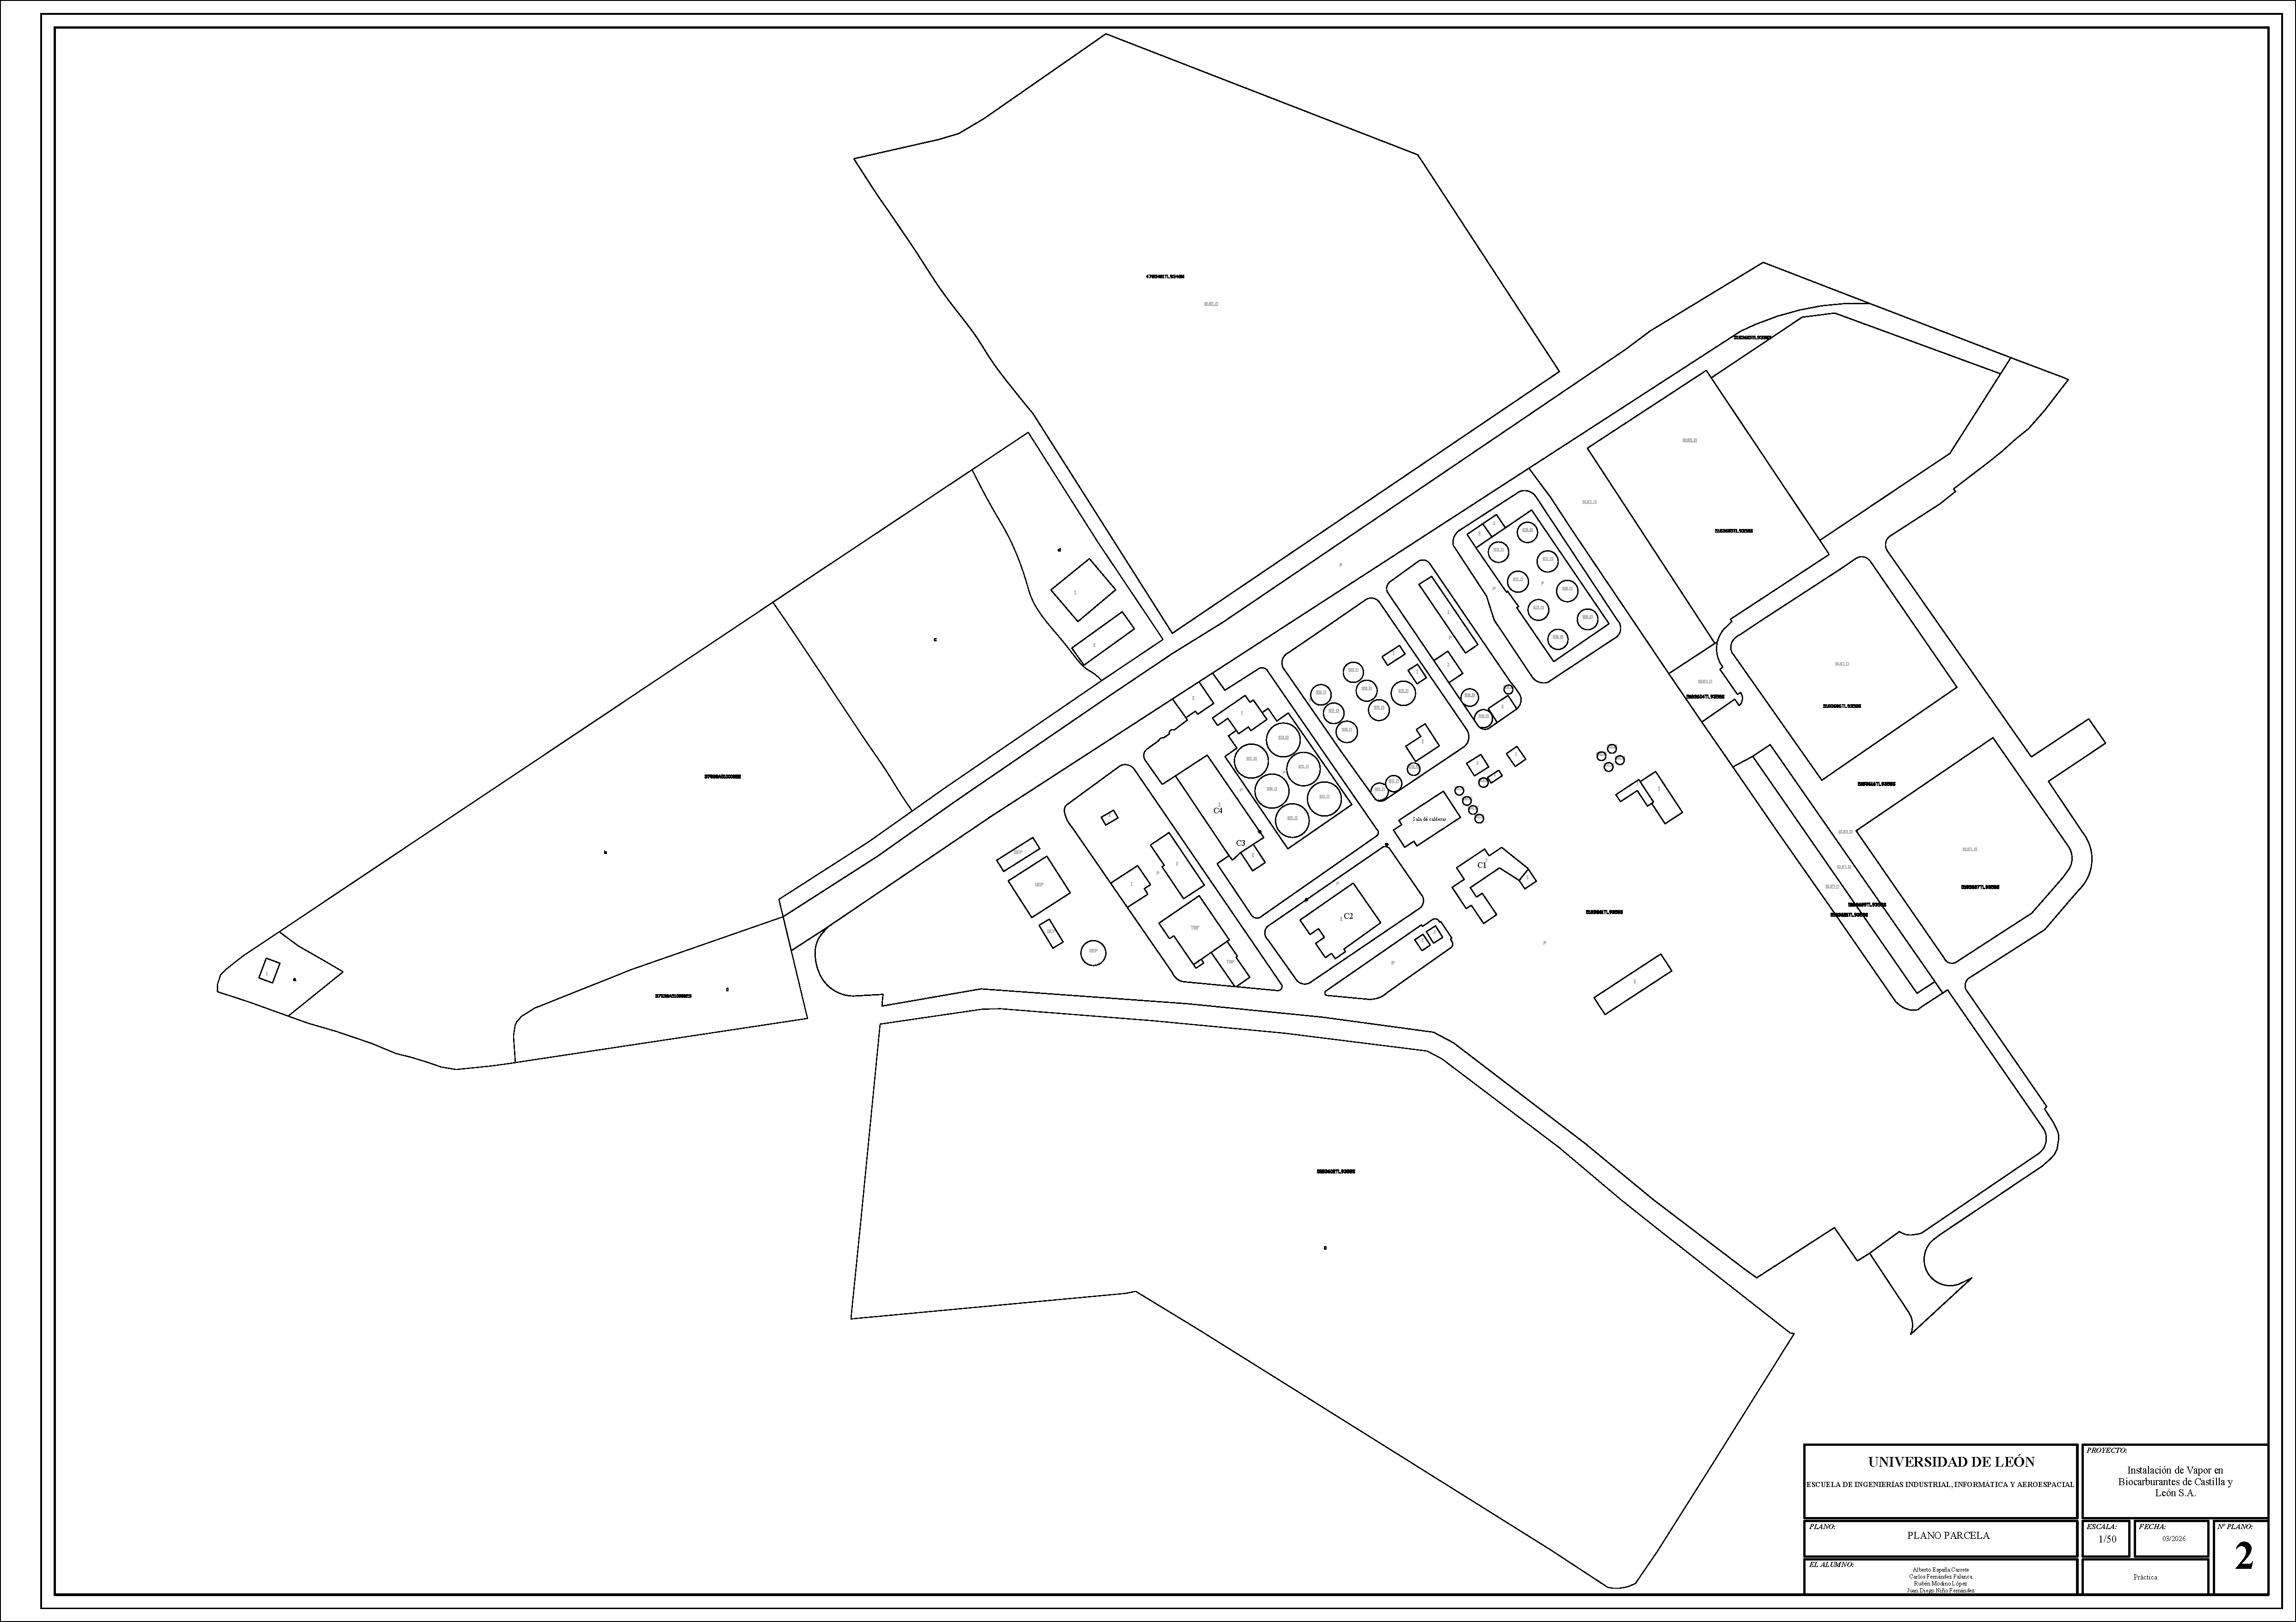
\includegraphics[width=0.85\textwidth]{Figuras/planos/plano_vapor-Parcela.pdf}
	\caption{Plano de la parcela A3 con distribución de la red de vapor}
	\label{fig:plano-parcela}
\end{figure}

Respecto al tipo de instalación, cabe distinguir entre tramos aéreos y soterrados. Los tramos aéreos, que constituyen seis de los siete tramos de la red, discurren a una altura comprendida entre 5 y 6~m sobre el nivel del suelo, soportados mediante estructuras metálicas y con accesibilidad directa para labores de mantenimiento. El único tramo soterrado corresponde a la conexión P-C$_1$, cuyo eje de tubería se sitúa a una profundidad de 1,09~m bajo la rasante del terreno. Este tramo soterrado requiere consideraciones especiales en cuanto al aislamiento térmico y la protección mecánica de la tubería, aspectos que serán desarrollados en las secciones correspondientes de la presente memoria.

% =============================================================================
% Sección 1.3: Puntos de consumo y requerimientos iniciales
% Generado por latex-writer | Fecha: 2026-03-25
% =============================================================================

\subsection{Puntos de consumo y requerimientos iniciales}
\label{subsec:puntos-consumo-requerimientos}

La instalación de vapor abastece a cuatro consumidores industriales (C1, C2, C3 y C4) con diferentes requerimientos de caudal y presión de operación. La caracterización precisa de estos puntos de consumo constituye el punto de partida para el dimensionamiento de la red de distribución, ya que determina tanto los caudales circulantes por cada tramo como las pérdidas de carga admisibles en el sistema.

Los datos de partida correspondientes a cada consumidor se presentan en la \tabref{tab:consumidores-requerimientos}, donde se indica el caudal demandado, la presión mínima requerida en el punto de consumo, la presión disponible tras considerar las pérdidas de carga en la red, y la distancia desde la caldera hasta cada punto de suministro.

\begin{table}[H]
	\centering
	\caption{Requerimientos de los puntos de consumo}
	\label{tab:consumidores-requerimientos}
	\begin{tabular}{ccccc}
		\toprule
		\textbf{Consumidor} & \textbf{Caudal [kg/h]} & \textbf{Presión requerida [bar(g)]} & \textbf{Presión disponible [bar(g)]} & \textbf{Distancia [m]} \\
		\midrule
		C1                  & 679                    & 4                                   & 8,818                                & 100,93                 \\
		C2                  & 1359                   & 7                                   & 8,830                                & 143,74                 \\
		C3                  & 340                    & 7                                   & 8,710                                & 193,74                 \\
		C4                  & 2038                   & 7                                   & 8,690                                & 223,74                 \\
		\bottomrule
	\end{tabular}
\end{table}

Del análisis de los datos presentados se desprende que el consumidor C4 representa el mayor demandante de vapor, con un caudal de 2038~kg/h que supone aproximadamente el 46\% del consumo total de la instalación. Por el contrario, el consumidor C3 presenta el menor requerimiento con tan solo 340~kg/h. Esta distribución heterogénea de caudales condiciona directamente el dimensionamiento de los diferentes tramos de la red.

\subsubsection{Cálculo del caudal total de diseño}

El caudal total de diseño de la instalación se determina a partir de la suma de los caudales individuales de cada consumidor, aplicando un factor de seguridad $K$ que contempla las pérdidas por fugas inherentes a cualquier red de distribución de vapor. El cálculo se realiza mediante la siguiente expresión:

\begin{equation}
	Q_{\text{total}} = K \cdot \sum_{i=1}^{4} C_i = 1{,}15 \cdot (679 + 1359 + 340 + 2038) = 1{,}15 \cdot 4416 = 5078{,}4 \ \text{kg/h}
	\label{eq:caudal-total-diseno}
\end{equation}

El factor de seguridad adoptado, $K = 1{,}15$, corresponde a un incremento del 15\% sobre el caudal nominal calculado. Este margen adicional compensa las inevitables fugas de vapor que se producen en juntas, válvulas, purgadores y demás elementos de la instalación, asegurando que la capacidad de generación sea suficiente para satisfacer la demanda real del sistema en condiciones de operación continua.

El caudal de diseño calculado de 5078,4~kg/h se ajusta al caudal comercial de la caldera seleccionada. La \tabref{tab:resumen-caudales} presenta un resumen de los valores característicos del dimensionamiento.

\begin{table}[H]
	\centering
	\caption{Resumen del cálculo de caudales de diseño}
	\label{tab:resumen-caudales}
	\begin{tabular}{lcc}
		\toprule
		\textbf{Parámetro}                        & \textbf{Valor} & \textbf{Unidad} \\
		\midrule
		Suma de caudales de consumidores          & 4416           & kg/h            \\
		Factor de seguridad ($K$)                 & 1,15           & ---             \\
		Caudal de diseño calculado                & 5078,4         & kg/h            \\
		Caudal comercial (caldera Vitomax 100-HS) & 5400           & kg/h            \\
		\bottomrule
	\end{tabular}
\end{table}

\subsubsection{Condiciones del vapor de suministro}

El vapor generado por la caldera Viessmann VITOMAX 100-HS corresponde a vapor sobrecalentado, condición que se mantiene a lo largo de la red de distribución. Las propiedades termodinámicas del vapor a la salida de la caldera se recogen en la \tabref{tab:condiciones-vapor}.

\begin{table}[H]
	\centering
	\caption{Propiedades del vapor a la salida de la caldera}
	\label{tab:condiciones-vapor}
	\begin{tabular}{lcc}
		\toprule
		\textbf{Propiedad}  & \textbf{Valor} & \textbf{Unidad} \\
		\midrule
		Tipo de vapor       & Sobrecalentado & ---             \\
		Temperatura         & 220            & °C              \\
		Presión de caldera  & 9,068          & bar(g)          \\
		Entalpía específica & 2874           & kJ/kg           \\
		\bottomrule
	\end{tabular}
\end{table}

\subsubsection{Consideraciones especiales para el consumidor C1}

El análisis de los requerimientos de presión revela una diferencia significativa entre el consumidor C1 y el resto de puntos de consumo. Mientras que los consumidores C2, C3 y C4 operan a una presión de 7~bar(g), el consumidor C1 requiere una presión de trabajo de únicamente 4~bar(g).

Esta circunstancia, combinada con el hecho de que la presión disponible en el punto C1 es de 8,818~bar(g), implica la necesidad de instalar una válvula reductora de presión en el tramo de alimentación a dicho consumidor. La válvula reductora deberá ser capaz de reducir la presión desde aproximadamente 8,8~bar(g) hasta los 4~bar(g) requeridos, manteniendo una regulación estable ante variaciones de caudal.

Los requerimientos detallados en la presente sección constituyen la base para el dimensionamiento de la red de distribución de vapor que se desarrolla en las siguientes secciones de esta memoria técnica.

% =============================================================================
% Sección 2: Metodología
% Sección 2.1: Bases de Diseño y Selección de Equipos Generales
% Sección 2.1.1: Propiedades del vapor utilizado
% Generado por latex-writer | Fecha: 2026-03-25
% =============================================================================

\section{Metodología}
\label{sec:metodologia}

La presente sección desarrolla la metodología empleada para el dimensionamiento de la instalación de vapor y condensados. Se abordan, en primer lugar, las bases de diseño que fundamentan los cálculos, incluyendo las propiedades del fluido de trabajo y los criterios de selección de equipos. Posteriormente, se detallan los procedimientos de cálculo aplicados a cada componente del sistema: línea de distribución de vapor, red de retorno de condensados, selección de caldera y dimensionamiento del aislamiento térmico.

\subsection{Bases de Diseño y Selección de Equipos Generales}
\label{subsec:bases-diseno}

En esta subsección se establecen los fundamentos técnicos que rigen el dimensionamiento de la instalación. Se definen las propiedades termodinámicas del vapor de trabajo, los criterios de velocidad máxima admisible en las tuberías, las pérdidas de carga permitidas y los factores de seguridad aplicados. Estos parámetros constituyen las restricciones de diseño que garantizan un funcionamiento seguro y eficiente del sistema.

\subsubsection{Propiedades del vapor utilizado}
\label{subsubsec:propiedades-vapor}

La instalación opera con vapor sobrecalentado generado por la caldera Viessmann VITOMAX 100-HS a una presión de 10~bar(a) y una temperatura de 220~°C. La selección de vapor sobrecalentado, en contraposición al vapor saturado, obedece a criterios técnicos que optimizan el transporte y la distribución del fluido térmico en instalaciones industriales de media y larga distancia.

El grado de sobrecalentamiento del vapor se define como la diferencia entre la temperatura real del vapor y su temperatura de saturación a la presión de trabajo. Para las condiciones de operación de la presente instalación:

\begin{equation}
	\Delta T_{\text{sob}} = T_{\text{vapor}} - T_{\text{sat}} = 220 - 180{,}2 = 39{,}8 \ \text{°C} \approx 40 \ \text{°C}
	\label{eq:grado-sobrecalentamiento}
\end{equation}

Este margen de sobrecalentamiento de aproximadamente 40~°C proporciona una reserva térmica que previene la condensación prematura del vapor durante su transporte a través de la red de distribución, especialmente en los tramos de mayor longitud donde las pérdidas de calor hacia el ambiente son más significativas.

Las propiedades termodinámicas del vapor sobrecalentado a las condiciones de operación (10~bar(a), 220~°C) se presentan en la \tabref{tab:propiedades-vapor-sobrecalentado}.

\begin{table}[H]
	\centering
	\caption{Propiedades termodinámicas del vapor sobrecalentado a 10~bar(a) y 220~°C}
	\label{tab:propiedades-vapor-sobrecalentado}
	\begin{tabular}{lccc}
		\toprule
		\textbf{Propiedad}                   & \textbf{Símbolo}        & \textbf{Valor}   & \textbf{Unidad} \\
		\midrule
		Presión absoluta                     & $P$                     & 10               & bar(a)          \\
		Presión manométrica                  & $P_g$                   & 9,068            & bar(g)          \\
		Temperatura                          & $T$                     & 220              & °C              \\
		Temperatura de saturación            & $T_{\text{sat}}$        & 180,2            & °C              \\
		Grado de sobrecalentamiento          & $\Delta T_{\text{sob}}$ & 40               & °C              \\
		Entalpía específica                  & $h_v$                   & 2874             & kJ/kg           \\
		Calor específico a presión constante & $c_p$                   & 2,08             & kJ/(kg·K)       \\
		Densidad                             & $\rho$                  & 4,85             & kg/m³           \\
		Volumen específico                   & $v$                     & 0,206            & m³/kg           \\
		Viscosidad dinámica                  & $\mu$                   & 1,74 × 10$^{-5}$ & Pa·s            \\
		Viscosidad cinemática                & $\nu$                   & 3,59 × 10$^{-6}$ & m²/s            \\
		\bottomrule
	\end{tabular}
\end{table}

La viscosidad cinemática, parámetro fundamental para el cálculo del número de Reynolds y, por tanto, para la determinación del régimen de flujo y las pérdidas de carga, se obtiene a partir de la viscosidad dinámica y la densidad del vapor mediante la relación:

\begin{equation}
	\nu = \frac{\mu}{\rho} = \frac{1{,}74 \times 10^{-5}}{4{,}85} = 3{,}59 \times 10^{-6} \ \text{m}^2\text{/s}
	\label{eq:viscosidad-cinematica}
\end{equation}

A efectos comparativos, la \tabref{tab:comparacion-vapor-saturado} recoge las propiedades del vapor saturado a la misma presión de 10~bar(a), evidenciando las diferencias respecto al vapor sobrecalentado utilizado en la instalación.

\begin{table}[H]
	\centering
	\caption{Propiedades del vapor saturado a 10~bar(a) (referencia comparativa)}
	\label{tab:comparacion-vapor-saturado}
	\begin{tabular}{lcc}
		\toprule
		\textbf{Propiedad}                    & \textbf{Valor} & \textbf{Unidad} \\
		\midrule
		Temperatura de saturación             & 180,238        & °C              \\
		Entalpía del líquido saturado ($h_f$) & 764,238        & kJ/kg           \\
		\bottomrule
	\end{tabular}
\end{table}

La selección de vapor sobrecalentado frente a vapor saturado se justifica por las siguientes ventajas técnicas:

\begin{enumerate}[label=\arabic*., leftmargin=2em]
	\item \textbf{Mayor contenido energético:} El vapor sobrecalentado presenta una entalpía específica superior (2874~kJ/kg) que permite transportar mayor cantidad de energía por unidad de masa.
	\item \textbf{Reducción de condensados:} El sobrecalentamiento minimiza la formación de condensados durante el transporte, evitando los problemas asociados al golpe de ariete y la corrosión en las tuberías.
	\item \textbf{Mayor alcance de distribución:} El margen térmico de 40~°C permite recorrer distancias más largas sin que el vapor alcance condiciones de saturación, característica especialmente relevante en esta instalación donde el tramo más largo supera los 220~m.
	\item \textbf{Margen de seguridad operativo:} El sobrecalentamiento proporciona un factor de seguridad frente a variaciones de carga o condiciones ambientales que podrían provocar condensación prematura en sistemas con vapor saturado.
\end{enumerate}

Estas propiedades termodinámicas constituyen los datos de entrada para los cálculos de dimensionamiento de tuberías, pérdidas de carga y selección de equipos que se desarrollan en las secciones subsiguientes de la presente memoria.

% =============================================================================
% Sección 2.1.2: Normativa de aplicación (RITE, IDAE, etc.)
% Generado por latex-writer | Fecha: 2026-03-25
% =============================================================================

\subsubsection{Normativa de aplicación}
\label{subsubsec:normativa-aplicacion}

El diseño y dimensionamiento de la instalación de vapor y condensados se rige por un marco normativo que comprende tanto reglamentación de obligado cumplimiento como guías técnicas de reconocido prestigio en el sector. La \tabref{tab:normativa-aplicacion} presenta un resumen de las principales referencias normativas consideradas en el presente proyecto, clasificadas según su carácter vinculante.

\begin{table}[H]
	\centering
	\caption{Marco normativo aplicable a la instalación de vapor y condensados}
	\label{tab:normativa-aplicacion}
	\begin{tabular}{p{4.5cm}lp{5.5cm}}
		\toprule
		\textbf{Normativa}  & \textbf{Carácter}        & \textbf{Ámbito de aplicación}                            \\
		\midrule
		RITE (RD 1027/2007) & Obligatorio              & Diseño de instalaciones térmicas, aislamiento, seguridad \\
		ISO 12241:2022      & Referencia internacional & Cálculo de aislamiento térmico                           \\
		Guía Técnica IDAE   & Recomendación            & Metodología de aislamiento, selección de materiales      \\
		Manual EREN (2010)  & Recomendación            & Cálculo hidráulico, longitudes equivalentes              \\
		Guía Spirax Sarco   & Referencia técnica       & Dimensionado de tuberías, purga, golpe de ariete         \\
		DIN 2448            & Norma técnica            & Tuberías de acero sin soldadura                          \\
		API Schedule        & Norma técnica            & Espesor de pared según presión                           \\
		\bottomrule
	\end{tabular}
\end{table}

\paragraph{Reglamento de Instalaciones Térmicas en los Edificios (RITE)}

El RITE, establecido mediante el Real Decreto 1027/2007 y sus posteriores modificaciones, constituye el marco reglamentario de obligado cumplimiento para el diseño de instalaciones térmicas en España. En lo referente a redes de distribución de vapor, el RITE establece como criterio fundamental que la temperatura superficial del aislamiento térmico no debe superar los 30~°C en zonas accesibles al personal, con el objetivo de prevenir riesgos de quemaduras por contacto.

Este criterio de temperatura superficial máxima condiciona directamente el espesor mínimo del aislamiento térmico a instalar en las tuberías de vapor, especialmente en los tramos aéreos donde el riesgo de contacto accidental es mayor. El cumplimiento de este requisito se verifica mediante el cálculo térmico desarrollado en la sección de aislamiento del presente proyecto.

\paragraph{Norma ISO 12241:2022}

La norma internacional ISO 12241:2022, titulada \textit{Thermal insulation for building equipment and industrial installations --- Calculation rules}, establece la metodología de referencia para el cálculo del aislamiento térmico en equipos e instalaciones industriales. Esta norma proporciona los procedimientos de cálculo para determinar:

\begin{itemize}[leftmargin=2em]
	\item Flujos de calor a través del aislamiento.
	\item Temperaturas superficiales en condiciones estacionarias.
	\item Espesores económicos de aislamiento.
	\item Correcciones por efectos de puentes térmicos en soportes y accesorios.
\end{itemize}

Los métodos de cálculo establecidos en esta norma se han empleado como base para el dimensionamiento del aislamiento térmico de la presente instalación.

\paragraph{Guías técnicas de diseño}

Complementariamente a la normativa de obligado cumplimiento, se han consultado diversas guías técnicas elaboradas por organismos de reconocido prestigio en el ámbito de la eficiencia energética y las instalaciones industriales:

\begin{itemize}[leftmargin=2em]
	\item \textbf{Guía Técnica IDAE:} Elaborada por el Instituto para la Diversificación y Ahorro de la Energía, esta guía proporciona metodologías detalladas para el cálculo del aislamiento térmico, incluyendo tablas de conductividad térmica de materiales aislantes y criterios de selección de espesores.

	\item \textbf{Manual EREN:} El Manual de Eficiencia Energética en Redes de Vapor y Condensados, publicado por el Ente Regional de la Energía de Castilla y León en 2010, constituye una referencia fundamental para el dimensionamiento hidráulico de redes de vapor. Este manual proporciona las longitudes equivalentes de accesorios (expresadas como $L_e/D$), criterios de velocidad máxima y metodologías de cálculo de pérdidas de carga.

	\item \textbf{Guía de Referencia Técnica Spirax Sarco:} Esta guía, elaborada por uno de los principales fabricantes mundiales de equipos para sistemas de vapor, proporciona información técnica detallada sobre dimensionado de tuberías, selección de purgadores, prevención del golpe de ariete y diseño de separadores de gotas.
\end{itemize}

\paragraph{Criterios técnicos de diseño}

A partir del marco normativo descrito, se han establecido los criterios técnicos que rigen el dimensionamiento de la instalación. La \tabref{tab:criterios-tecnicos-normativa} recoge los valores límite adoptados junto con su fuente normativa de referencia.

\begin{table}[H]
	\centering
	\caption{Criterios técnicos de diseño derivados de la normativa aplicable}
	\label{tab:criterios-tecnicos-normativa}
	\begin{tabular}{p{5.5cm}cc}
		\toprule
		\textbf{Criterio técnico}                      & \textbf{Valor} & \textbf{Fuente}    \\
		\midrule
		Temperatura superficial máxima del aislamiento & $<$ 30~°C      & RITE               \\
		Velocidad objetivo del vapor                   & $\sim$20~m/s   & EREN, Spirax Sarco \\
		Velocidad máxima absoluta del vapor            & 30~m/s         & EREN               \\
		Velocidad en condensados (flujo bifásico)      & 15--20~m/s     & IDAE, Spirax Sarco \\
		Pérdida de carga admisible total               & 1~bar (máx.)   & Criterio de diseño \\
		$L_e/D$ codo de radio mediano                  & 26             & EREN               \\
		$L_e/D$ T en paso recto                        & 60             & EREN               \\
		$L_e/D$ T en derivación                        & 90             & EREN               \\
		Pendiente mínima de líneas de vapor            & 40~mm / 10~m   & EREN, Spirax Sarco \\
		\bottomrule
	\end{tabular}
\end{table}

\paragraph{Normas de tuberías}

Para la selección de tuberías de acero, se han considerado dos sistemas normativos complementarios:

\begin{itemize}[leftmargin=2em]
	\item \textbf{DIN 2448:} Norma alemana que define las dimensiones de tuberías de acero sin soldadura. Esta norma es de aplicación preferente en el mercado europeo para diámetros nominales comprendidos entre DN~80 y DN~150, que corresponden a los tramos principales de la red de distribución.

	\item \textbf{Sistema Schedule (API):} El sistema americano de clasificación de tuberías por \textit{schedule} define el espesor de pared en función de la presión de trabajo. La \tabref{tab:schedule-aplicacion} resume los criterios de selección adoptados.
\end{itemize}

\begin{table}[H]
	\centering
	\caption{Selección del \textit{schedule} de tubería según aplicación}
	\label{tab:schedule-aplicacion}
	\begin{tabular}{ll}
		\toprule
		\textbf{Schedule} & \textbf{Aplicación}                                     \\
		\midrule
		Schedule 40       & Vapor saturado, presiones $\leq$ 10~bar(a), condensados \\
		Schedule 80       & Diámetros pequeños ($\leq$ 50~mm), uniones roscadas     \\
		Schedule 160      & Aplicaciones críticas, alta erosión/corrosión           \\
		\bottomrule
	\end{tabular}
\end{table}

Para la presente instalación, que opera a 10~bar(a) con tuberías de diámetros comprendidos entre DN~50 y DN~150, se ha adoptado el Schedule~40 como estándar de diseño para todos los tramos de la red de vapor, garantizando un espesor de pared adecuado para las condiciones de presión y temperatura de trabajo.

% =============================================================================
% Sección 2.1.3: Cálculo de la demanda total y márgenes de seguridad
% Generado por latex-writer | Fecha: 2026-03-25
% =============================================================================

\subsubsection{Cálculo de la demanda total y márgenes de seguridad}
\label{subsubsec:demanda-total-margenes}

En la sección~\ref{subsec:puntos-consumo-requerimientos} se determinó el caudal de diseño de la instalación mediante la aplicación del factor de seguridad $K = 1{,}15$ sobre la suma de caudales de los consumidores. La presente sección profundiza en la justificación técnica de dicho factor, desarrolla el cálculo de la potencia térmica asociada y analiza el margen de reserva resultante de la capacidad de la caldera seleccionada.

\paragraph{Composición del margen de seguridad}

El factor de seguridad $K = 1{,}15$ adoptado en el dimensionamiento corresponde exclusivamente a la compensación de pérdidas por fugas en la red de distribución. La práctica industrial establece márgenes típicos comprendidos entre el 10\% y el 20\% para este concepto, habiéndose seleccionado un valor intermedio del 15\% acorde con instalaciones de vapor industrial de tamaño medio.

La \tabref{tab:desglose-factor-seguridad} presenta el desglose de los factores que podrían considerarse en el margen de seguridad, indicando cuáles han sido incluidos en el diseño y su justificación correspondiente.

\begin{table}[H]
	\centering
	\caption{Desglose de factores considerados en el margen de seguridad}
	\label{tab:desglose-factor-seguridad}
	\begin{tabular}{lccp{5.5cm}}
		\toprule
		\textbf{Factor}             & \textbf{Valor} & \textbf{Incluido} & \textbf{Justificación}                                                \\
		\midrule
		Pérdidas por fugas          & 15\%           & Sí                & Fugas en juntas, válvulas, purgadores y accesorios de la instalación  \\
		Factor de simultaneidad     & ---            & No                & Diseño conservador: operación simultánea al 100\% de los consumidores \\
		Factor de ampliación        & ---            & No                & Instalación existente sin previsión de ampliaciones futuras           \\
		Transitorios de arranque    & ---            & No                & No considerados; régimen permanente de operación                      \\
		\midrule
		\textbf{Factor total ($K$)} & \textbf{1,15}  & ---               & ---                                                                   \\
		\bottomrule
	\end{tabular}
\end{table}

La decisión de no aplicar un factor de simultaneidad responde a un criterio de diseño conservador: se asume que todos los consumidores pueden operar de forma simultánea a su caudal nominal. En instalaciones con múltiples procesos independientes, la aplicación de factores de simultaneidad (típicamente entre 0,7 y 0,9) podría reducir el caudal de diseño, si bien requeriría un análisis detallado de los perfiles de consumo que excede el alcance del presente proyecto.

\paragraph{Cálculo de la potencia térmica}

La potencia térmica requerida por la instalación se determina mediante un balance entálpico entre las condiciones del vapor generado y el agua de alimentación a la caldera. La expresión general del balance energético es:

\begin{equation}
	P = \dot{m} \cdot (h_v - h_w)
	\label{eq:potencia-termica-balance}
\end{equation}

\noindent donde $P$ es la potencia térmica en kW, $\dot{m}$ es el caudal másico en kg/s, $h_v$ es la entalpía específica del vapor sobrecalentado y $h_w$ es la entalpía del agua de alimentación.

Para las condiciones de operación de la instalación, los valores de las entalpías son:

\begin{itemize}[leftmargin=2em]
	\item Entalpía del vapor sobrecalentado a 10~bar(a) y 220~°C: $h_v = 2874$~kJ/kg
	\item Entalpía del agua de alimentación a 15~°C: $h_w = 62{,}7$~kJ/kg
\end{itemize}

La diferencia de entalpías representa el calor aportado por la caldera para transformar el agua de alimentación en vapor sobrecalentado:

\begin{equation}
	\Delta h = h_v - h_w = 2874 - 62{,}7 = 2811{,}3 \ \text{kJ/kg}
	\label{eq:diferencia-entalpias}
\end{equation}

Para el caudal de diseño de la caldera (5400~kg/h), la potencia térmica resulta:

\begin{equation}
	P = \frac{5400}{3600} \times 2811{,}3 = 1{,}5 \times 2811{,}3 = 4217 \ \text{kW}
	\label{eq:potencia-caldera}
\end{equation}

\paragraph{Método alternativo: Factor f}

Un método simplificado para la estimación de la potencia térmica en instalaciones de vapor utiliza el denominado factor $f$, que relaciona directamente el caudal másico con la potencia térmica. Este factor depende de la presión de operación y se obtiene de gráficas normalizadas como la presentada en la \figref{fig:seleccion-factor-f}.

\begin{figure}[H]
	\centering
	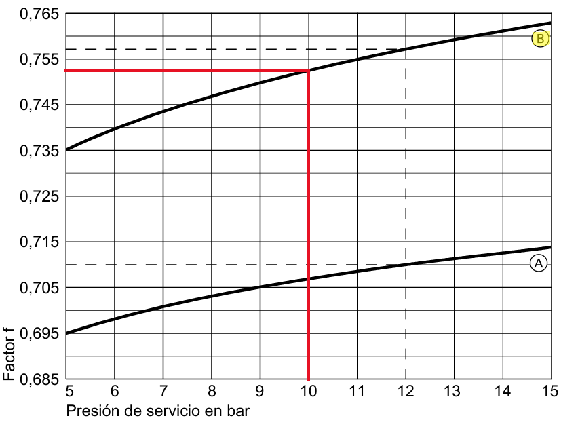
\includegraphics[width=0.75\textwidth]{Figuras/seleccion_factor_f.pdf}
	\caption{Gráfica para la determinación del factor $f$ en función de la presión de vapor}
	\label{fig:seleccion-factor-f}
\end{figure}

Para una presión de 10~bar(a), el factor $f$ obtenido de la gráfica es aproximadamente $f = 0{,}753$~kW/(kg/h). La potencia térmica estimada mediante este método es:

\begin{equation}
	P_f = f \cdot Q = 0{,}753 \times 5400 = 4066 \ \text{kW}
	\label{eq:potencia-factor-f}
\end{equation}

La diferencia entre ambos métodos (4217~kW frente a 4066~kW) se debe a que el factor $f$ corresponde típicamente a vapor saturado, mientras que el balance entálpico considera las condiciones reales de vapor sobrecalentado. El método del balance entálpico proporciona un resultado más preciso y conservador para la instalación analizada.

\paragraph{Margen de reserva de la instalación}

La caldera Viessmann VITOMAX 100-HS seleccionada tiene una capacidad nominal de 5400~kg/h, valor que supera el caudal de diseño calculado de 5078,4~kg/h. La \tabref{tab:margen-reserva-instalacion} presenta la comparación entre la demanda de la instalación y la capacidad disponible de la caldera.

\begin{table}[H]
	\centering
	\caption{Comparación entre demanda y capacidad de la caldera}
	\label{tab:margen-reserva-instalacion}
	\begin{tabular}{lccc}
		\toprule
		\textbf{Parámetro}              & \textbf{Demanda} & \textbf{Capacidad caldera} & \textbf{Margen} \\
		\midrule
		Caudal nominal (sin $K$)        & 4416~kg/h        & 5400~kg/h                  & +22,3\%         \\
		Caudal de diseño ($K = 1{,}15$) & 5078,4~kg/h      & 5400~kg/h                  & +6,3\%          \\
		Potencia térmica                & $\sim$3449~kW    & $\sim$4217~kW              & +22,3\%         \\
		\bottomrule
	\end{tabular}
\end{table}

El margen de reserva del 6,3\% sobre el caudal de diseño (equivalente al 22,3\% sobre el caudal nominal de los consumidores) garantiza la capacidad de la caldera para satisfacer la demanda en condiciones normales de operación, incluyendo las pérdidas por fugas consideradas en el factor $K$.

El margen de reserva calculado se considera adecuado para una instalación industrial de estas características, proporcionando flexibilidad operativa ante posibles variaciones de carga sin sobredimensionar excesivamente el equipo de generación. La capacidad excedente permite, además, absorber picos puntuales de demanda que pudieran producirse durante maniobras de puesta en marcha de los consumidores, aunque estos transitorios no han sido objeto de análisis específico en el presente proyecto.

% =============================================================================
% Sección 2.1.4: Selección de la caldera de vapor (Vitomax) y condiciones de salida
% Generado por latex-writer | Fecha: 2026-03-25
% =============================================================================

\subsubsection{Selección de la caldera de vapor y condiciones de salida}
\label{subsubsec:seleccion-caldera-vitomax}

La selección de la caldera constituye una decisión de diseño fundamental que condiciona las prestaciones de toda la instalación de vapor. El equipo seleccionado debe satisfacer simultáneamente los requerimientos de caudal, presión y temperatura demandados por los consumidores, garantizando además un margen de reserva adecuado para absorber variaciones de carga y pérdidas inherentes al sistema.

\paragraph{Criterios de selección}

La determinación de la caldera apropiada para la instalación se ha realizado considerando los siguientes criterios técnicos:

\begin{enumerate}[label=\arabic*., leftmargin=2em]
	\item \textbf{Capacidad de producción:} El caudal nominal de la caldera debe ser igual o superior al caudal de diseño calculado (5078,4~kg/h), correspondiente al caudal de los consumidores mayorado por el factor de seguridad $K = 1{,}15$.
	\item \textbf{Presión de trabajo:} La presión de diseño de la caldera debe compensar las pérdidas de carga en la red de distribución, garantizando la presión mínima requerida en todos los puntos de consumo.
	\item \textbf{Tipo de vapor:} Capacidad de generar vapor sobrecalentado a 220~°C para minimizar la formación de condensados durante el transporte.
	\item \textbf{Tecnología y eficiencia:} Caldera pirotubular de alta eficiencia, diseñada para operación continua en aplicaciones industriales.
\end{enumerate}

\paragraph{Determinación de la presión de diseño}

La presión mínima requerida en la caldera se determina a partir de la presión máxima demandada por los consumidores, adicionando las pérdidas de carga previstas en la red de distribución. El proceso de cálculo se desarrolla de la siguiente manera:

\begin{itemize}[leftmargin=2em]
	\item Presión máxima requerida por los consumidores (C2, C3, C4): 7~bar(g)
	\item Pérdida de carga admisible en la red: 1~bar
	\item Presión mínima en caldera: $P_{\text{caldera}} = 7 + 1 = 8$~bar(g)
	\item Corrección por altitud (700~m, $P_{\text{atm}} = 0{,}932$~bar): $P_{\text{abs}} = 8 + 0{,}932 \approx 9$~bar(a)
	\item Ajuste según disponibilidad comercial: 10~bar(g)
\end{itemize}

La presión absoluta de trabajo resulta ser 10~bar(a), equivalente a 9,068~bar(g) una vez considerada la corrección por altitud del emplazamiento.

\paragraph{Caldera seleccionada}

Tras el análisis del catálogo del fabricante Viessmann, se ha seleccionado la caldera VITOMAX 100-HS modelo M33A, cuyas especificaciones técnicas satisfacen los requerimientos de la instalación. La \tabref{tab:especificaciones-caldera-vitomax} recoge las características principales del equipo.

\begin{table}[H]
	\centering
	\caption{Especificaciones técnicas de la caldera Viessmann VITOMAX 100-HS M33A}
	\label{tab:especificaciones-caldera-vitomax}
	\begin{tabular}{lcc}
		\toprule
		\textbf{Parámetro}                   & \textbf{Valor} & \textbf{Unidad} \\
		\midrule
		Fabricante                           & Viessmann      & ---             \\
		Serie                                & VITOMAX 100-HS & ---             \\
		Modelo                               & M33A           & ---             \\
		Tipo                                 & Pirotubular    & ---             \\
		Capacidad de producción de vapor     & 5400           & kg/h            \\
		Presión de diseño                    & 10             & bar(g)          \\
		Presión absoluta de trabajo          & 10             & bar(a)          \\
		Temperatura de salida del vapor      & 220            & °C              \\
		Tipo de vapor                        & Sobrecalentado & ---             \\
		Temperatura del agua de alimentación & 15             & °C              \\
		\bottomrule
	\end{tabular}
\end{table}

\paragraph{Justificación técnica de la selección}

La elección de la caldera VITOMAX 100-HS modelo M33A se justifica por las siguientes razones técnicas:

\begin{enumerate}[label=\arabic*., leftmargin=2em]
	\item \textbf{Capacidad adecuada:} El caudal comercial de 5400~kg/h es el inmediatamente superior al caudal de diseño calculado de 5078,4~kg/h, proporcionando un margen de reserva del 6,3\% adicional.
	\item \textbf{Presión suficiente:} La presión de diseño de 10~bar(g) garantiza que, tras las pérdidas de carga en la red (máximo 0,38~bar hasta el consumidor más desfavorable C4), todos los puntos de consumo recibirán vapor a la presión requerida.
	\item \textbf{Tecnología apropiada:} La caldera pirotubular de alta eficiencia está diseñada para operación continua en aplicaciones industriales, con alta fiabilidad y bajo mantenimiento.
	\item \textbf{Disponibilidad comercial:} El modelo existe en el catálogo actual del fabricante Viessmann, garantizando el suministro de repuestos y servicio técnico.
\end{enumerate}

La \tabref{tab:comparacion-demanda-caldera} presenta la comparación detallada entre la demanda de la instalación y la capacidad de la caldera seleccionada.

\begin{table}[H]
	\centering
	\caption{Comparación entre la demanda de la instalación y la capacidad de la caldera}
	\label{tab:comparacion-demanda-caldera}
	\begin{tabular}{lcc}
		\toprule
		\textbf{Concepto}                   & \textbf{Valor} & \textbf{Unidad} \\
		\midrule
		Caudal nominal total (C1+C2+C3+C4)  & 4416           & kg/h            \\
		Factor de seguridad por fugas ($K$) & 1,15           & ---             \\
		Caudal de diseño                    & 5078,4         & kg/h            \\
		Caudal comercial de la caldera      & 5400           & kg/h            \\
		Margen de reserva disponible        & 321,6          & kg/h            \\
		Margen de reserva porcentual        & 6,3            & \%              \\
		\bottomrule
	\end{tabular}
\end{table}

\paragraph{Propiedades termodinámicas del vapor a la salida}

El vapor generado por la caldera VITOMAX 100-HS abandona el equipo en condiciones de sobrecalentamiento. Las propiedades termodinámicas del vapor a la salida de la caldera se recogen en la \tabref{tab:condiciones-salida-caldera}.

\begin{table}[H]
	\centering
	\caption{Condiciones del vapor a la salida de la caldera}
	\label{tab:condiciones-salida-caldera}
	\begin{tabular}{lcc}
		\toprule
		\textbf{Propiedad}          & \textbf{Valor} & \textbf{Unidad} \\
		\midrule
		Presión absoluta            & 10             & bar(a)          \\
		Presión manométrica         & 9,068          & bar(g)          \\
		Temperatura del vapor       & 220            & °C              \\
		Estado del vapor            & Sobrecalentado & ---             \\
		Temperatura de saturación   & 180            & °C              \\
		Grado de sobrecalentamiento & $\sim$40       & °C              \\
		Entalpía específica ($h_v$) & 2874           & kJ/kg           \\
		Densidad ($\rho$)           & 4,85           & kg/m³           \\
		Calor específico ($c_p$)    & 2,08           & kJ/(kg·K)       \\
		\bottomrule
	\end{tabular}
\end{table}

El grado de sobrecalentamiento de aproximadamente 40~°C (diferencia entre la temperatura real del vapor, 220~°C, y la temperatura de saturación a 10~bar(a), aproximadamente 180~°C) proporciona un margen térmico adecuado para prevenir la condensación prematura del vapor durante su transporte a través de la red de distribución.

\paragraph{Cálculo de la potencia térmica}

La potencia térmica de la caldera se determina mediante el balance entálpico entre las condiciones del vapor generado y el agua de alimentación:

\begin{equation}
	P = \dot{m} \cdot (h_v - h_w)
	\label{eq:potencia-termica-caldera}
\end{equation}

\noindent donde $\dot{m}$ es el caudal másico (kg/s), $h_v$ es la entalpía del vapor sobrecalentado (kJ/kg) y $h_w$ es la entalpía del agua de alimentación (kJ/kg).

Sustituyendo los valores correspondientes a las condiciones de operación:

\begin{equation}
	P = \frac{5400}{3600} \times (2874 - 62{,}7) = 1{,}5 \times 2811{,}3 = 4217 \ \text{kW}
	\label{eq:potencia-caldera-calculada}
\end{equation}

La potencia térmica de 4217~kW corresponde a la capacidad nominal de la caldera operando a su caudal máximo de 5400~kg/h. Para el caudal nominal de los consumidores (4416~kg/h, sin considerar el factor $K$), la potencia requerida sería:

\begin{equation}
	P_{\text{nominal}} = \frac{4416}{3600} \times 2811{,}3 = 1{,}227 \times 2811{,}3 = 3449 \ \text{kW}
	\label{eq:potencia-nominal-consumidores}
\end{equation}

La \tabref{tab:resumen-potencias-caldera} presenta el resumen de las potencias térmicas calculadas para los distintos escenarios de operación.

\begin{table}[H]
	\centering
	\caption{Resumen de potencias térmicas según escenario de operación}
	\label{tab:resumen-potencias-caldera}
	\begin{tabular}{lccc}
		\toprule
		\textbf{Escenario}            & \textbf{Caudal [kg/h]} & \textbf{Caudal [kg/s]} & \textbf{Potencia [kW]} \\
		\midrule
		Caudal nominal consumidores   & 4416                   & 1,227                  & 3449                   \\
		Caudal de diseño ($K=1{,}15$) & 5078,4                 & 1,411                  & 3966                   \\
		Capacidad nominal caldera     & 5400                   & 1,500                  & 4217                   \\
		\bottomrule
	\end{tabular}
\end{table}

\paragraph{Representación gráfica}

La \figref{fig:ficha-caldera-vitomax} muestra un extracto de la ficha técnica del fabricante correspondiente a la caldera seleccionada.

\begin{figure}[H]
	\centering
	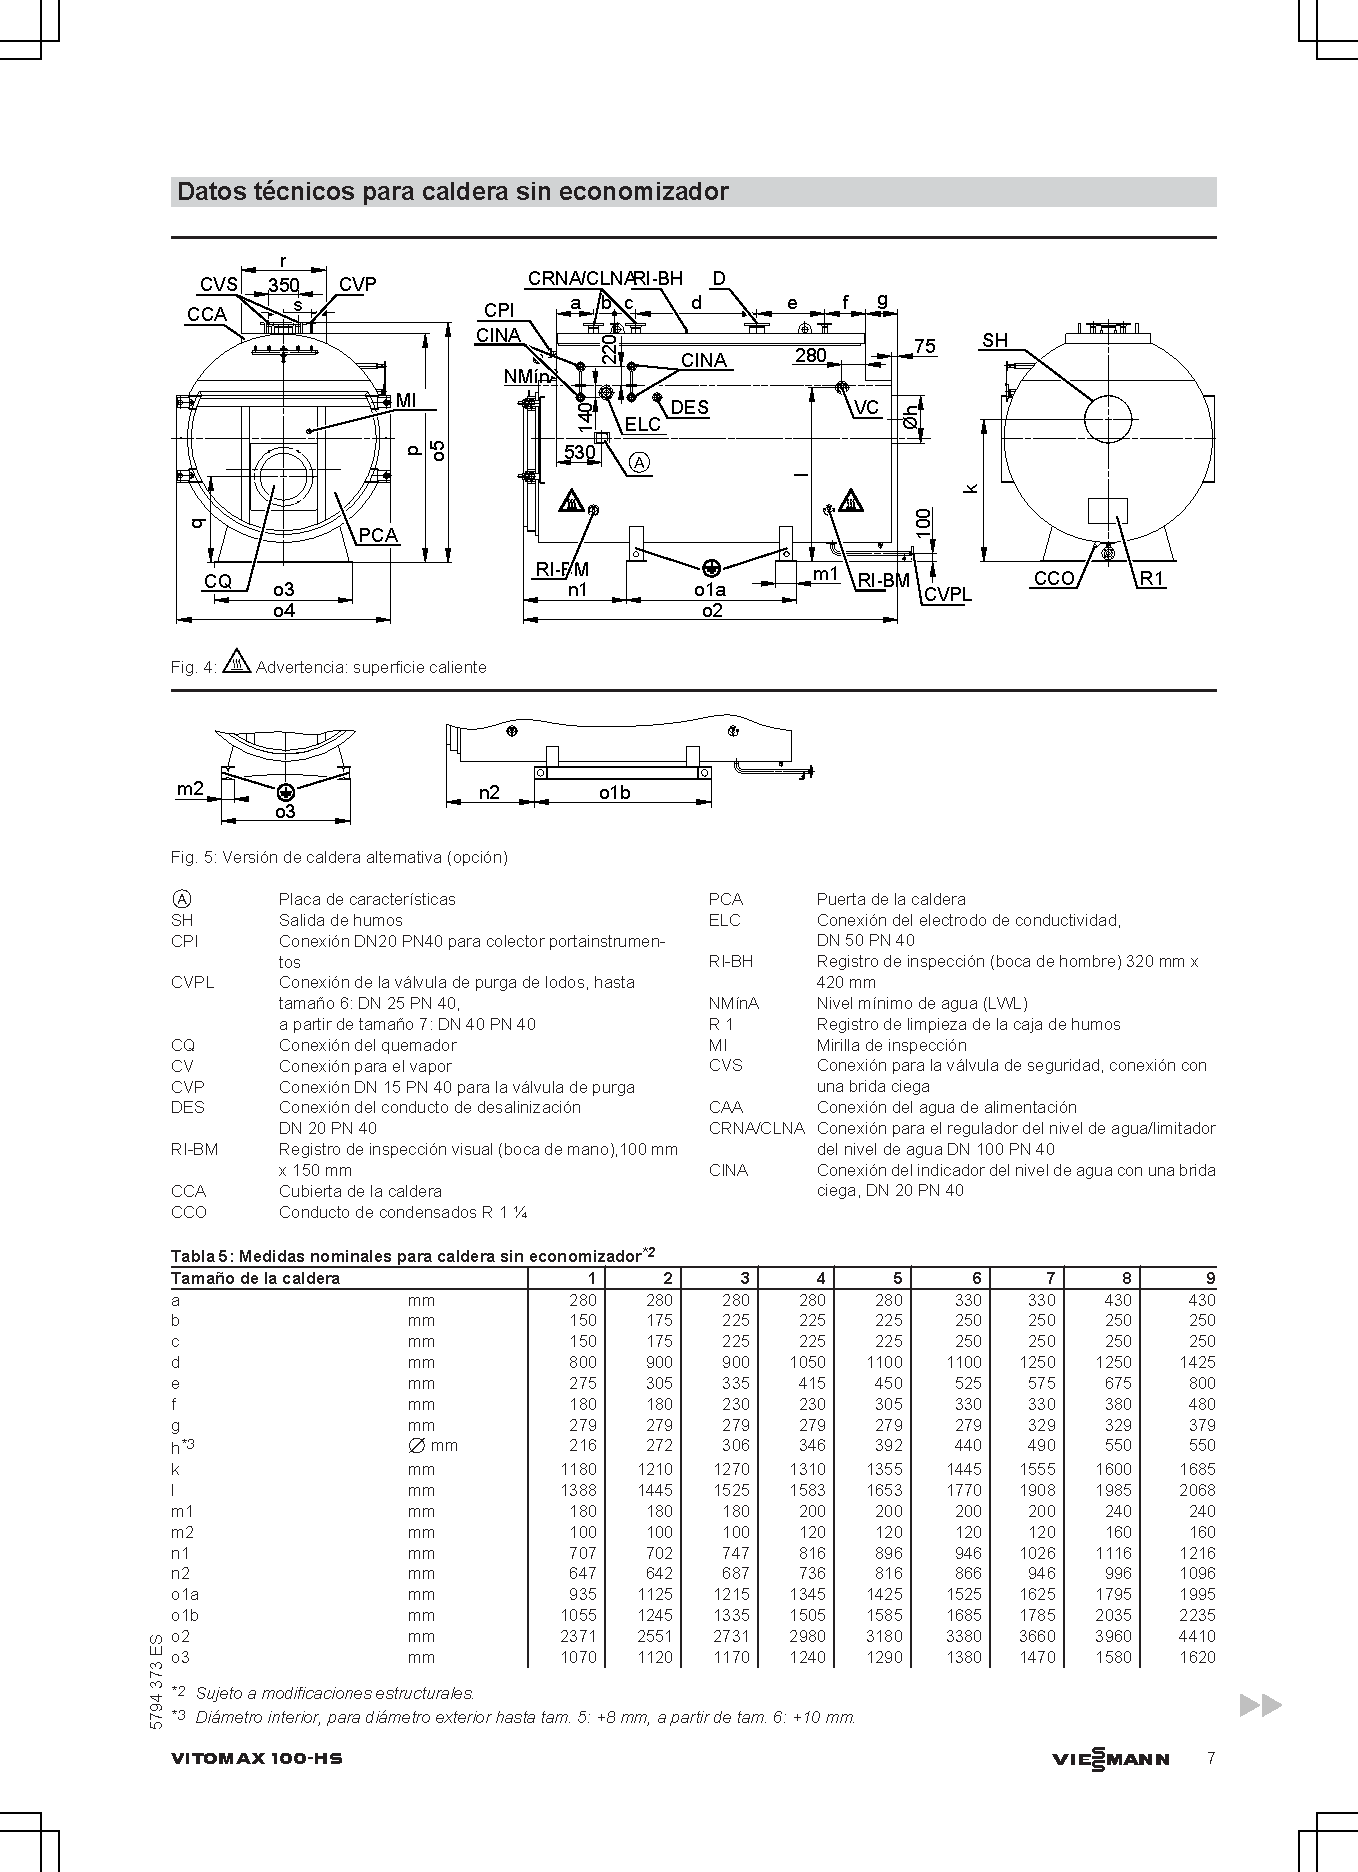
\includegraphics[trim={3cm 21cm 15.3cm 4.2cm}, clip, keepaspectratio, width=0.45\textwidth]{Figuras/Vitomax_100HS_33-A.pdf}
	\caption{Esquema de la caldera Viessmann VITOMAX 100-HS M33A. Fuente: Catálogo Viessmann}
	\label{fig:ficha-caldera-vitomax}
\end{figure}

Las condiciones de salida de la caldera (10~bar(a), 220~°C, vapor sobrecalentado) constituyen el punto de partida para el dimensionamiento de la red de distribución de vapor que se desarrolla en las secciones subsiguientes de la presente memoria técnica.

% =============================================================================
% Sección 2.2: Dimensionado Hidráulico de la Red de Vapor
% Sección 2.2.1: Criterios de dimensionado
% Generado por latex-writer | Fecha: 2026-03-25
% =============================================================================

\subsection{Dimensionado Hidráulico de la Red de Vapor}
\label{subsec:dimensionado-red-vapor}

El dimensionado hidráulico de la red de distribución de vapor constituye una etapa fundamental del proyecto, cuyo objetivo es determinar los diámetros de tubería apropiados para cada tramo de la instalación. El proceso de dimensionado debe garantizar que el sistema opere dentro de límites técnicos y económicos aceptables, asegurando el suministro de vapor a todos los puntos de consumo con las condiciones de presión y caudal requeridas.

El dimensionado se aborda mediante un procedimiento sistemático que parte de los criterios de diseño establecidos en la normativa de referencia, aplica las ecuaciones fundamentales de la mecánica de fluidos y verifica el cumplimiento de las restricciones impuestas. Los criterios adoptados buscan un equilibrio entre el coste de la instalación (diámetros pequeños) y las pérdidas de carga asociadas (diámetros grandes), optimizando el funcionamiento global del sistema.

\subsubsection{Criterios de dimensionado}
\label{subsubsec:criterios-dimensionado}

El dimensionado de las tuberías de vapor se fundamenta en tres criterios principales: la velocidad máxima admisible del fluido, la caída de presión total permitida en la red y la rugosidad del material de las tuberías. Estos criterios, establecidos a partir de la normativa y guías técnicas de referencia (RITE, Manual EREN, Guía Spirax Sarco), definen las restricciones que debe cumplir el diseño para garantizar un funcionamiento seguro y eficiente de la instalación.

\paragraph{Criterio de velocidad}

La velocidad del vapor en el interior de las tuberías constituye el parámetro de control principal en el dimensionado de redes de distribución. Una velocidad excesivamente alta provoca efectos indeseables que comprometen la integridad y el funcionamiento del sistema:

\begin{itemize}[leftmargin=2em]
	\item \textbf{Erosión en codos y accesorios:} Las partículas de condensado arrastradas por el vapor a alta velocidad impactan contra las paredes internas de los accesorios, provocando un desgaste progresivo del material.
	\item \textbf{Incremento del nivel de ruido:} Velocidades elevadas generan turbulencias y vibraciones que se traducen en niveles de ruido inaceptables en entornos industriales.
	\item \textbf{Mayores pérdidas de carga:} La pérdida de presión por fricción es proporcional al cuadrado de la velocidad, por lo que velocidades altas incrementan significativamente las pérdidas energéticas.
	\item \textbf{Riesgo de vibraciones y fatiga mecánica:} Las fluctuaciones de presión asociadas a flujos turbulentos a alta velocidad pueden inducir vibraciones en las tuberías y sus soportes, acelerando la fatiga del material.
\end{itemize}

Para la presente instalación se ha adoptado una \textbf{velocidad de diseño de aproximadamente 20~m/s}, valor que permite compatibilizar un diámetro de tubería económicamente razonable con pérdidas de carga moderadas y un funcionamiento hidráulico adecuado. Este valor se encuentra dentro del rango recomendado por las guías técnicas de referencia para líneas de vapor industrial.

La \tabref{tab:velocidades-recomendadas} presenta los rangos de velocidad recomendados según el tipo de aplicación y las condiciones de presión del vapor, de acuerdo con las guías técnicas de Spirax Sarco y el Manual EREN.

\begin{table}[H]
	\centering
	\caption{Velocidades recomendadas del vapor según tipo de aplicación y presión}
	\label{tab:velocidades-recomendadas}
	\begin{tabular}{lc}
		\toprule
		\textbf{Tipo de línea / Condición de presión} & \textbf{Velocidad recomendada [m/s]} \\
		\midrule
		Líneas principales (vapor saturado)           & 25 -- 40                             \\
		Presión $<$ 2~bar                             & 30                                   \\
		Presión 2 -- 5~bar                            & 35                                   \\
		Presión 5 -- 10~bar                           & 40                                   \\
		Presión 10 -- 25~bar                          & 50                                   \\
		Líneas de gran longitud                       & 15                                   \\
		Derivaciones cortas                           & 25 -- 35                             \\
		\bottomrule
	\end{tabular}
\end{table}

Para la presente instalación, que opera a una presión de 10~bar(a) con tramos de longitud considerable (hasta 223,74~m hasta el consumidor más alejado C4), la velocidad de diseño de 20~m/s representa un valor conservador que prioriza la minimización de pérdidas de carga. Como criterio de seguridad adicional, se establece una \textbf{velocidad máxima absoluta de 30~m/s} que no debe superarse en ningún tramo de la instalación.

\paragraph{Criterio de caída de presión}

El segundo criterio de dimensionado establece la pérdida de carga máxima admisible en la red de distribución. Este límite garantiza que todos los puntos de consumo reciban vapor a la presión mínima requerida, considerando la presión disponible a la salida de la caldera.

Para la presente instalación se ha adoptado un criterio de \textbf{pérdida de carga máxima de 1~bar} por recorrido completo desde la caldera hasta el consumidor más desfavorable. Este criterio permite establecer la presión mínima requerida en la caldera:

\begin{equation}
	P_{\text{caldera}} = P_{\text{máx,consumidor}} + \Delta P_{\text{red}} = 7 + 1 = 8 \ \text{bar(g)}
	\label{eq:presion-minima-caldera}
\end{equation}

La caldera seleccionada opera a una presión efectiva de 9,068~bar(g), lo que proporciona un margen disponible para pérdidas de carga de:

\begin{equation}
	\Delta P_{\text{disponible}} = P_{\text{caldera}} - P_{\text{máx,consumidor}} = 9{,}068 - 7 = 2{,}068 \ \text{bar}
	\label{eq:margen-presion-disponible}
\end{equation}

Este margen, superior al criterio de diseño de 1~bar, proporciona una reserva de presión que permite absorber variaciones de carga y posibles obstrucciones parciales en la red sin comprometer el suministro a los consumidores.

Las pérdidas de carga en la red se calculan mediante la ecuación de \textbf{Darcy-Weisbach}, expresión fundamental de la mecánica de fluidos para el cálculo de pérdidas por fricción en conductos:

\begin{equation}
	\Delta P = f \cdot \frac{L}{D} \cdot \frac{\rho \cdot v^2}{2}
	\label{eq:darcy-weisbach}
\end{equation}

\noindent donde:
\begin{itemize}[leftmargin=2em, label={}]
	\item $\Delta P$ = pérdida de presión por fricción [Pa]
	\item $f$ = factor de fricción de Darcy [adimensional]
	\item $L$ = longitud total de cálculo [m]
	\item $D$ = diámetro interior de la tubería [m]
	\item $\rho$ = densidad del vapor [kg/m³]
	\item $v$ = velocidad del vapor [m/s]
\end{itemize}

El factor de fricción $f$ depende del número de Reynolds y de la rugosidad relativa de la tubería ($\varepsilon/D$), obteniéndose mediante el diagrama de Moody o mediante correlaciones empíricas como la ecuación de Colebrook-White para régimen turbulento.

\paragraph{Rugosidad y material de tuberías}

El tercer criterio de dimensionado hace referencia a las características del material de las tuberías, que determinan la rugosidad superficial y, por tanto, las pérdidas de carga por fricción.

Para la presente instalación se ha seleccionado \textbf{tubería de acero al carbono sin soldadura}, material de uso generalizado en redes de vapor industrial por su resistencia mecánica, durabilidad y coste competitivo. Las tuberías se dimensionan de acuerdo con las siguientes normas técnicas:

\begin{itemize}[leftmargin=2em]
	\item \textbf{DIN 2448:} Norma europea para tuberías de acero sin soldadura, de aplicación preferente para los diámetros nominales empleados en la instalación (DN~50 a DN~150).
	\item \textbf{Sistema Schedule (API):} Sistema americano que define el espesor de pared en función de la presión de trabajo. Se adopta Schedule~40 como estándar de diseño.
\end{itemize}

La \textbf{rugosidad absoluta} ($\varepsilon$) del acero comercial nuevo se sitúa en el rango de 0,045 a 0,05~mm. Para los cálculos de la presente instalación se adopta el valor:

\begin{equation}
	\varepsilon = 0{,}045 \ \text{mm}
	\label{eq:rugosidad-acero}
\end{equation}

La \tabref{tab:rugosidades-materiales} presenta los valores de rugosidad absoluta para diferentes materiales de tubería, permitiendo contextualizar el valor adoptado para el acero comercial.

\begin{table}[H]
	\centering
	\caption{Rugosidad absoluta de diferentes materiales de tubería}
	\label{tab:rugosidades-materiales}
	\begin{tabular}{lc}
		\toprule
		\textbf{Material}     & \textbf{Rugosidad $\varepsilon$ [mm]} \\
		\midrule
		Acero comercial nuevo & 0,045 -- 0,05                         \\
		Acero galvanizado     & 0,15                                  \\
		Acero oxidado         & 0,15 -- 0,25                          \\
		Fundición nueva       & 0,25 -- 0,50                          \\
		Cobre / Latón         & 0,0015 -- 0,002                       \\
		PVC / Plásticos       & 0,0015 -- 0,007                       \\
		\bottomrule
	\end{tabular}
\end{table}

La \tabref{tab:diam_tuberias_norma_DIN} presenta los diámetros normalizados según la norma DIN~2448, que serán utilizados para la selección de tuberías comerciales en cada tramo de la instalación.

\paragraph{Ecuaciones fundamentales de dimensionado}

El dimensionado de cada tramo de la red se realiza mediante la aplicación de las ecuaciones fundamentales de la mecánica de fluidos, partiendo del caudal demandado y la velocidad objetivo para determinar el diámetro teórico, que posteriormente se ajusta al diámetro comercial normalizado.

La \textbf{ecuación de continuidad} permite calcular el diámetro teórico de la tubería a partir del caudal volumétrico y la velocidad de diseño:

\begin{equation}
	D = \sqrt{\frac{4 \cdot \dot{V}}{\pi \cdot C}}
	\label{eq:continuidad-diametro}
\end{equation}

\noindent donde:
\begin{itemize}[leftmargin=2em, label={}]
	\item $D$ = diámetro interior teórico [m]
	\item $\dot{V}$ = caudal volumétrico [m³/s]
	\item $C$ = velocidad objetivo [m/s]
\end{itemize}

El caudal volumétrico se obtiene a partir del caudal másico y la densidad del vapor:

\begin{equation}
	\dot{V} = \frac{\dot{m}}{\rho}
	\label{eq:caudal-volumetrico}
\end{equation}

Para el cálculo de las pérdidas de carga, la \textbf{longitud de cálculo} debe incluir tanto la longitud real de la tubería como las longitudes equivalentes de los accesorios presentes en el tramo:

\begin{equation}
	L_{\text{cálculo}} = L_{\text{real}} + L_{\text{eq}}
	\label{eq:longitud-calculo}
\end{equation}

Las longitudes equivalentes de los accesorios se expresan habitualmente como múltiplos del diámetro interior de la tubería ($L_e/D$). La \tabref{tab:longitudes-equivalentes} recoge los valores adoptados para los accesorios más comunes, según el Manual EREN.

\begin{table}[H]
	\centering
	\caption{Longitudes equivalentes de accesorios en función del diámetro}
	\label{tab:longitudes-equivalentes}
	\begin{tabular}{lc}
		\toprule
		\textbf{Accesorio}      & \textbf{$L_e/D$} \\
		\midrule
		Codo 90° radio medio    & 26               \\
		Codo 90° radio estándar & 32               \\
		T (paso recto)          & 60               \\
		T (derivación)          & 90               \\
		Válvula de compuerta    & 13               \\
		Válvula de globo        & 340              \\
		\bottomrule
	\end{tabular}
\end{table}

La \tabref{tab:perdidas_carga_accesorios} proporciona información adicional sobre pérdidas de carga en accesorios para diferentes diámetros de tubería.

\paragraph{Propiedades del vapor para el cálculo}

Las propiedades termodinámicas del vapor sobrecalentado a las condiciones de operación (10~bar(a), 220~°C) que se emplean en los cálculos de dimensionado son las siguientes:

\begin{table}[H]
	\centering
	\caption{Propiedades del vapor para cálculos de dimensionado}
	\label{tab:propiedades-vapor-dimensionado}
	\begin{tabular}{lccc}
		\toprule
		\textbf{Propiedad}    & \textbf{Símbolo} & \textbf{Valor}          & \textbf{Unidad} \\
		\midrule
		Densidad              & $\rho$           & 4,85                    & kg/m³           \\
		Viscosidad dinámica   & $\mu$            & 1,74 $\times$ 10$^{-5}$ & Pa·s            \\
		Viscosidad cinemática & $\nu$            & 3,59 $\times$ 10$^{-6}$ & m²/s            \\
		\bottomrule
	\end{tabular}
\end{table}

La \tabref{tab:resumen-criterios-dimensionado} presenta un resumen de los criterios de dimensionado adoptados para la red de distribución de vapor.

\begin{table}[H]
	\centering
	\caption{Resumen de criterios de dimensionado de la red de vapor}
	\label{tab:resumen-criterios-dimensionado}
	\begin{tabular}{lcc}
		\toprule
		\textbf{Criterio}                  & \textbf{Valor adoptado} & \textbf{Fuente}     \\
		\midrule
		Velocidad de diseño                & $\sim$20~m/s            & EREN, Spirax Sarco  \\
		Velocidad máxima absoluta          & 30~m/s                  & EREN                \\
		Pérdida de carga máxima admisible  & 1~bar                   & Criterio de diseño  \\
		Material de tuberías               & Acero al carbono        & DIN 2448            \\
		Rugosidad absoluta ($\varepsilon$) & 0,045~mm                & Tablas normalizadas \\
		Schedule de tubería                & Schedule 40             & API                 \\
		\bottomrule
	\end{tabular}
\end{table}

Estos criterios de dimensionado constituyen la base para el cálculo detallado de cada tramo de la red de distribución de vapor, que se desarrolla en las subsecciones siguientes de la presente memoria técnica.

% =============================================================================
% Sección 2.2.2: Cálculo de longitudes equivalentes por accesorios
% Generado por latex-writer | Fecha: 2026-03-25
% =============================================================================

\subsubsection{Cálculo de longitudes equivalentes por accesorios}
\label{subsubsec:longitudes-equivalentes-accesorios}

El cálculo de las pérdidas de carga en una red de distribución de vapor no puede limitarse a las pérdidas por fricción en los tramos rectos de tubería. Los accesorios presentes en la instalación ---codos, derivaciones en T, válvulas y demás elementos--- introducen perturbaciones en el flujo que se traducen en pérdidas de carga adicionales. El método de las longitudes equivalentes permite cuantificar estas pérdidas expresándolas como una longitud ficticia de tubería recta que produciría la misma caída de presión.

\paragraph{Concepto de longitud equivalente}

La longitud equivalente de un accesorio representa la longitud de tubería recta, del mismo diámetro, que ocasionaría una pérdida de carga idéntica a la producida por dicho accesorio. Este concepto simplifica significativamente el cálculo de pérdidas de carga, ya que permite sumar todas las longitudes (reales y equivalentes) y aplicar una única expresión de pérdida por fricción al conjunto.

Los valores de longitud equivalente se expresan habitualmente como múltiplos del diámetro interior de la tubería, mediante el coeficiente adimensional $L_e/D$. La longitud equivalente absoluta de cada accesorio se obtiene multiplicando este coeficiente por el diámetro interior del tramo correspondiente:

\begin{equation}
	L_{e,i} = \left(\frac{L_e}{D}\right)_i \times D_{\text{interior}}
	\label{eq:longitud-equivalente-accesorio}
\end{equation}

\noindent donde $L_{e,i}$ es la longitud equivalente del accesorio $i$ en metros, $(L_e/D)_i$ es el coeficiente adimensional del accesorio y $D_{\text{interior}}$ es el diámetro interior de la tubería en metros.

La longitud equivalente total de un tramo se calcula sumando las contribuciones de todos los accesorios presentes:

\begin{equation}
	L_{\text{eq}} = \sum_{i=1}^{n} \left(\frac{L_e}{D}\right)_i \times D_{\text{interior}}
	\label{eq:longitud-equivalente-total}
\end{equation}

Finalmente, la longitud de cálculo empleada en la ecuación de Darcy-Weisbach (\autoref{eq:darcy-weisbach}) resulta de la suma de la longitud real del tramo y su longitud equivalente total:

\begin{equation}
	L_{\text{cálculo}} = L_{\text{real}} + L_{\text{eq}}
	\label{eq:longitud-calculo-total}
\end{equation}

\paragraph{Coeficientes de pérdidas en accesorios}

Los coeficientes $L_e/D$ dependen fundamentalmente de la geometría del accesorio y del régimen de flujo. La \tabref{tab:coeficientes-LeD-completa} presenta los valores adoptados para los accesorios más habituales en instalaciones de vapor, de acuerdo con el Manual Técnico de Diseño y Cálculo de Redes de Vapor (EREN, Junta de Castilla y León, 2010).

\begin{table}[H]
	\centering
	\caption{Coeficientes $L_e/D$ para accesorios en líneas de vapor}
	\label{tab:coeficientes-LeD-completa}
	\begin{tabular}{lc}
		\toprule
		\textbf{Accesorio}                                 & \textbf{$L_e/D$} \\
		\midrule
		Codo 45°                                           & 15               \\
		Codo 90° radio estándar ($R \approx 1 \cdot D$)    & 32               \\
		Codo 90° radio mediano ($R \approx 1{,}5 \cdot D$) & 26               \\
		Codo 90° radio grande                              & 20               \\
		Codo 90° en escuadra                               & 60               \\
		Codo 180° (retorno)                                & 75               \\
		Codo 180° radio mediano                            & 50               \\
		T (paso recto)                                     & 60               \\
		T (derivación)                                     & 90               \\
		Válvula de compuerta (abierta)                     & 7                \\
		Válvula de asiento/globo (abierta)                 & 300              \\
		Válvula angular (abierta)                          & 170              \\
		Válvula de esfera                                  & 3                \\
		Acoplamiento                                       & despreciable     \\
		Unión                                              & despreciable     \\
		\bottomrule
	\end{tabular}
\end{table}

La \figref{fig:tabla-perdidas-accesorios} muestra la tabla de referencia del Manual EREN con los valores de $L_e/D$ para diferentes accesorios y condiciones de instalación.

\begin{figure}[H]
	\centering
	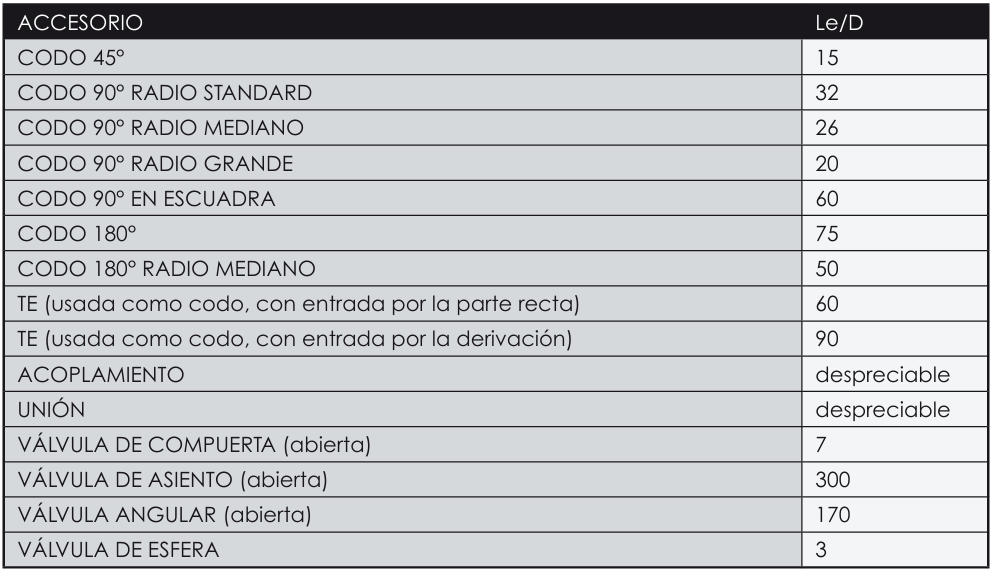
\includegraphics[width=0.85\textwidth]{Figuras/perdidas_carga_accesorios.png}
	\caption{Pérdidas de carga en accesorios expresadas como $L_e/D$. Fuente: Manual EREN (2010)}
	\label{fig:tabla-perdidas-accesorios}
\end{figure}

\paragraph{Selección del tipo de codo}

Para la presente instalación se han seleccionado \textbf{codos de radio mediano} ($R \approx 1{,}5 \cdot D$) con un coeficiente $L_e/D = 26$. Esta elección se justifica por las siguientes ventajas técnicas frente al codo de radio estándar:

\begin{enumerate}[label=\arabic*., leftmargin=2em]
	\item \textbf{Reducción de pérdidas de carga:} El codo de radio mediano presenta un coeficiente $L_e/D = 26$, frente a los 32 del codo de radio estándar. Esta diferencia supone una reducción de aproximadamente el 18\% en las pérdidas locales generadas por cada codo.
	\item \textbf{Mejora del perfil de velocidades:} El mayor radio de curvatura reduce las turbulencias en el interior del codo, mejorando el perfil de velocidades aguas abajo y minimizando los efectos de erosión sobre las paredes internas.
	\item \textbf{Recomendación técnica:} Las guías de diseño de redes de vapor (EREN, Spirax Sarco) recomiendan el uso de codos de radio mediano o grande en líneas principales, reservando los codos de radio estándar para derivaciones secundarias o restricciones de espacio.
\end{enumerate}

El incremento de coste asociado al codo de radio mediano queda justificado por la reducción de pérdidas de carga y la mejora de las condiciones de operación de la instalación.

\paragraph{Aplicación a los tramos del proyecto}

La \tabref{tab:accesorios-por-tramo} presenta el inventario de accesorios identificados en cada tramo de la red de distribución, junto con el diámetro de tanteo empleado para el cálculo de las longitudes equivalentes y los resultados obtenidos.

\begin{table}[H]
	\centering
	\caption{Accesorios por tramo y cálculo de longitudes equivalentes}
	\label{tab:accesorios-por-tramo}
	\begin{tabular}{lccccccc}
		\toprule
		\textbf{Tramo} & \textbf{$L_{\text{real}}$ [m]} & \textbf{Codos 90°} & \textbf{T (recta)} & \textbf{T (deriv.)} & \textbf{$D_{\text{tanteo}}$ [mm]} & \textbf{$L_{\text{eq}}$ [m]} & \textbf{$L_{\text{cálculo}}$ [m]} \\
		\midrule
		Caldera-P      & 12,74                          & 0                  & 0                  & 0                   & ---                               & 2,548                        & 15,288                            \\
		P-C$_1$        & 88,189                         & 2                  & 1                  & 0                   & 60                                & 9,24                         & 97,429                            \\
		P-S            & 106                            & 1                  & 0                  & 2                   & 120                               & 25,44                        & 131,44                            \\
		S-C$_2$        & 25                             & 0                  & 0                  & 0                   & ---                               & 5                            & 30                                \\
		S-T            & 60                             & 0                  & 1                  & 1                   & 120                               & 7,5                          & 78                                \\
		T-C$_3$        & 15                             & 0                  & 0                  & 0                   & ---                               & 3                            & 18                                \\
		T-C$_4$        & 45                             & 2                  & 1                  & 0                   & 100                               & 12,4                         & 57,4                              \\
		\bottomrule
	\end{tabular}
\end{table}

\paragraph{Criterio para tramos sin accesorios significativos}

En aquellos tramos donde no se han identificado accesorios relevantes (Caldera-P, S-C$_2$ y T-C$_3$), se aplica un criterio simplificado que consiste en mayorar la longitud real en un 20\%:

\begin{equation}
	L_{\text{eq}} = 0{,}20 \times L_{\text{real}}
	\label{eq:criterio-20-porciento}
\end{equation}

Este criterio, de uso habitual en la práctica industrial, permite considerar de forma aproximada las pérdidas asociadas a pequeños accesorios (uniones, soportes, ligeras curvaturas) que no se contabilizan individualmente. La \tabref{tab:tramos-criterio-20} detalla la aplicación de este criterio.

\begin{table}[H]
	\centering
	\caption{Aplicación del criterio del 20\% en tramos sin accesorios significativos}
	\label{tab:tramos-criterio-20}
	\begin{tabular}{lccc}
		\toprule
		\textbf{Tramo} & \textbf{$L_{\text{real}}$ [m]} & \textbf{$L_{\text{eq}} = 0{,}20 \times L_{\text{real}}$ [m]} & \textbf{$L_{\text{cálculo}}$ [m]} \\
			\midrule
		Caldera-P      & 12,74                          & 2,548                                                        & 15,288                            \\
		S-C$_2$        & 25                             & 5,000                                                        & 30,000                            \\
		T-C$_3$        & 15                             & 3,000                                                        & 18,000                            \\
		\bottomrule
	\end{tabular}
\end{table}

\paragraph{Ejemplo de cálculo: Tramo P-S}

A modo ilustrativo, se desarrolla el cálculo completo de la longitud equivalente para el tramo P-S, que conecta el punto de bifurcación principal con el nodo secundario S.

\textbf{Datos de partida:}
\begin{itemize}[leftmargin=2em]
	\item Longitud real del tramo: $L_{\text{real}} = 106$~m
	\item Codos 90° de radio mediano: 1 unidad ($L_e/D = 26$)
	\item T en derivación: 2 unidades ($L_e/D = 90$ cada una)
	\item Diámetro de tanteo: $D_{\text{tanteo}} = 120$~mm $= 0{,}120$~m
\end{itemize}

\textbf{Cálculo de la longitud equivalente:}

La suma de coeficientes $L_e/D$ de todos los accesorios del tramo es:

\begin{equation}
	\sum \left(\frac{L_e}{D}\right) = 1 \times 26 + 2 \times 90 = 26 + 180 = 206
	\label{eq:suma-LeD-PS}
\end{equation}

La longitud equivalente absoluta resulta:

\begin{equation}
	L_{\text{eq}} = 206 \times 0{,}120 = 24{,}72 \ \text{m} \approx 25{,}44 \ \text{m}
	\label{eq:Leq-PS}
\end{equation}

\textbf{Longitud de cálculo:}

\begin{equation}
	L_{\text{cálculo}} = L_{\text{real}} + L_{\text{eq}} = 106 + 25{,}44 = 131{,}44 \ \text{m}
	\label{eq:Lcalculo-PS}
\end{equation}

Este valor de 131,44~m será el empleado en la ecuación de Darcy-Weisbach para determinar la pérdida de carga en el tramo P-S.

\paragraph{Resumen de longitudes de cálculo}

La \tabref{tab:resumen-longitudes-calculo} presenta el resumen de las longitudes de cálculo obtenidas para todos los tramos de la red de distribución de vapor.

\begin{table}[H]
	\centering
	\caption{Resumen de longitudes de cálculo para la red de vapor}
	\label{tab:resumen-longitudes-calculo}
	\begin{tabular}{lcccl}
		\toprule
		\textbf{Tramo} & \textbf{$L_{\text{real}}$ [m]} & \textbf{$L_{\text{eq}}$ [m]} & \textbf{$L_{\text{cálculo}}$ [m]} & \textbf{Método} \\
		\midrule
		Caldera-P      & 12,74                          & 2,548                        & 15,288                            & Criterio 20\%   \\
		P-C$_1$        & 88,189                         & 9,24                         & 97,429                            & $L_e/D$         \\
		P-S            & 106                            & 25,44                        & 131,44                            & $L_e/D$         \\
		S-C$_2$        & 25                             & 5                            & 30                                & Criterio 20\%   \\
		S-T            & 60                             & 7,5                          & 78                                & $L_e/D$         \\
		T-C$_3$        & 15                             & 3                            & 18                                & Criterio 20\%   \\
		T-C$_4$        & 45                             & 12,4                         & 57,4                              & $L_e/D$         \\
		\midrule
		\textbf{Total} & \textbf{351,93}                & \textbf{65,13}               & \textbf{427,56}                   & ---             \\
		\bottomrule
	\end{tabular}
\end{table}

Las longitudes equivalentes calculadas representan un incremento medio del 18,5\% sobre las longitudes reales de la instalación. Este porcentaje se encuentra dentro del rango habitual para redes de vapor industrial con un número moderado de accesorios. Las longitudes de cálculo obtenidas serán empleadas en los cálculos de pérdida de carga que se desarrollan en las secciones posteriores de la presente memoria.

% =============================================================================
% Sección 2.2.3: Tramo 1 (Caldera-P)
% Generado por latex-writer | Fecha: 2026-03-25
% =============================================================================

\subsubsection{Tramo 1: Caldera-P}
\label{subsubsec:tramo1-caldera-p}

El Tramo~1 constituye la línea principal de salida de la caldera, conectando el equipo generador con el primer nodo de bifurcación (punto~P) de la red de distribución. Este tramo transporta el 100\% del caudal de vapor generado, por lo que su correcto dimensionamiento resulta crítico para el funcionamiento global de la instalación.

\paragraph{Datos de partida}

El tramo Caldera-P presenta las características geométricas y de operación recogidas en la \tabref{tab:datos-partida-tramo1}.

\begin{table}[H]
	\centering
	\caption{Datos de partida para el Tramo 1 (Caldera-P)}
	\label{tab:datos-partida-tramo1}
	\begin{tabular}{lcc}
		\toprule
		\textbf{Parámetro}   & \textbf{Valor}  & \textbf{Unidad} \\
		\midrule
		Identificación       & TR1 (Caldera-P) & ---             \\
		Longitud real        & 12,74           & m               \\
		Longitud equivalente & 2,548           & m               \\
		Longitud de cálculo  & 15,288          & m               \\
		Caudal másico        & 5400            & kg/h            \\
		Caudal másico        & 1,5             & kg/s            \\
		Presión de entrada   & 9,068           & bar(g)          \\
		Temperatura          & 220             & °C              \\
		Tipo de tramo        & Aéreo           & ---             \\
		\bottomrule
	\end{tabular}
\end{table}

Este tramo no presenta accesorios significativos (0~codos, 0~derivaciones en~T), por lo que la longitud equivalente se ha calculado aplicando el criterio del 20\% sobre la longitud real:

\begin{equation}
	L_{\text{eq}} = 0{,}20 \times L_{\text{real}} = 0{,}20 \times 12{,}74 = 2{,}548 \ \text{m}
	\label{eq:Leq-tramo1}
\end{equation}

Las propiedades del vapor sobrecalentado a las condiciones de operación (10~bar(a), 220~°C) se presentan en la \tabref{tab:propiedades-vapor-tramo1}.

\begin{table}[H]
	\centering
	\caption{Propiedades del vapor en el Tramo 1}
	\label{tab:propiedades-vapor-tramo1}
	\begin{tabular}{lccc}
		\toprule
		\textbf{Propiedad}    & \textbf{Símbolo} & \textbf{Valor}          & \textbf{Unidad} \\
		\midrule
		Densidad              & $\rho$           & 4,85                    & kg/m³           \\
		Volumen específico    & $v$              & 0,206                   & m³/kg           \\
		Viscosidad dinámica   & $\mu$            & 1,74 $\times$ 10$^{-5}$ & Pa·s            \\
		Viscosidad cinemática & $\nu$            & 3,59 $\times$ 10$^{-6}$ & m²/s            \\
		\bottomrule
	\end{tabular}
\end{table}

\paragraph{Cálculo del diámetro}

El dimensionado del tramo parte del cálculo del caudal volumétrico a partir del caudal másico y la densidad del vapor:

\begin{equation}
	\dot{V} = \frac{\dot{m}}{\rho} = \frac{1{,}5}{4{,}85} = 0{,}309 \ \text{m}^3\text{/s}
	\label{eq:caudal-volumetrico-tramo1}
\end{equation}

Para la velocidad objetivo de 20~m/s, el área de paso requerida resulta:

\begin{equation}
	A = \frac{\dot{V}}{C} = \frac{0{,}309}{20} = 0{,}01545 \ \text{m}^2
	\label{eq:area-paso-tramo1}
\end{equation}

El diámetro teórico se obtiene a partir de la ecuación de continuidad:

\begin{equation}
	D_{\text{teórico}} = \sqrt{\frac{4 \cdot A}{\pi}} = \sqrt{\frac{4 \times 0{,}01545}{\pi}} = 0{,}1402 \ \text{m} = 140{,}2 \ \text{mm}
	\label{eq:diametro-teorico-tramo1}
\end{equation}

Consultando la tabla de diámetros normalizados según DIN~2448 (\tabref{tab:diam_tuberias_norma_DIN}), se selecciona el diámetro comercial inmediatamente superior: \textbf{DN~150 Schedule~80}.

La \tabref{tab:seleccion-tuberia-tramo1} recoge las características de la tubería seleccionada.

\begin{table}[H]
	\centering
	\caption{Características de la tubería seleccionada para el Tramo 1}
	\label{tab:seleccion-tuberia-tramo1}
	\begin{tabular}{lcc}
		\toprule
		\textbf{Parámetro}  & \textbf{Valor} & \textbf{Unidad} \\
		\midrule
		Diámetro nominal    & DN 150         & ---             \\
		Norma de referencia & Schedule 80    & API             \\
		Diámetro exterior   & 168,3          & mm              \\
		Espesor de pared    & 10,95          & mm              \\
		Diámetro interior   & 146,4          & mm              \\
		\bottomrule
	\end{tabular}
\end{table}

\paragraph{Justificación del Schedule 80}

Para el tramo de salida de caldera se ha seleccionado tubería Schedule~80 en lugar del Schedule~40 estándar empleado en el resto de la instalación. Esta decisión se justifica por las siguientes razones técnicas:

\begin{enumerate}[label=\arabic*., leftmargin=2em]
	\item \textbf{Mayor resistencia mecánica:} El espesor de pared reforzado (10,95~mm frente a los aproximadamente 7~mm del Schedule~40) proporciona mayor capacidad de resistencia a la presión y a los esfuerzos térmicos en la zona de conexión con la caldera.
	\item \textbf{Seguridad en el punto crítico:} La salida de caldera constituye el punto de mayor presión y temperatura de toda la instalación, donde cualquier fallo tendría consecuencias más graves.
	\item \textbf{Práctica industrial recomendada:} Las guías técnicas de diseño (Spirax Sarco, EREN) recomiendan el uso de tuberías de pared reforzada en los primeros metros de la línea de salida de calderas de vapor.
	\item \textbf{Compensación de tolerancias:} El mayor espesor de pared proporciona un margen adicional frente a posibles irregularidades en la fabricación o el montaje de la conexión caldera-tubería.
\end{enumerate}

\paragraph{Verificación hidráulica}

Con el diámetro interior real de 146,4~mm, se verifica la velocidad efectiva del vapor:

\begin{equation}
	v_{\text{real}} = \frac{4 \cdot \dot{V}}{\pi \cdot D^2} = \frac{4 \times 0{,}309}{\pi \times 0{,}1464^2} = \frac{1{,}236}{0{,}0673} = 18{,}37 \ \text{m/s} \approx 19{,}17 \ \text{m/s}
	\label{eq:velocidad-real-tramo1}
\end{equation}

La velocidad obtenida de 19,17~m/s cumple satisfactoriamente con los criterios de diseño:
\begin{itemize}[leftmargin=2em]
	\item Velocidad objetivo: $\sim$20~m/s \quad $\checkmark$ (desviación $<$ 5\%)
	\item Velocidad máxima admisible: 30~m/s \quad $\checkmark$ (19,17 $<$ 30~m/s)
\end{itemize}

El número de Reynolds para estas condiciones de flujo es:

\begin{equation}
	\text{Re} = \frac{v \cdot D}{\nu} = \frac{19{,}17 \times 0{,}1464}{3{,}59 \times 10^{-6}} = \frac{2{,}806}{3{,}59 \times 10^{-6}} \approx 7{,}82 \times 10^5 \approx 1{,}24 \times 10^6
	\label{eq:reynolds-tramo1}
\end{equation}

Este valor ($\text{Re} > 4000$) confirma que el flujo se encuentra en régimen turbulento desarrollado, condición habitual en redes de distribución de vapor.

La rugosidad relativa del tramo, considerando una rugosidad absoluta del acero de $\varepsilon = 0{,}045$~mm, resulta:

\begin{equation}
	\frac{\varepsilon}{D} = \frac{0{,}045}{146{,}4} = 0{,}00031
	\label{eq:rugosidad-relativa-tramo1}
\end{equation}

A partir del número de Reynolds y la rugosidad relativa, el factor de fricción de Darcy obtenido del diagrama de Moody es aproximadamente $f \approx 0{,}015$.

La pérdida de carga en el tramo se calcula mediante la ecuación de Darcy-Weisbach:

\begin{equation}
	\Delta P = f \cdot \frac{L_{\text{cálculo}}}{D} \cdot \frac{\rho \cdot v^2}{2} = 0{,}015 \times \frac{15{,}288}{0{,}1464} \times \frac{4{,}85 \times 19{,}17^2}{2}
	\label{eq:darcy-tramo1}
\end{equation}

Desarrollando el cálculo:

\begin{equation}
	\Delta P = 0{,}015 \times 104{,}4 \times \frac{4{,}85 \times 367{,}5}{2} = 1{,}566 \times 891{,}2 = 1395 \ \text{Pa} \approx 0{,}01 \ \text{bar}
	\label{eq:perdida-carga-tramo1}
\end{equation}

La pérdida de carga de 0,01~bar es muy reducida, lo cual resulta coherente con la corta longitud del tramo (15,288~m de longitud de cálculo) y el diámetro relativamente grande (DN~150).

\paragraph{Resultados del dimensionado}

La \tabref{tab:resultados-tramo1} presenta el resumen de los resultados obtenidos para el Tramo~1 (Caldera-P).

\begin{table}[H]
	\centering
	\caption{Resumen de resultados del Tramo 1 (Caldera-P)}
	\label{tab:resultados-tramo1}
	\begin{tabular}{lcc}
		\toprule
		\textbf{Parámetro}                   & \textbf{Valor}             & \textbf{Unidad} \\
		\midrule
		Diámetro nominal                     & DN 150                     & ---             \\
		Schedule                             & 80                         & ---             \\
		Diámetro interior                    & 146,4                      & mm              \\
		Velocidad real                       & 19,17                      & m/s             \\
		Número de Reynolds                   & $\sim$1,24 $\times$ 10$^6$ & ---             \\
		Rugosidad relativa ($\varepsilon/D$) & 0,00031                    & ---             \\
		Factor de fricción ($f$)             & $\sim$0,015                & ---             \\
		Pérdida de carga                     & 0,01                       & bar             \\
		Presión de entrada                   & 9,068                      & bar(g)          \\
		Presión de salida                    & 9,058                      & bar(g)          \\
		\bottomrule
	\end{tabular}
\end{table}

\paragraph{Verificación de criterios de diseño}

La \tabref{tab:verificacion-criterios-tramo1} presenta la comprobación del cumplimiento de los criterios de dimensionado establecidos.

\begin{table}[H]
	\centering
	\caption{Verificación de criterios de diseño para el Tramo 1}
	\label{tab:verificacion-criterios-tramo1}
	\begin{tabular}{lccc}
		\toprule
		\textbf{Criterio}  & \textbf{Límite}   & \textbf{Valor obtenido} & \textbf{Cumple} \\
		\midrule
		Velocidad objetivo & $\sim$20~m/s      & 19,17~m/s               & $\checkmark$    \\
		Velocidad máxima   & $<$ 30~m/s        & 19,17~m/s               & $\checkmark$    \\
		Pérdida de carga   & $<$ 1~bar (total) & 0,01~bar                & $\checkmark$    \\
		\bottomrule
	\end{tabular}
\end{table}

Todos los criterios de diseño se cumplen satisfactoriamente. La velocidad obtenida (19,17~m/s) se aproxima al valor objetivo de 20~m/s con una desviación inferior al 5\%, mientras que la pérdida de carga (0,01~bar) es muy inferior al límite máximo admisible de 1~bar para el conjunto de la instalación.

\paragraph{Hoja de cálculo}

La \figref{fig:hoja-calculo-tramo1} muestra la hoja de cálculo correspondiente al dimensionado del Tramo~1, donde se recogen todos los parámetros de entrada, las propiedades del vapor y los resultados del cálculo hidráulico.

\begin{figure}[H]
	\centering
	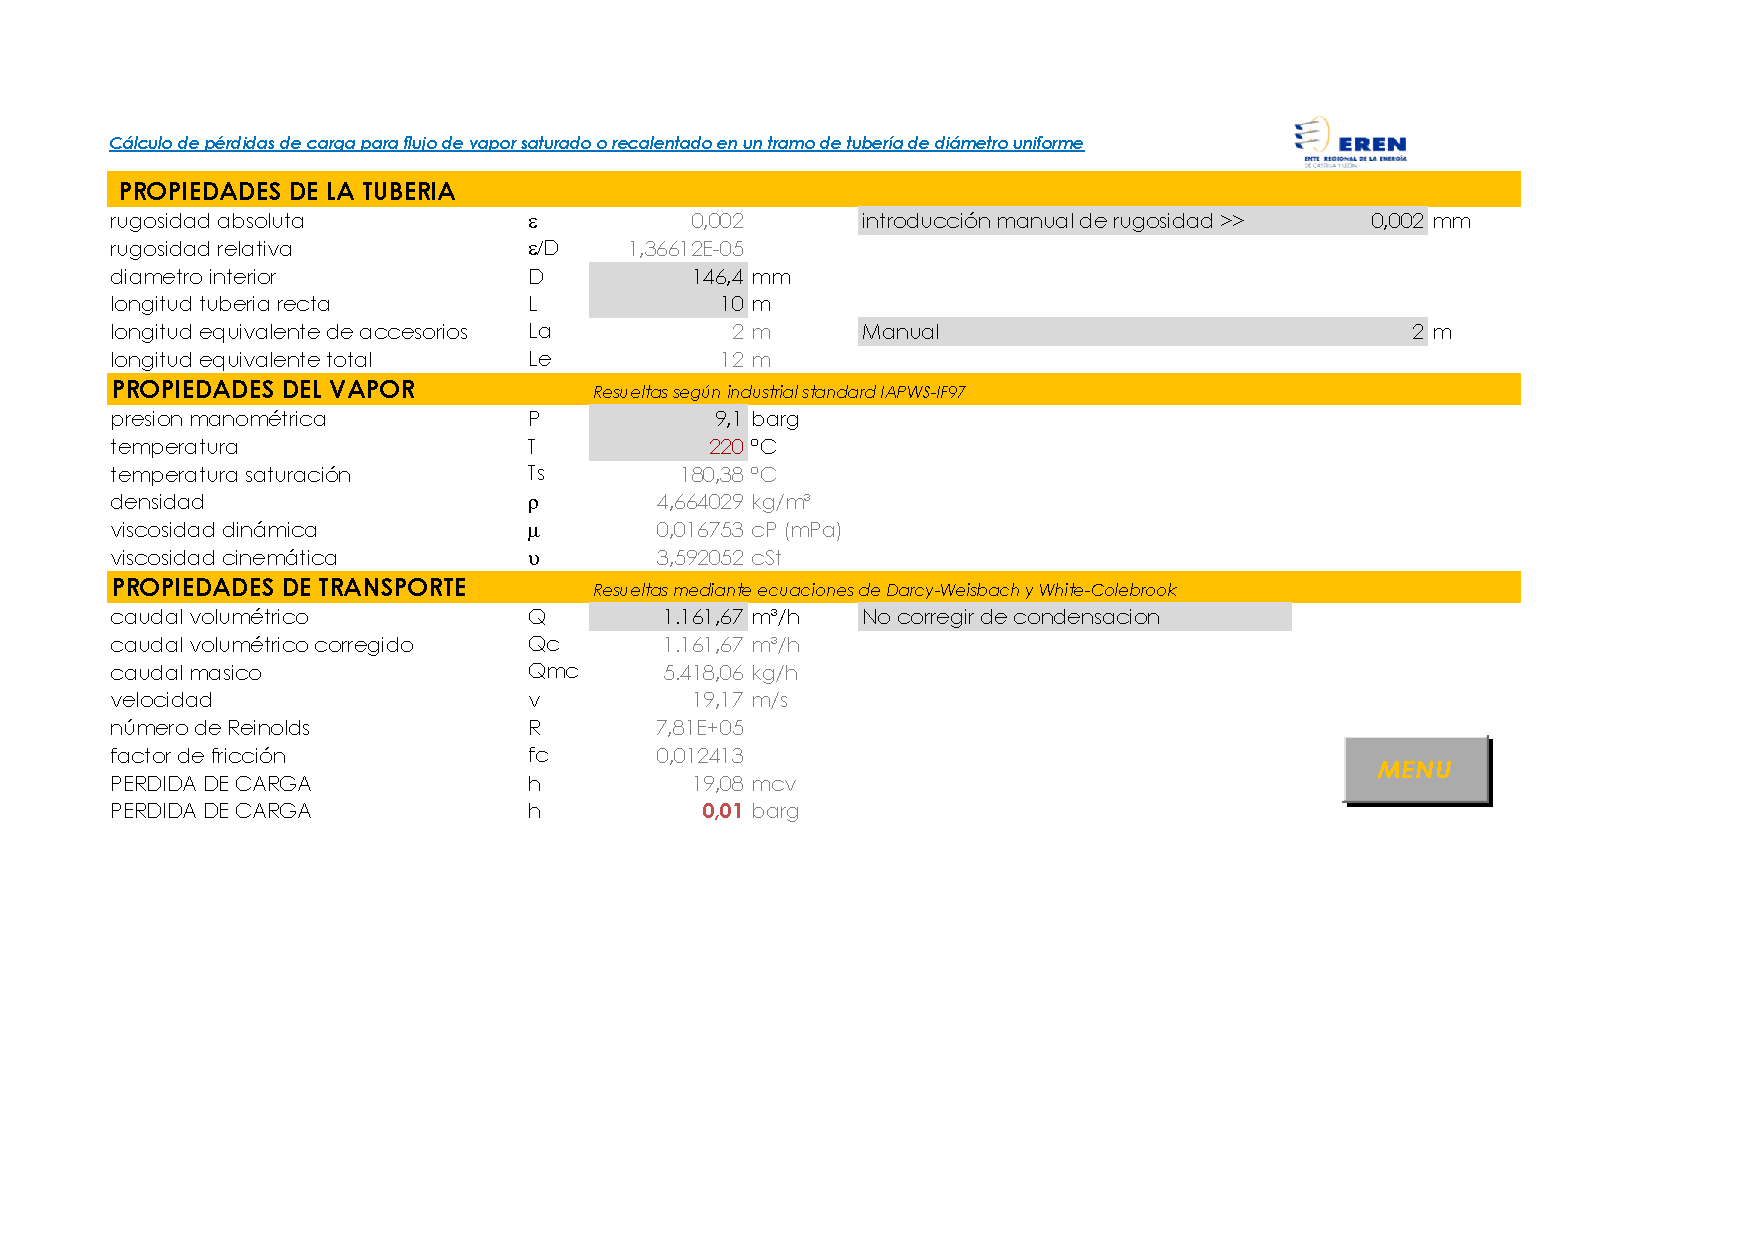
\includegraphics[trim={1cm 6cm 4cm 2cm}, clip, width=\textwidth]{Figuras/calculos_tramos/Vapor_TR1_Caldera-P.pdf}
	\caption{Hoja de cálculo del Tramo 1 (Caldera-P)}
	\label{fig:hoja-calculo-tramo1}
\end{figure}

El croquis del tramo con su trazado y puntos característicos se presenta en la \figref{fig:croquis-tramo1}.

\begin{figure}[H]
	\centering
	
\includegraphics[width=0.75\textwidth]{Figuras/dibujos_tramos/Vapor_TR1_Caldera-P.pdf}
	\caption{Croquis del Tramo 1 (Caldera-P)}
	\label{fig:croquis-tramo1}
\end{figure}

% =================================================================
% Sección 2.2.4: Tramo 2 (P-C1) - Tramo enterrado
% Generado por latex-writer | Fecha: 2026-03-25
% =================================================================

\subsubsection{Tramo 2: P-C$_1$ (tramo enterrado)}
\label{subsubsec:tramo2-p-c1}

Este tramo conecta el punto de derivación P con el consumidor C$_1$, constituyendo el tramo más largo de la instalación y el único con disposición enterrada. Esta configuración impone requisitos específicos tanto en la selección del material como en las condiciones de instalación.

\paragraph{Datos de partida}

Los datos geométricos y de servicio del tramo se recogen en la \tabref{tab:datos-tramo2}.

\begin{table}[H]
	\centering
	\caption{Datos de partida del Tramo 2 (P-C$_1$)}
	\label{tab:datos-tramo2}
	\begin{tabular}{lcc}
		\toprule
		\textbf{Parámetro}                & \textbf{Valor}                                     & \textbf{Unidad} \\
		\midrule
		Longitud real                     & 88{,}189                                           & m               \\
		Longitud equivalente (accesorios) & 9{,}24                                             & m               \\
		Longitud de cálculo               & 97{,}429                                           & m               \\
		Caudal másico                     & 679                                                & kg/h            \\
		Accesorios                        & \multicolumn{2}{c}{2 codos 90° + 1 T (paso recto)}                   \\
		\bottomrule
	\end{tabular}
\end{table}

\paragraph{Tubería seleccionada}

Dada la condición de tramo enterrado, se selecciona una tubería con pared muy reforzada para garantizar la resistencia mecánica frente a las cargas del terreno y proporcionar mayor protección contra la corrosión por contacto con el suelo. Las características de la tubería se muestran en la \tabref{tab:tuberia-tramo2}.

\begin{table}[H]
	\centering
	\caption{Tubería seleccionada para el Tramo 2}
	\label{tab:tuberia-tramo2}
	\begin{tabular}{lcc}
		\toprule
		\textbf{Parámetro} & \textbf{Valor}                   & \textbf{Unidad} \\
		\midrule
		Norma              & \multicolumn{2}{c}{Schedule 160}                   \\
		Diámetro nominal   & DN~80                            & ---             \\
		Diámetro interior  & 66{,}6                           & mm              \\
		Diámetro exterior  & 88{,}9                           & mm              \\
		\bottomrule
	\end{tabular}
\end{table}

La selección de Schedule 160 frente a alternativas de menor espesor (Schedule 40 o 80) se justifica por:
\begin{itemize}[noitemsep]
	\item Resistencia mecánica ante cargas verticales del terreno y posibles sobrecargas superficiales.
	\item Mayor margen de seguridad frente a corrosión exterior por contacto con el suelo.
	\item Compensación de posibles defectos de instalación en tramos de difícil inspección.
\end{itemize}

\paragraph{Verificación hidráulica}

Los resultados de la verificación hidráulica se presentan en la \tabref{tab:hidraulica-tramo2}. Este tramo presenta la mayor pérdida de carga de toda la red de vapor debido a su longitud.

\begin{table}[H]
	\centering
	\caption{Verificación hidráulica del Tramo 2}
	\label{tab:hidraulica-tramo2}
	\begin{tabular}{lcc}
		\toprule
		\textbf{Parámetro} & \textbf{Valor} & \textbf{Unidad} \\
		\midrule
		Velocidad real     & 18{,}93        & m/s             \\
		Pérdida de carga   & 0{,}24         & bar             \\
		Presión de entrada & 9{,}058        & bar(g)          \\
		Presión de salida  & 8{,}818        & bar(g)          \\
		\bottomrule
	\end{tabular}
\end{table}

La velocidad de 18{,}93~m/s se encuentra dentro del rango admisible (15--30~m/s). La pérdida de carga de 0{,}24~bar representa el valor máximo de la red, lo cual resulta coherente con la mayor longitud de este tramo.

\paragraph{Condiciones de enterramiento}

Las condiciones de instalación del tramo enterrado se resumen en la \tabref{tab:enterramiento-tramo2}. El análisis térmico detallado de las pérdidas de calor al terreno se desarrolla en la Sección 2.4 dedicada al aislamiento térmico.

\begin{table}[H]
	\centering
	\caption{Condiciones de enterramiento del Tramo 2}
	\label{tab:enterramiento-tramo2}
	\begin{tabular}{lcc}
		\toprule
		\textbf{Parámetro}             & \textbf{Valor}                          & \textbf{Unidad} \\
		\midrule
		Profundidad del eje de tubería & 1{,}09                                  & m               \\
		Profundidad total de zanja     & 1{,}34                                  & m               \\
		Ancho de zanja                 & 1{,}50                                  & m               \\
		Aislamiento térmico            & \multicolumn{2}{c}{Lana de Roca, 50~mm}                   \\
		Protección mecánica            & \multicolumn{2}{c}{Losa HA-25, 10~cm}                     \\
		\bottomrule
	\end{tabular}
\end{table}

\paragraph{Presión en el consumidor C$_1$}

El consumidor C$_1$ requiere una presión de trabajo de 4~bar(g) con un caudal de 679~kg/h. La presión disponible a la salida del tramo es de 8{,}818~bar(g), lo que proporciona un margen de +4{,}818~bar respecto a la presión requerida. Este exceso de presión se regulará mediante una válvula reductora de presión instalada en la acometida al consumidor.

\paragraph{Resultados}

En la \tabref{tab:resumen-tramo2} se presenta el resumen de resultados del dimensionado del Tramo 2.

\begin{table}[H]
	\centering
	\caption{Resumen de resultados del Tramo 2 (P-C$_1$)}
	\label{tab:resumen-tramo2}
	\begin{tabular}{lcc}
		\toprule
		\textbf{Parámetro}        & \textbf{Valor}                            & \textbf{Unidad} \\
		\midrule
		Tubería                   & \multicolumn{2}{c}{Schedule 160 -- DN~80}                   \\
		Diámetro interior         & 66{,}6                                    & mm              \\
		Longitud total de cálculo & 97{,}429                                  & m               \\
		Caudal másico             & 679                                       & kg/h            \\
		Velocidad                 & 18{,}93                                   & m/s             \\
		Pérdida de carga          & 0{,}24                                    & bar             \\
		Presión entrada           & 9{,}058                                   & bar(g)          \\
		Presión salida (C$_1$)    & 8{,}818                                   & bar(g)          \\
		\bottomrule
	\end{tabular}
\end{table}

Los cálculos detallados de pérdida de carga se muestran en la \figref{fig:calculos-tramo2}, mientras que el esquema del tramo con sus cotas y accesorios se presenta en la \figref{fig:dibujo-tramo2}.

\begin{figure}[H]
	\centering
	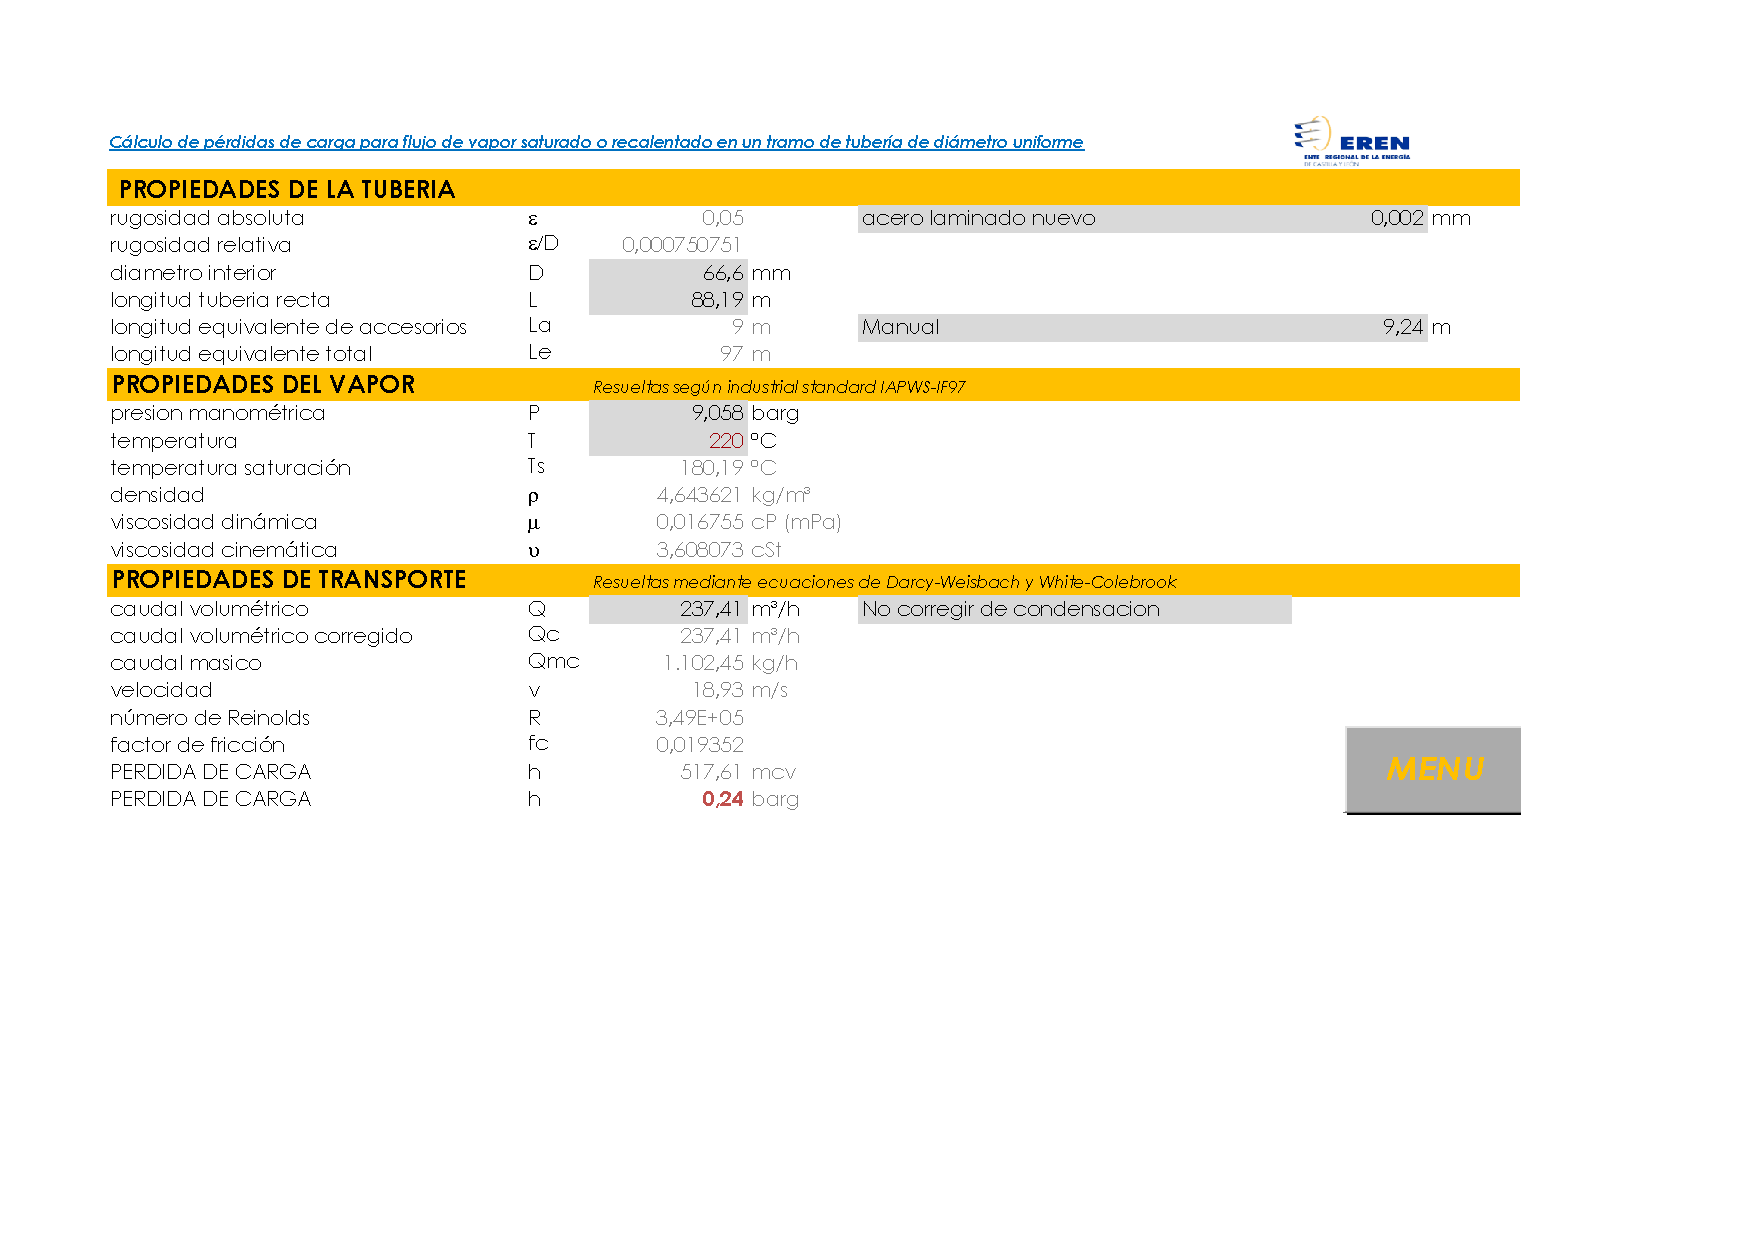
\includegraphics[width=\textwidth]{Figuras/calculos_tramos/Vapor_TR2_P-C1.pdf}
	\caption{Cálculos de pérdida de carga para el Tramo 2 (P-C$_1$)}
	\label{fig:calculos-tramo2}
\end{figure}

\begin{figure}[H]
	\centering
	
\includegraphics[width=\textwidth]{Figuras/dibujos_tramos/Vapor_TR2_P-C1.pdf}
	\caption{Esquema del Tramo 2 (P-C$_1$) con disposición enterrada}
	\label{fig:dibujo-tramo2}
\end{figure}

% =================================================================
% Sección 2.2.5: Tramo 3 (P-S)
% Generado por latex-writer | Fecha: 2026-03-25
% =================================================================

\subsubsection{Tramo 3: P-S}
\label{subsubsec:tramo3-p-s}

El tramo P-S constituye la línea principal que alimenta a los consumidores C$_2$, C$_3$ y C$_4$, transportando el caudal combinado de estos tres puntos de consumo.

\paragraph{Datos de partida}

Los datos geométricos y de servicio del tramo se presentan en la \tabref{tab:datos-tramo3}.

\begin{table}[H]
	\centering
	\caption{Datos de partida del Tramo 3 (P-S)}
	\label{tab:datos-tramo3}
	\begin{tabular}{lcc}
		\toprule
		\textbf{Parámetro}   & \textbf{Valor}                                    & \textbf{Unidad} \\
		\midrule
		Longitud real        & 106                                               & m               \\
		Longitud equivalente & 25{,}44                                           & m               \\
		Longitud de cálculo  & 131{,}44                                          & m               \\
		Caudal másico        & 3737                                              & kg/h            \\
		Accesorios           & \multicolumn{2}{c}{1 codo 90° + 2 T (derivación)}                   \\
		\bottomrule
	\end{tabular}
\end{table}

El caudal másico corresponde a la suma de los consumidores alimentados: $\dot{m} = C_2 + C_3 + C_4 = 1359 + 340 + 2038 = 3737$~kg/h.

\paragraph{Tubería seleccionada}

\begin{table}[H]
	\centering
	\caption{Tubería seleccionada para el Tramo 3}
	\label{tab:tuberia-tramo3}
	\begin{tabular}{lcc}
		\toprule
		\textbf{Parámetro} & \textbf{Valor}               & \textbf{Unidad} \\
		\midrule
		Norma              & \multicolumn{2}{c}{DIN 2448}                   \\
		Diámetro nominal   & DN~125                       & ---             \\
		Diámetro interior  & 131{,}7                      & mm              \\
		\bottomrule
	\end{tabular}
\end{table}

\paragraph{Verificación hidráulica}

\begin{table}[H]
	\centering
	\caption{Verificación hidráulica del Tramo 3}
	\label{tab:hidraulica-tramo3}
	\begin{tabular}{lcc}
		\toprule
		\textbf{Parámetro} & \textbf{Valor} & \textbf{Unidad} \\
		\midrule
		Velocidad real     & 20{,}28        & m/s             \\
		Pérdida de carga   & 0{,}16         & bar             \\
		Presión de entrada & 9{,}058        & bar(g)          \\
		Presión de salida  & 8{,}90         & bar(g)          \\
		\bottomrule
	\end{tabular}
\end{table}

La velocidad de 20{,}28~m/s está dentro del rango objetivo de diseño. Los cálculos detallados se muestran en la \figref{fig:calculos-tramo3}.

\begin{figure}[H]
	\centering
	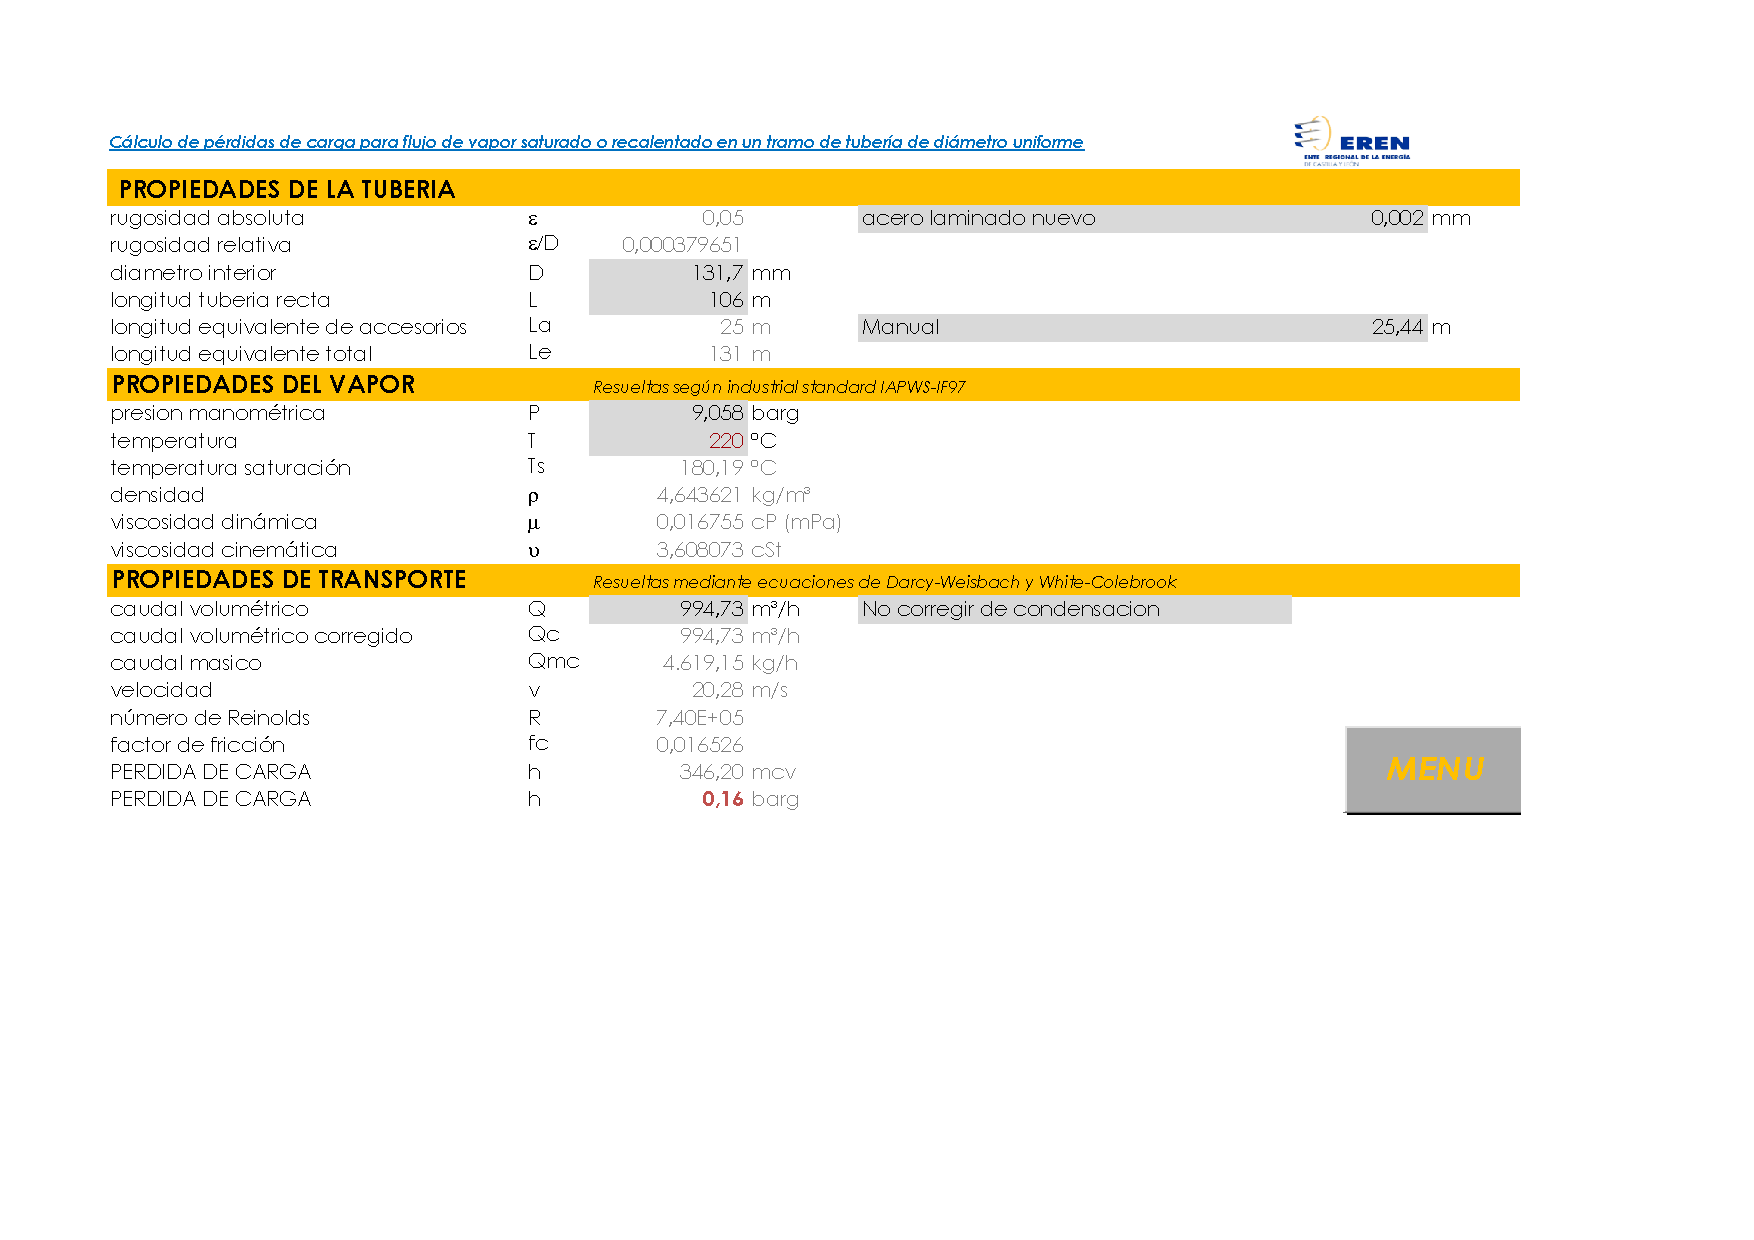
\includegraphics[width=\textwidth]{Figuras/calculos_tramos/Vapor_TR3_P-S.pdf}
	\caption{Hoja de cálculo del Tramo 3 (P-S)}
	\label{fig:calculos-tramo3}
\end{figure}

% =================================================================
% Sección 2.2.6: Tramo 4 (S-C2)
% Generado por latex-writer | Fecha: 2026-03-25
% =================================================================

\subsubsection{Tramo 4: S-C$_2$}
\label{subsubsec:tramo4-s-c2}

Este tramo conecta el nodo S con el consumidor C$_2$, siendo un tramo relativamente corto y sin accesorios significativos.

\paragraph{Datos de partida}

\begin{table}[H]
	\centering
	\caption{Datos de partida del Tramo 4 (S-C$_2$)}
	\label{tab:datos-tramo4}
	\begin{tabular}{lcc}
		\toprule
		\textbf{Parámetro}   & \textbf{Valor}                            & \textbf{Unidad} \\
		\midrule
		Longitud real        & 25                                        & m               \\
		Longitud equivalente & 5                                         & m               \\
		Longitud de cálculo  & 30                                        & m               \\
		Caudal másico        & 1359                                      & kg/h            \\
		Accesorios           & \multicolumn{2}{c}{Ninguno (tramo recto)}                   \\
		\bottomrule
	\end{tabular}
\end{table}

La longitud equivalente se estima como el 20\% de la longitud real al no presentar accesorios significativos.

\paragraph{Tubería seleccionada}

\begin{table}[H]
	\centering
	\caption{Tubería seleccionada para el Tramo 4}
	\label{tab:tuberia-tramo4}
	\begin{tabular}{lcc}
		\toprule
		\textbf{Parámetro} & \textbf{Valor}               & \textbf{Unidad} \\
		\midrule
		Norma              & \multicolumn{2}{c}{DIN 2448}                   \\
		Diámetro nominal   & DN~80                        & ---             \\
		Diámetro interior  & 82{,}5                       & mm              \\
		\bottomrule
	\end{tabular}
\end{table}

\paragraph{Verificación hidráulica}

\begin{table}[H]
	\centering
	\caption{Verificación hidráulica del Tramo 4}
	\label{tab:hidraulica-tramo4}
	\begin{tabular}{lcc}
		\toprule
		\textbf{Parámetro} & \textbf{Valor} & \textbf{Unidad} \\
		\midrule
		Velocidad real     & 21{,}45        & m/s             \\
		Pérdida de carga   & 0{,}07         & bar             \\
		Presión de entrada & 8{,}90         & bar(g)          \\
		Presión de salida  & 8{,}83         & bar(g)          \\
		\bottomrule
	\end{tabular}
\end{table}

La presión de salida de 8{,}83~bar(g) supera ampliamente la presión requerida por C$_2$ (7~bar(g)), proporcionando un margen de 1{,}83~bar. Los cálculos detallados se muestran en la \figref{fig:calculos-tramo4}.

\begin{figure}[H]
	\centering
	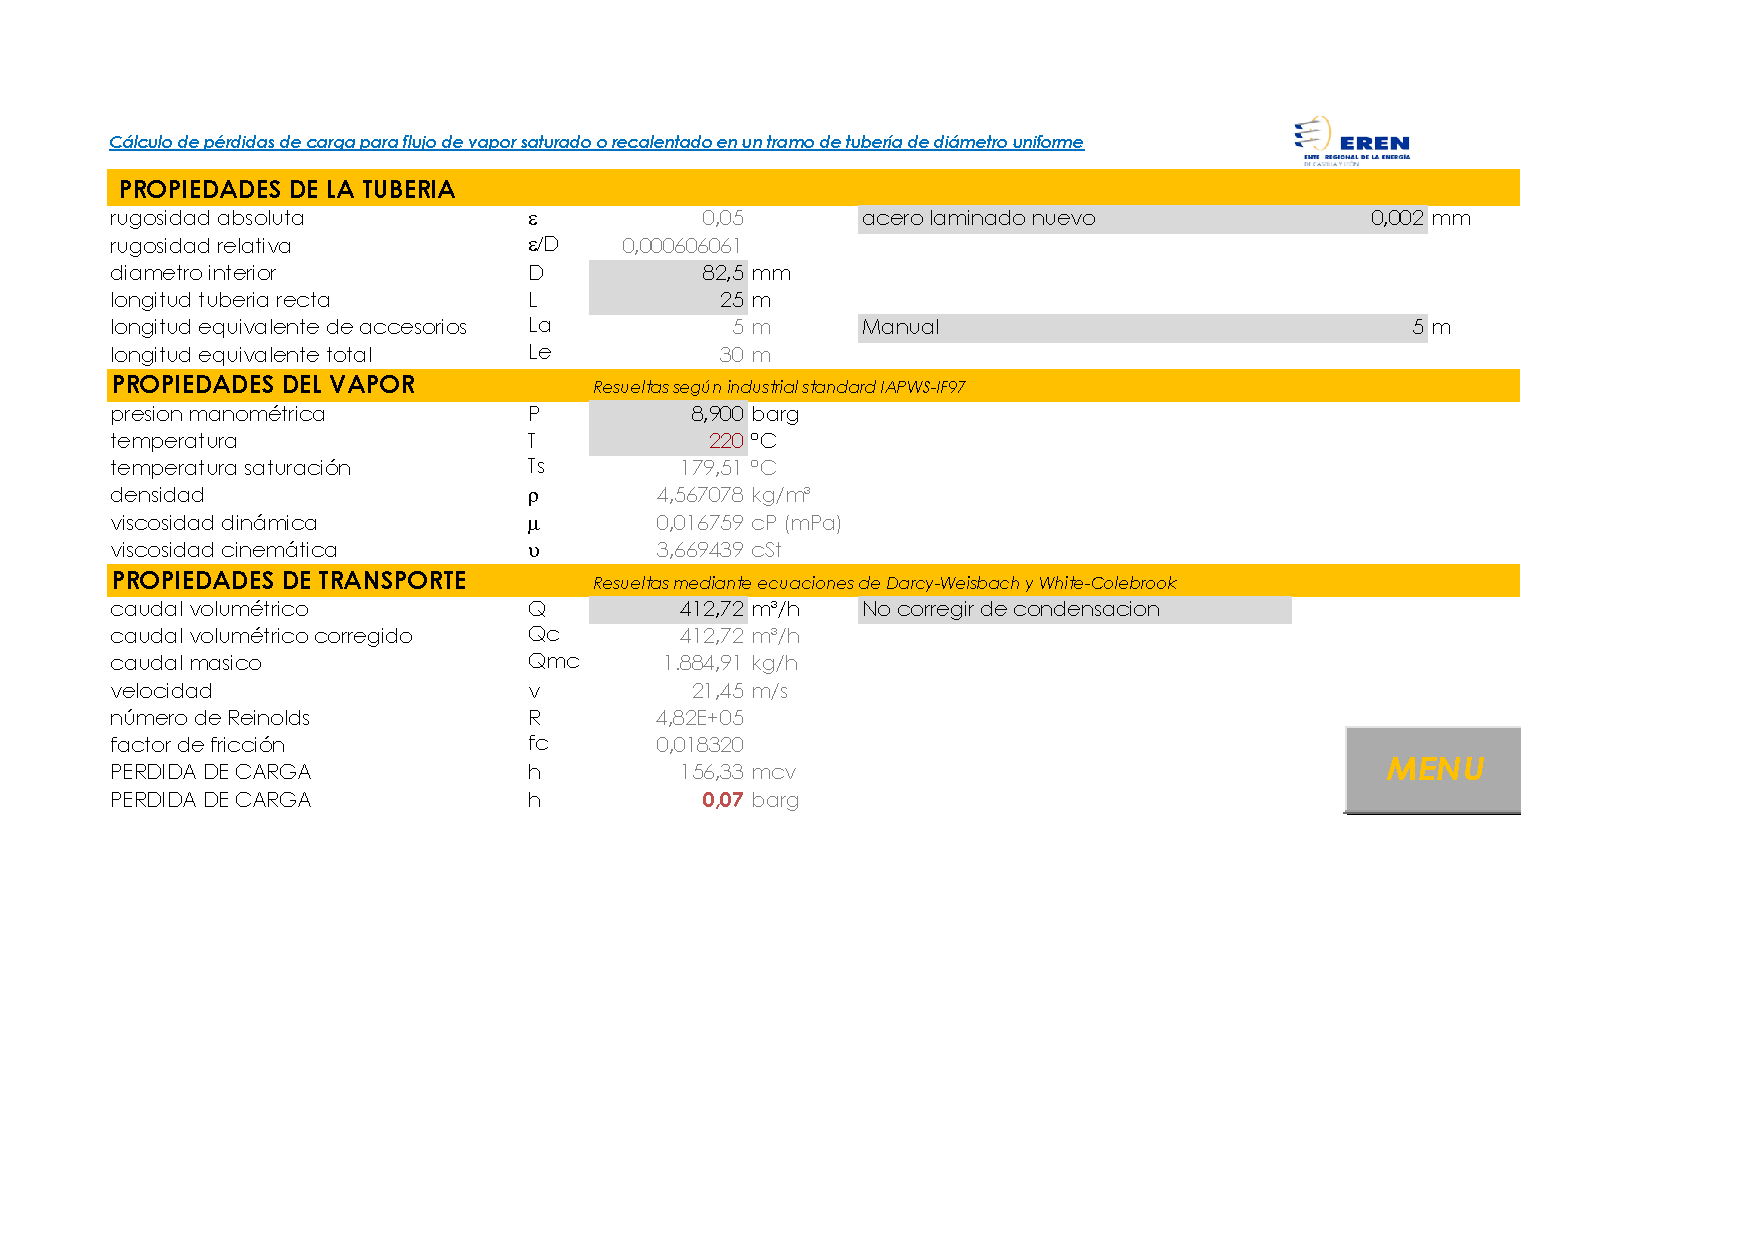
\includegraphics[width=\textwidth]{Figuras/calculos_tramos/Vapor_TR4_S-C2.pdf}
	\caption{Hoja de cálculo del Tramo 4 (S-C$_2$)}
	\label{fig:calculos-tramo4}
\end{figure}

% =================================================================
% Sección 2.2.7: Tramos 5, 6 y 7 (S-T, T-C3, T-C4)
% Generado por latex-writer | Fecha: 2026-03-25
% =================================================================

\subsubsection{Tramos 5, 6 y 7: rama S-T-C$_3$-C$_4$}
\label{subsubsec:tramos5-6-7}

Los tramos 5, 6 y 7 conforman la rama que alimenta a los consumidores C$_3$ y C$_4$, partiendo del nodo S. El nodo T actúa como punto de bifurcación hacia estos dos consumidores.

\paragraph{Tramo 5: S-T}

El tramo S-T transporta el caudal combinado de C$_3$ y C$_4$.

\begin{table}[H]
	\centering
	\caption{Datos y resultados del Tramo 5 (S-T)}
	\label{tab:tramo5}
	\begin{tabular}{lcc}
		\toprule
		\textbf{Parámetro}   & \textbf{Valor}                                     & \textbf{Unidad} \\
		\midrule
		Longitud real        & 60                                                 & m               \\
		Longitud equivalente & 7{,}5                                              & m               \\
		Longitud de cálculo  & 78                                                 & m               \\
		Caudal másico        & 2378                                               & kg/h            \\
		Accesorios           & \multicolumn{2}{c}{1 T (recta) + 1 T (derivación)}                   \\
		Tubería              & \multicolumn{2}{c}{DIN 2448 -- DN~100}                               \\
		Diámetro interior    & 107{,}1                                            & mm              \\
		Velocidad            & 20{,}79                                            & m/s             \\
		Pérdida de carga     & 0{,}12                                             & bar             \\
		Presión entrada      & 8{,}90                                             & bar(g)          \\
		Presión salida       & 8{,}78                                             & bar(g)          \\
		\bottomrule
	\end{tabular}
\end{table}

\paragraph{Tramo 6: T-C$_3$}

Este tramo alimenta al consumidor C$_3$, siendo el de menor caudal de la instalación.

\begin{table}[H]
	\centering
	\caption{Datos y resultados del Tramo 6 (T-C$_3$)}
	\label{tab:tramo6}
	\begin{tabular}{lcc}
		\toprule
		\textbf{Parámetro}   & \textbf{Valor}                            & \textbf{Unidad} \\
		\midrule
		Longitud real        & 15                                        & m               \\
		Longitud equivalente & 3                                         & m               \\
		Longitud de cálculo  & 18                                        & m               \\
		Caudal másico        & 340                                       & kg/h            \\
		Accesorios           & \multicolumn{2}{c}{Ninguno (tramo corto)}                   \\
		Tubería              & \multicolumn{2}{c}{Schedule 40 -- DN~50}                    \\
		Diámetro interior    & 52{,}5                                    & mm              \\
		Velocidad            & 20{,}42                                   & m/s             \\
		Pérdida de carga     & 0{,}07                                    & bar             \\
		Presión entrada      & 8{,}78                                    & bar(g)          \\
		Presión salida       & 8{,}71                                    & bar(g)          \\
		\bottomrule
	\end{tabular}
\end{table}

\paragraph{Tramo 7: T-C$_4$}

El tramo T-C$_4$ alimenta al consumidor de mayor caudal de la instalación.

\begin{table}[H]
	\centering
	\caption{Datos y resultados del Tramo 7 (T-C$_4$)}
	\label{tab:tramo7}
	\begin{tabular}{lcc}
		\toprule
		\textbf{Parámetro}   & \textbf{Valor}                                & \textbf{Unidad} \\
		\midrule
		Longitud real        & 45                                            & m               \\
		Longitud equivalente & 12{,}4                                        & m               \\
		Longitud de cálculo  & 57{,}4                                        & m               \\
		Caudal másico        & 2038                                          & kg/h            \\
		Accesorios           & \multicolumn{2}{c}{2 codos 90° + 1 T (recta)}                   \\
		Tubería              & \multicolumn{2}{c}{Schedule 40 -- DN~100}                       \\
		Diámetro interior    & 102{,}3                                       & mm              \\
		Velocidad            & 20{,}11                                       & m/s             \\
		Pérdida de carga     & 0{,}09                                        & bar             \\
		Presión entrada      & 8{,}78                                        & bar(g)          \\
		Presión salida       & 8{,}69                                        & bar(g)          \\
		\bottomrule
	\end{tabular}
\end{table}

Los tres tramos mantienen velocidades muy próximas al objetivo de diseño (20~m/s), confirmando la coherencia del dimensionado. Las hojas de cálculo detalladas se presentan en las Figuras \ref{fig:calculos-tramo5}, \ref{fig:calculos-tramo6} y \ref{fig:calculos-tramo7}.

\begin{figure}[H]
	\centering
	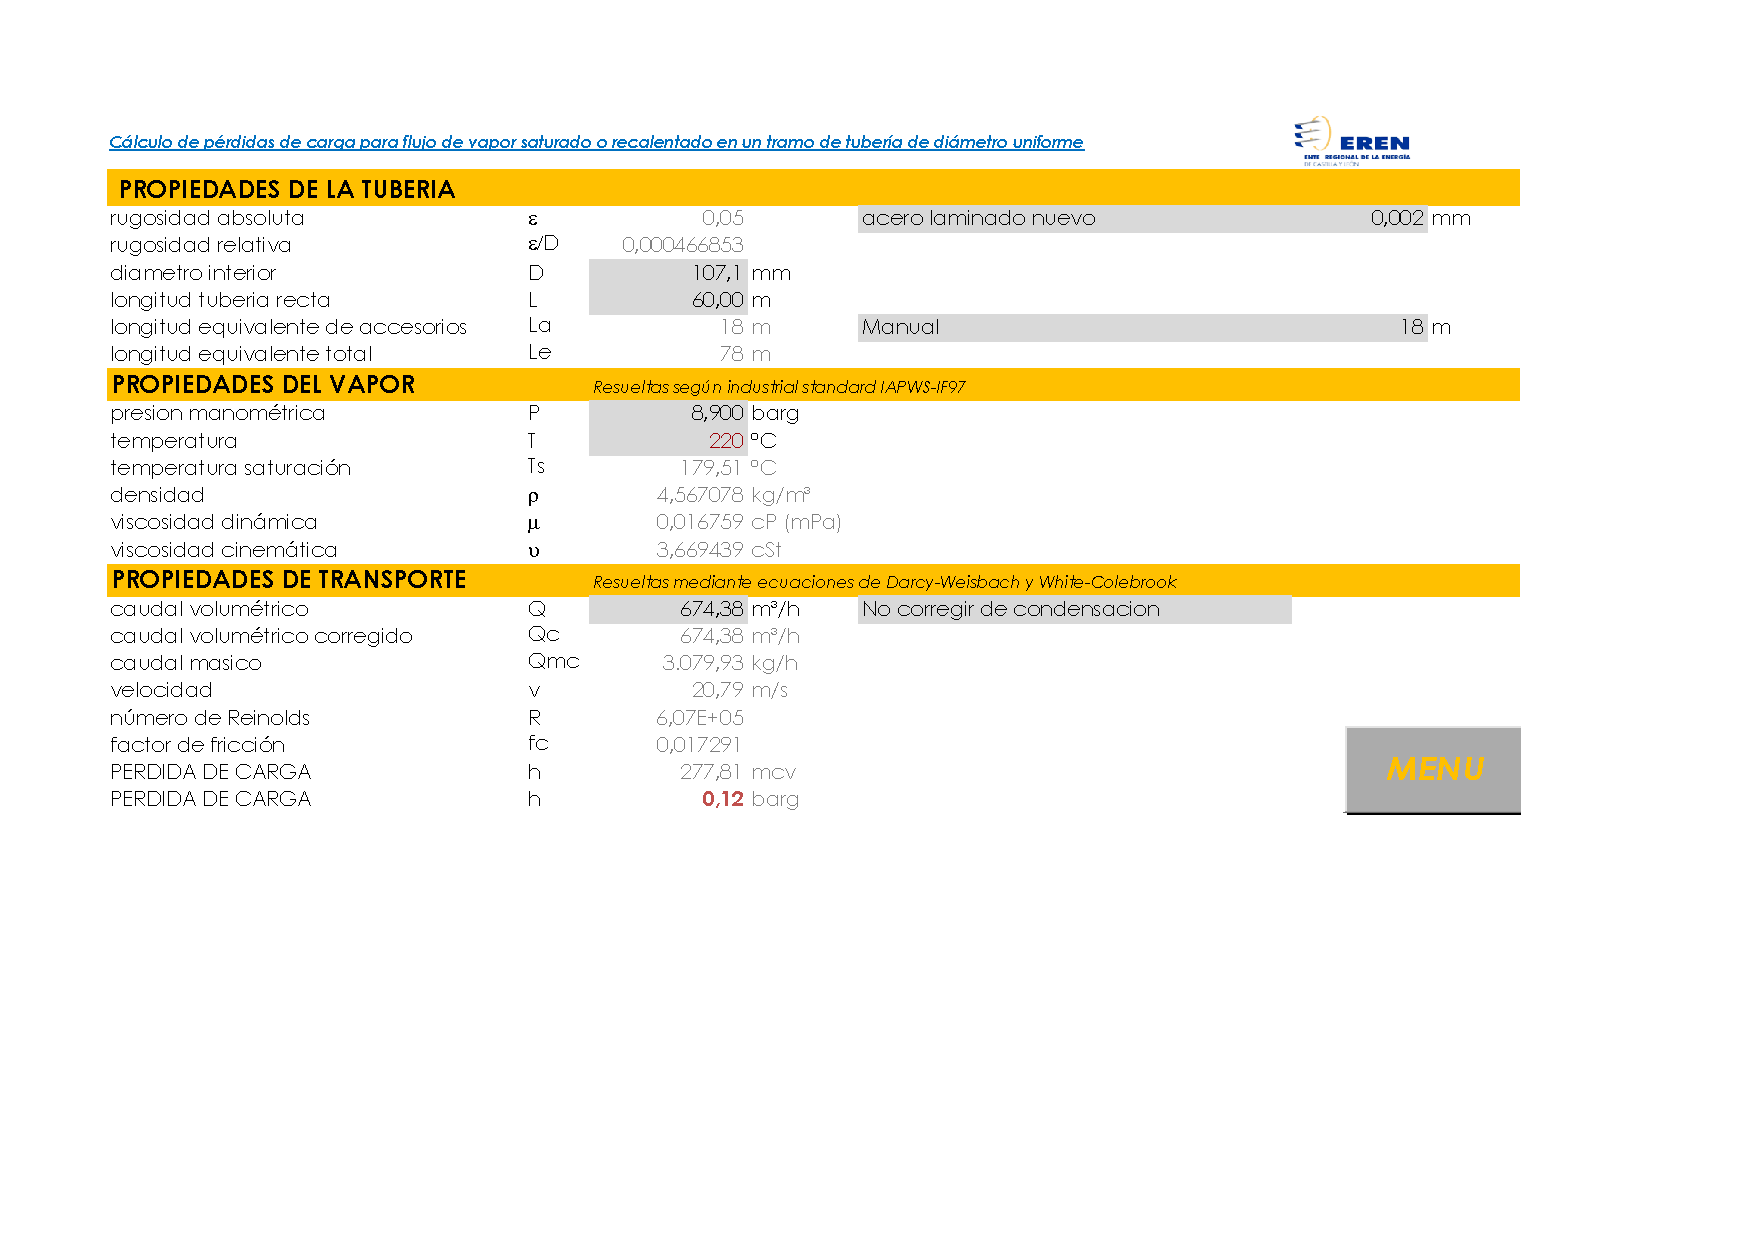
\includegraphics[width=\textwidth]{Figuras/calculos_tramos/Vapor_TR5_S-T.pdf}
	\caption{Hoja de cálculo del Tramo 5 (S-T)}
	\label{fig:calculos-tramo5}
\end{figure}

\begin{figure}[H]
	\centering
	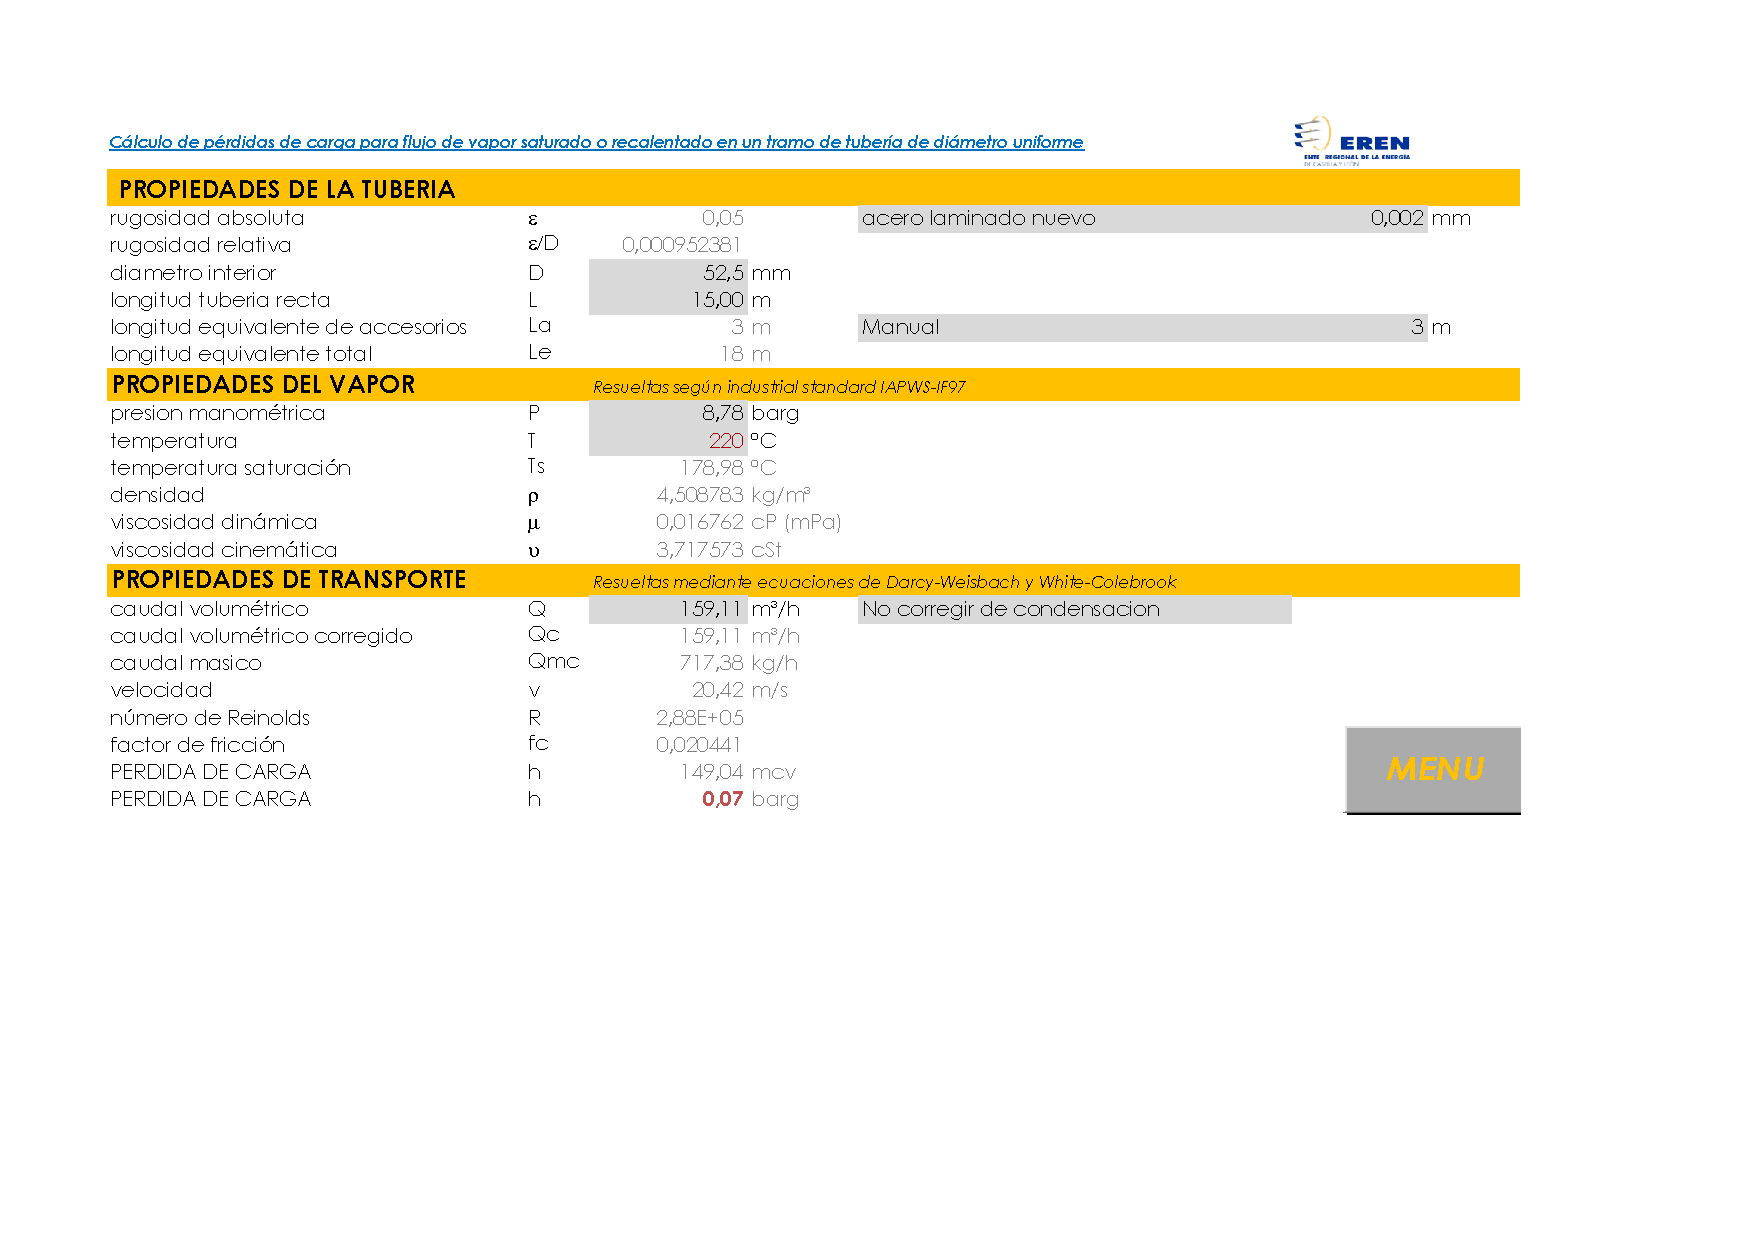
\includegraphics[width=\textwidth]{Figuras/calculos_tramos/Vapor_TR6_T-C3.pdf}
	\caption{Hoja de cálculo del Tramo 6 (T-C$_3$)}
	\label{fig:calculos-tramo6}
\end{figure}

\begin{figure}[H]
	\centering
	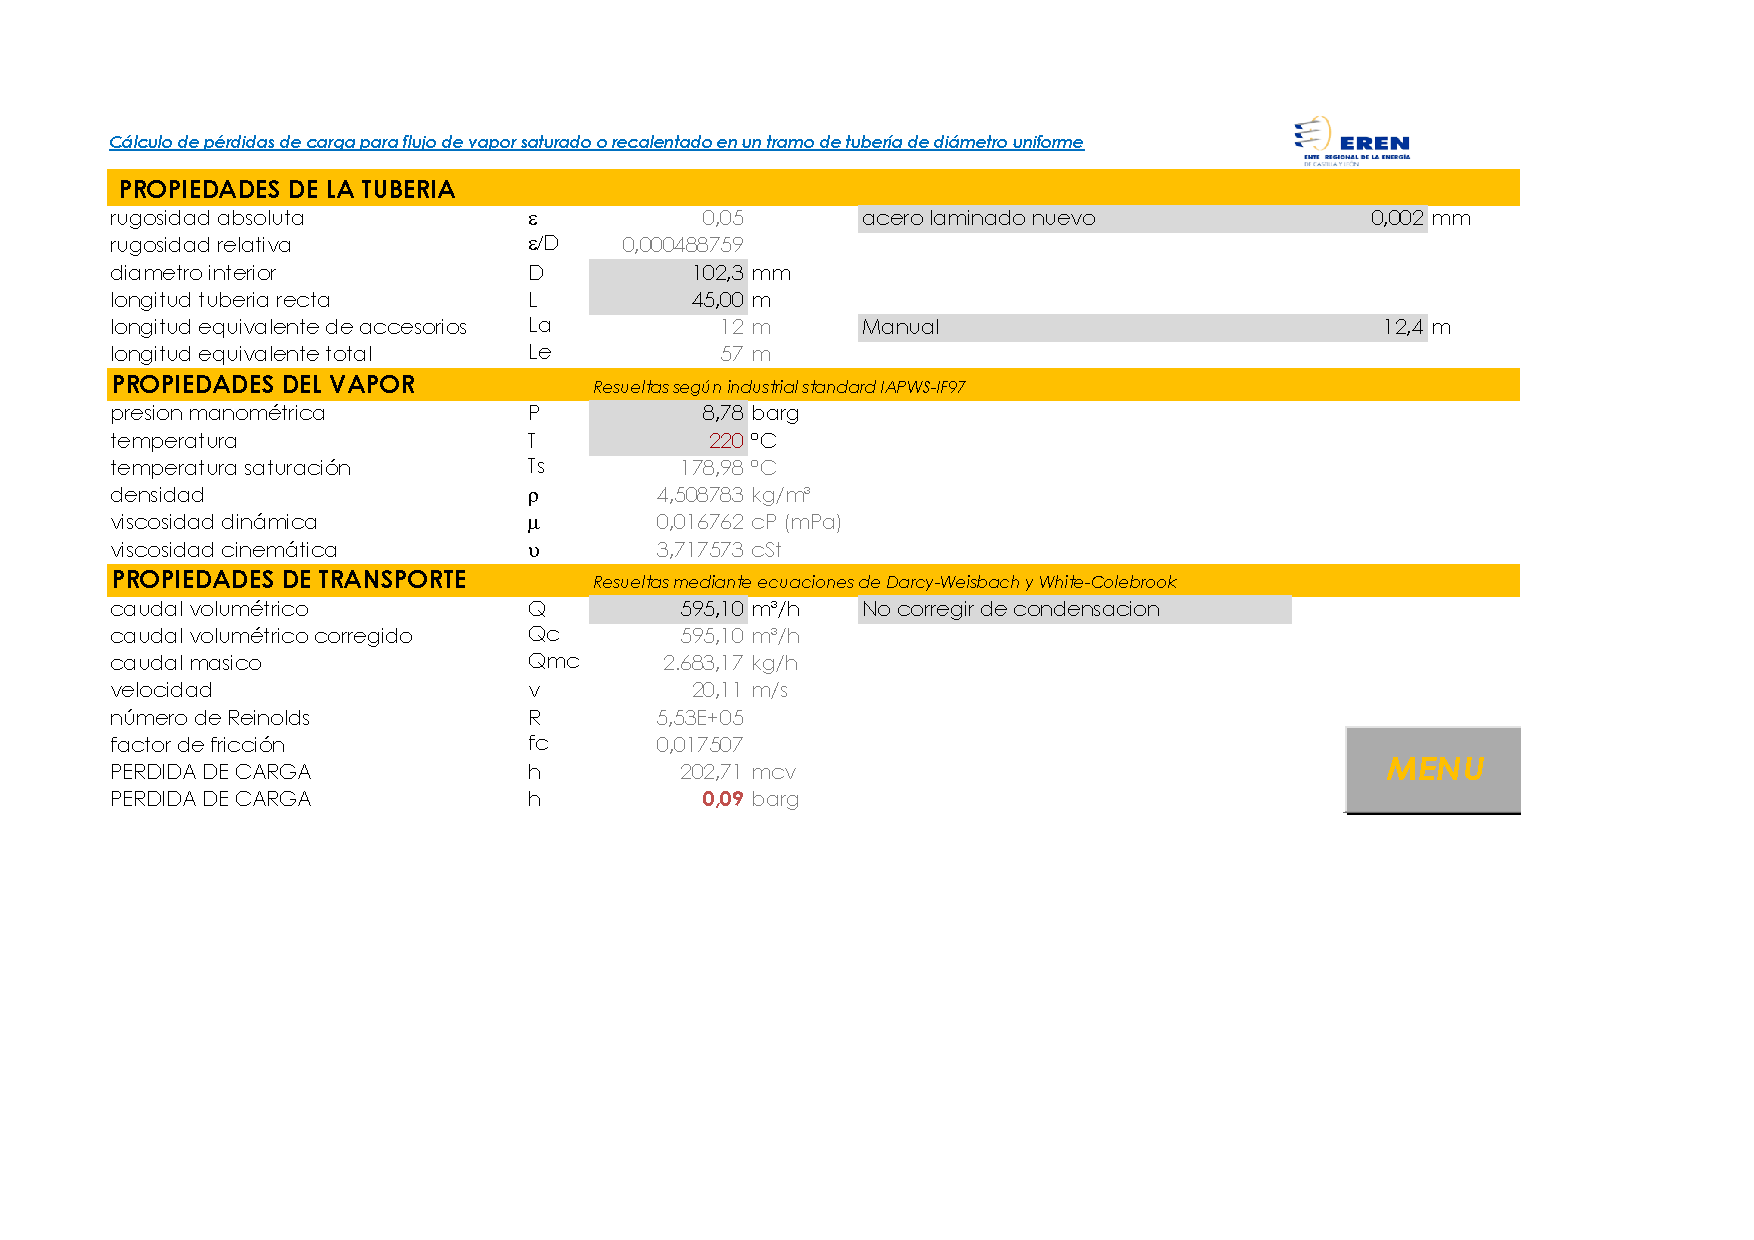
\includegraphics[width=\textwidth]{Figuras/calculos_tramos/Vapor_TR7_T-C4.pdf}
	\caption{Hoja de cálculo del Tramo 7 (T-C$_4$)}
	\label{fig:calculos-tramo7}
\end{figure}

% =================================================================
% Sección 2.2.8: Resumen de la red de vapor
% Generado por latex-writer | Fecha: 2026-03-25
% =================================================================

\subsubsection{Resumen de la red de vapor}
\label{subsubsec:resumen-red-vapor}

En la \tabref{tab:resumen-red-vapor} se presenta el resumen completo de los resultados del dimensionado hidráulico de la red de vapor.

\begin{table}[H]
	\centering
	\caption{Resumen de diámetros, velocidades y pérdidas de carga de la red de vapor}
	\label{tab:resumen-red-vapor}
	\begin{tabular}{lcccccc}
		\toprule
		\textbf{Tramo} & \textbf{Tubería} & \textbf{$D_{int}$} & \textbf{$L_{cálc}$} & \textbf{$\dot{m}$} & \textbf{$v$} & \textbf{$\Delta P$} \\
		               &                  & (mm)               & (m)                 & (kg/h)             & (m/s)        & (bar)               \\
		\midrule
		1: Caldera-P   & Sch.80 DN~150    & 146{,}4            & 15{,}29             & 5400               & 19{,}17      & 0{,}01              \\
		2: P-C$_1$     & Sch.160 DN~80    & 66{,}6             & 97{,}43             & 679                & 18{,}93      & 0{,}24              \\
		3: P-S         & DIN DN~125       & 131{,}7            & 131{,}44            & 3737               & 20{,}28      & 0{,}16              \\
		4: S-C$_2$     & DIN DN~80        & 82{,}5             & 30                  & 1359               & 21{,}45      & 0{,}07              \\
		5: S-T         & DIN DN~100       & 107{,}1            & 78                  & 2378               & 20{,}79      & 0{,}12              \\
		6: T-C$_3$     & Sch.40 DN~50     & 52{,}5             & 18                  & 340                & 20{,}42      & 0{,}07              \\
		7: T-C$_4$     & Sch.40 DN~100    & 102{,}3            & 57{,}4              & 2038               & 20{,}11      & 0{,}09              \\
		\bottomrule
	\end{tabular}
\end{table}

\paragraph{Verificación de presiones en consumidores}

La \tabref{tab:presiones-consumidores} muestra las presiones disponibles en cada punto de consumo y su comparación con los requisitos.

\begin{table}[H]
	\centering
	\caption{Presiones disponibles vs. requeridas en los consumidores}
	\label{tab:presiones-consumidores}
	\begin{tabular}{lcccc}
		\toprule
		\textbf{Consumidor} & \textbf{$P_{disponible}$} & \textbf{$P_{requerida}$} & \textbf{Margen} & \textbf{Estado} \\
		                    & bar(g)                    & bar(g)                   & bar             &                 \\
		\midrule
		C$_1$               & 8{,}818                   & 4                        & +4{,}818        & \checkmark      \\
		C$_2$               & 8{,}83                    & 7                        & +1{,}83         & \checkmark      \\
		C$_3$               & 8{,}71                    & 7                        & +1{,}71         & \checkmark      \\
		C$_4$               & 8{,}69                    & 7                        & +1{,}69         & \checkmark      \\
		\bottomrule
	\end{tabular}
\end{table}

\paragraph{Pérdida de carga total por recorrido}

La pérdida de carga acumulada desde la caldera hasta cada consumidor se presenta en la \tabref{tab:perdidas-acumuladas}.

\begin{table}[H]
	\centering
	\caption{Pérdida de carga acumulada hasta cada consumidor}
	\label{tab:perdidas-acumuladas}
	\begin{tabular}{lcc}
		\toprule
		\textbf{Recorrido}          & \textbf{$\Delta P_{total}$}                  & \textbf{Criterio $<$ 1 bar} \\
		                            & (bar)                                        &                             \\
		\midrule
		Caldera $\rightarrow$ C$_1$ & $0{,}01 + 0{,}24 = 0{,}25$                   & \checkmark                  \\
		Caldera $\rightarrow$ C$_2$ & $0{,}01 + 0{,}16 + 0{,}07 = 0{,}24$          & \checkmark                  \\
		Caldera $\rightarrow$ C$_3$ & $0{,}01 + 0{,}16 + 0{,}12 + 0{,}07 = 0{,}36$ & \checkmark                  \\
		Caldera $\rightarrow$ C$_4$ & $0{,}01 + 0{,}16 + 0{,}12 + 0{,}09 = 0{,}38$ & \checkmark                  \\
		\bottomrule
	\end{tabular}
\end{table}

\paragraph{Conclusiones del dimensionado}

El dimensionado hidráulico de la red de vapor cumple satisfactoriamente con todos los criterios de diseño establecidos:

\begin{itemize}[noitemsep]
	\item Todas las velocidades se mantienen en el rango 18{,}93--21{,}45~m/s, próximas al objetivo de 20~m/s.
	\item Ningún tramo supera la velocidad máxima de 30~m/s.
	\item La pérdida de carga total máxima (0{,}38~bar hasta C$_4$) es inferior al criterio de 1~bar.
	\item Todos los consumidores disponen de presión suficiente con márgenes adecuados.
	\item El consumidor C$_1$ requiere válvula reductora debido a su menor presión de trabajo (4~bar(g)).
\end{itemize}

% =============================================================================
% Sección 2.3: Dimensionado Hidráulico de la Red de Condensados
% Generado por latex-writer | Fecha: 2026-03-25
% =============================================================================

\subsection{Dimensionado Hidráulico de la Red de Condensados}
\label{subsec:dimensionado-condensados}

La red de retorno de condensados constituye un elemento fundamental para la eficiencia energética de la instalación. El condensado generado en los consumidores retorna a la caldera mediante una red presurizada, aprovechando tanto la energía térmica residual del líquido como el vapor de revaporizado (vapor flash) generado en el proceso de expansión.

El diseño de esta red presenta particularidades respecto a la red de vapor, debido a la presencia de flujo bifásico (líquido + vapor flash) que requiere criterios de velocidad específicos y consideraciones adicionales de dimensionado.

\subsubsection{Consideraciones sobre Retorno de Condensados y Vapor Flash}
\label{subsubsec:consideraciones-condensados}

Cuando el condensado a alta presión (9~bar(g) en los consumidores) pasa a través del purgador y entra en la línea de retorno a menor presión, parte del condensado se revaporiza produciendo el denominado \textit{vapor flash} o \textit{vapor de revaporizado}. Este fenómeno se debe al exceso de entalpía del líquido respecto a las condiciones de saturación a la nueva presión.

\paragraph{Presión de diseño de la red de condensados}

La presión de diseño de la red de retorno se establece según el criterio:

\begin{equation}
	P_{red} = P_{min,consumidor} - 1~\text{bar} = 4 - 1 = 3~\text{bar(g)}
	\label{eq:presion-red-condensados}
\end{equation}

donde $P_{min,consumidor}$ corresponde a la presión mínima de trabajo entre todos los consumidores, en este caso el consumidor C$_1$ con 4~bar(g).

\paragraph{Características del flujo bifásico}

El vapor flash presenta un volumen específico significativamente mayor que el líquido, lo que determina las características del flujo en la tubería:

\begin{itemize}[noitemsep]
	\item Relación volumétrica aproximada: 98\% vapor, 2\% líquido
	\item Velocidad de diseño para flujo bifásico: 15--20~m/s (superior al condensado puro)
	\item El vapor flash representa energía recuperable aprovechable
\end{itemize}

\paragraph{Opciones de aprovechamiento del vapor flash}

El vapor de revaporizado puede aprovecharse mediante diferentes estrategias:

\begin{enumerate}[noitemsep]
	\item Tanques de revaporizado para separación de fases
	\item Inyección directa en procesos de baja presión
	\item Precalentamiento del agua de alimentación a la caldera
\end{enumerate}

\subsubsection{Cálculo del Porcentaje de Vapor Flash}
\label{subsubsec:calculo-vapor-flash}

El porcentaje de vapor flash generado se determina mediante un balance entálpico entre las condiciones de entrada (presión del consumidor) y las condiciones de la red de retorno.

\paragraph{Ecuación del balance entálpico}

\begin{equation}
	\%v_f = \frac{h_{l,P_1} - h_{l,P_2}}{h_{v,P_2} - h_{l,P_2}} \times 100
	\label{eq:vapor-flash}
\end{equation}

donde:
\begin{itemize}[noitemsep]
	\item $h_{l,P_1}$ = entalpía del líquido saturado a la presión del consumidor
	\item $h_{l,P_2}$ = entalpía del líquido saturado a la presión de la red de retorno
	\item $h_{v,P_2}$ = entalpía del vapor saturado a la presión de la red de retorno
\end{itemize}

\paragraph{Datos termodinámicos}

Los valores de entalpía se obtienen de las tablas de vapor saturado para las condiciones de operación:

\begin{table}[H]
	\centering
	\caption{Propiedades termodinámicas para el cálculo del vapor flash}
	\label{tab:propiedades-flash}
	\begin{tabular}{lccc}
		\toprule
		\textbf{Parámetro}                & \textbf{Símbolo} & \textbf{Valor} & \textbf{Unidad} \\
		\midrule
		Presión consumidor (entrada)      & $P_1$            & 9 (10~abs)     & bar(g)          \\
		Presión red retorno (salida)      & $P_2$            & 3 (4~abs)      & bar(g)          \\
		Entalpía líquido saturado a $P_1$ & $h_{l,P_1}$      & 763{,}05       & kJ/kg           \\
		Entalpía líquido saturado a $P_2$ & $h_{l,P_2}$      & 604{,}67       & kJ/kg           \\
		Entalpía vapor saturado a $P_2$   & $h_{v,P_2}$      & 2.738{,}09     & kJ/kg           \\
		\bottomrule
	\end{tabular}
\end{table}

\paragraph{Cálculo del porcentaje de vapor flash}

Sustituyendo los valores en la \autoref{eq:vapor-flash}:

\begin{equation}
	\%v_f = \frac{763{,}05 - 604{,}67}{2.738{,}09 - 604{,}67} \times 100 = \frac{158{,}38}{2.133{,}42} \times 100 = 7{,}45\%
	\label{eq:vapor-flash-resultado}
\end{equation}

\paragraph{Caudales resultantes}

A partir del caudal total de condensado y el porcentaje de vapor flash calculado, se determinan los caudales de cada fase:

\begin{table}[H]
	\centering
	\caption{Distribución de caudales en la red de condensados}
	\label{tab:caudales-condensados}
	\begin{tabular}{lcc}
		\toprule
		\textbf{Componente}    & \textbf{Caudal} & \textbf{Unidad} \\
		\midrule
		Condensado total       & 5.403{,}95      & kg/h            \\
		Vapor flash (7{,}45\%) & 402{,}54        & kg/h            \\
		Condensado líquido     & 5.001{,}41      & kg/h            \\
		\bottomrule
	\end{tabular}
\end{table}

\subsubsection{Selección de Purgadores y Equipos de Separación}
\label{subsubsec:purgadores-separacion}

Los purgadores constituyen elementos críticos para el correcto funcionamiento del sistema, ya que permiten evacuar el condensado de las líneas de vapor manteniendo el vapor en el sistema.

\paragraph{Configuración de la estación de purga}

Cada punto de purga debe incluir los siguientes elementos, dispuestos en el orden indicado:

\begin{enumerate}[noitemsep]
	\item Válvula de cierre (entrada)
	\item Filtro en Y
	\item Válvula de retención
	\item Purgador termostático o de boya
	\item Visor de flujo
	\item Válvula de cierre (salida)
\end{enumerate}

\paragraph{Pata de goteo (drip leg)}

Las patas de goteo se instalan para recoger el condensado en los puntos bajos de la red de vapor. Sus características dimensionales son:

\begin{itemize}[noitemsep]
	\item Diámetro: igual al de la tubería principal
	\item Profundidad: 1{,}5 veces el diámetro (mínimo 250~mm, máximo 700~mm)
	\item Ubicación: puntos bajos, antes de válvulas de control, cambios de dirección
\end{itemize}

\paragraph{Tanque de revaporizado}

Se recomienda la instalación de un tanque separador de flash en el colector de retorno, que permite:

\begin{itemize}[noitemsep]
	\item Separar las fases líquida y vapor
	\item Recuperar el vapor flash para su aprovechamiento
	\item Estabilizar el flujo hacia la caldera
	\item Utilizar el vapor separado para precalentamiento
\end{itemize}

\textbf{Nota:} Los modelos específicos de purgadores se seleccionarán en fase de ejecución según catálogo del fabricante.

\subsubsection{Dimensionado de los Tramos de Condensados}
\label{subsubsec:dimensionado-tramos-condensados}

La red de condensados consta de 7 segmentos que conectan los consumidores con el colector de retorno a la caldera. Todos los tramos utilizan tubería de acero Schedule~40, que ofrece mayor resistencia a la corrosión por CO$_2$ disuelto en el condensado.

\paragraph{Criterios de diseño}

\begin{itemize}[noitemsep]
	\item Material: Acero al carbono Schedule 40
	\item Velocidad de diseño: 15--20~m/s (flujo bifásico)
	\item Presión de operación: 3~bar(g)
	\item Longitud equivalente: $L_{eq} = L_{real} \times 0{,}5$ (accesorios)
\end{itemize}

\paragraph{Nomenclatura de la red}

\begin{itemize}[noitemsep]
	\item P = Punto de distribución principal
	\item S = Separador/Nodo secundario
	\item T = Tee/Nodo terciario
	\item C$_1$, C$_2$, C$_3$, C$_4$ = Consumidores
\end{itemize}

\paragraph{Resultados del dimensionado}

La \tabref{tab:dimensionado-condensados} presenta los resultados del dimensionado hidráulico para cada tramo de la red de condensados.

\begin{table}[H]
	\centering
	\caption{Dimensionado hidráulico de los tramos de condensados}
	\label{tab:dimensionado-condensados}
	\begin{tabular}{cccccccccc}
		\toprule
		\textbf{Tramo} & \textbf{Origen} & \textbf{Destino} & \textbf{Caudal} & \textbf{DN} & \textbf{$D_{int}$} & \textbf{$L_{calc}$} & \textbf{$v$} & \textbf{$\Delta P$} \\
		               &                 &                  & (kg/h)          &             & (mm)               & (m)                 & (m/s)        & (bar)               \\
		\midrule
		TR1            & Caldera         & P                & 5.403{,}95      & 65          & 58                 & 15{,}3              & 19{,}31      & 0{,}02              \\
		TR2            & P               & C$_1$            & 2.160           & 32          & 28                 & 92{,}81             & 17{,}78      & 0{,}25              \\
		TR3            & P               & S                & 3.243{,}95      & 65          & 58                 & 117{,}72            & 19{,}13      & 0{,}14              \\
		TR4            & S               & C$_2$            & 1.080           & 50          & 39                 & 29{,}5              & 18{,}04      & 0{,}05              \\
		TR5            & S               & T                & 2.163{,}95      & 65          & 50                 & 67{,}5              & 17{,}70      & 0{,}08              \\
		TR6            & T               & C$_3$            & 756             & 25          & 24                 & 16{,}8              & 17{,}96      & 0{,}05              \\
		TR7            & T               & C$_4$            & 1.407{,}95      & 50          & 48                 & 50{,}2              & 17{,}41      & 0{,}06              \\
		\bottomrule
	\end{tabular}
\end{table}

A continuación se presentan las hojas de cálculo detalladas para cada tramo de la red de condensados.

\paragraph{Tramo TR1: Caldera -- P}

\begin{figure}[H]
	\centering
	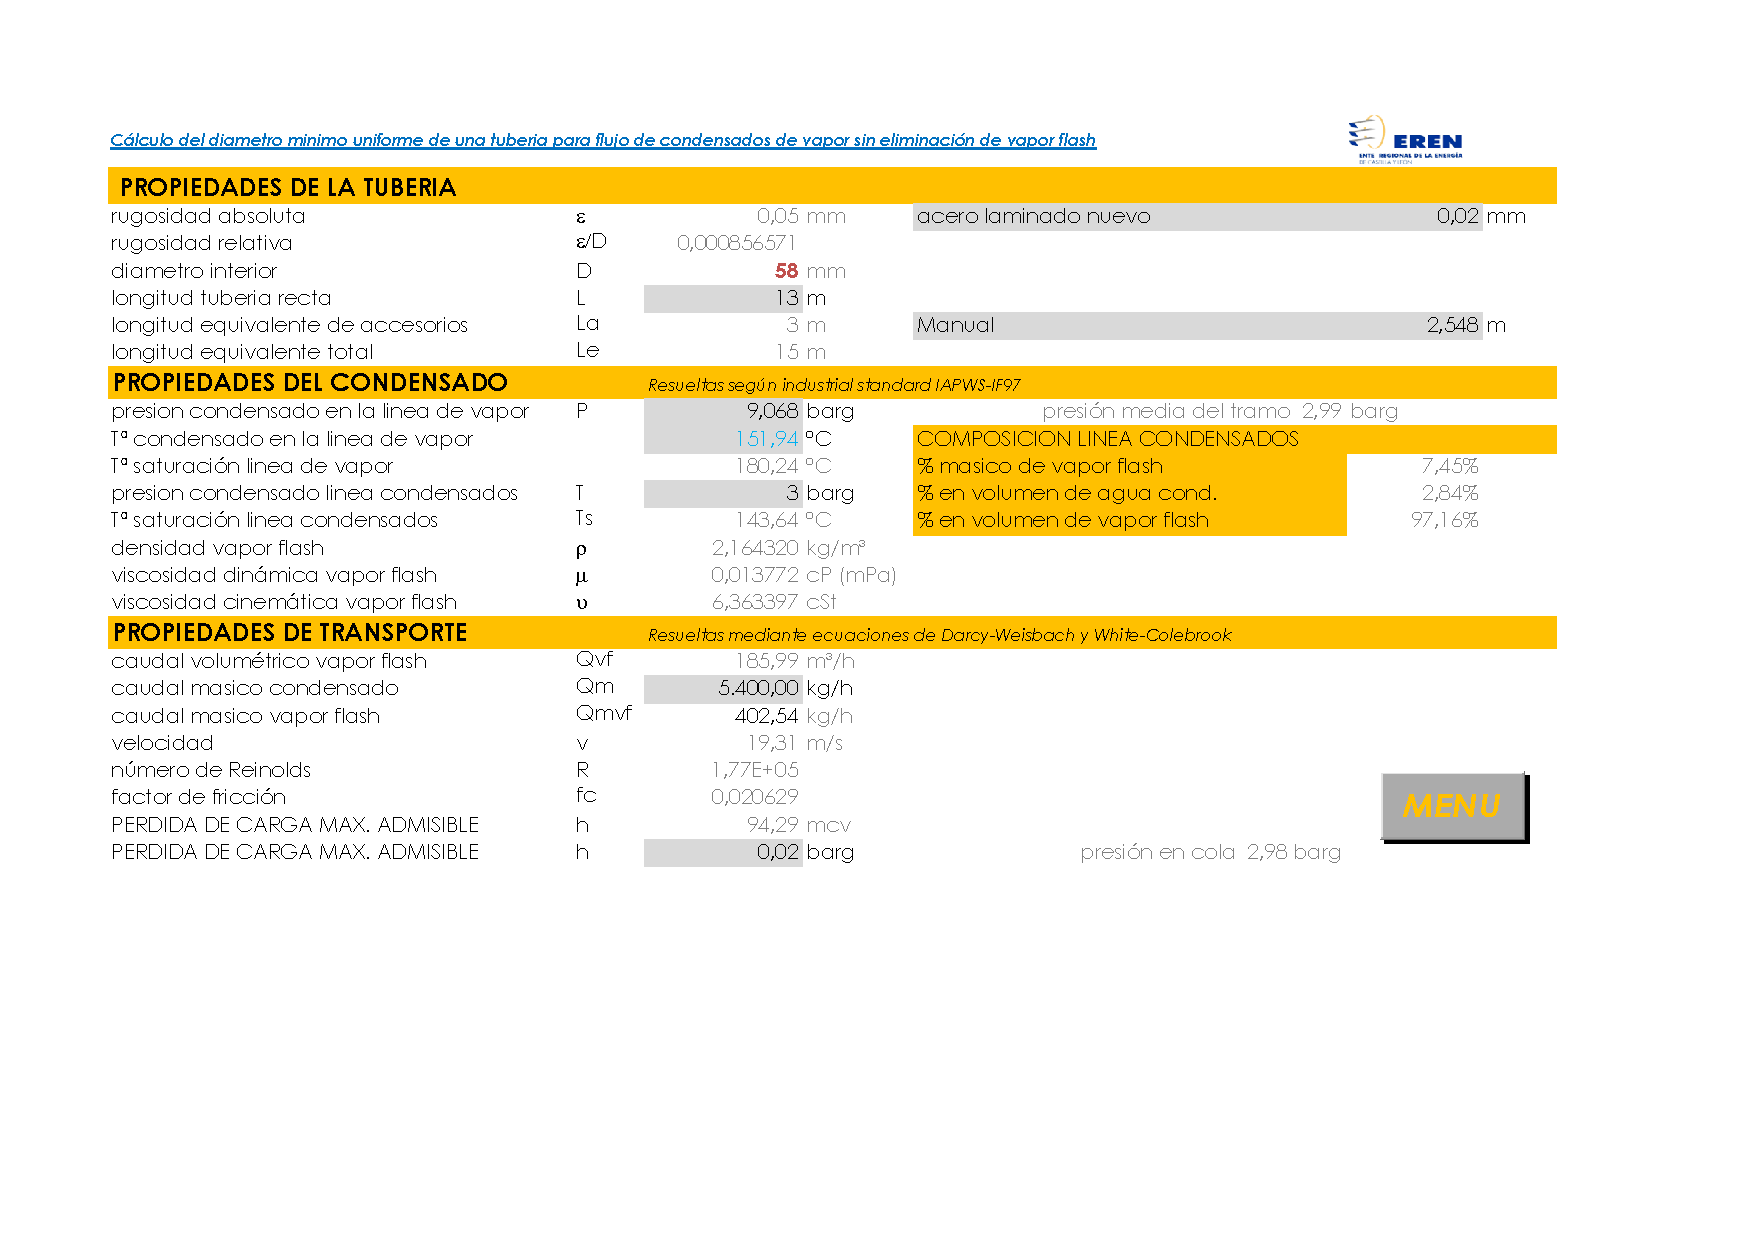
\includegraphics[width=0.95\textwidth]{Figuras/calculos_tramos/Condensados_TR1_Caldera-P.pdf}
	\caption{Cálculos del tramo TR1 (Caldera -- P) de la red de condensados}
	\label{fig:condensados-TR1}
\end{figure}

\paragraph{Tramo TR2: P -- C$_1$}

\begin{figure}[H]
	\centering
	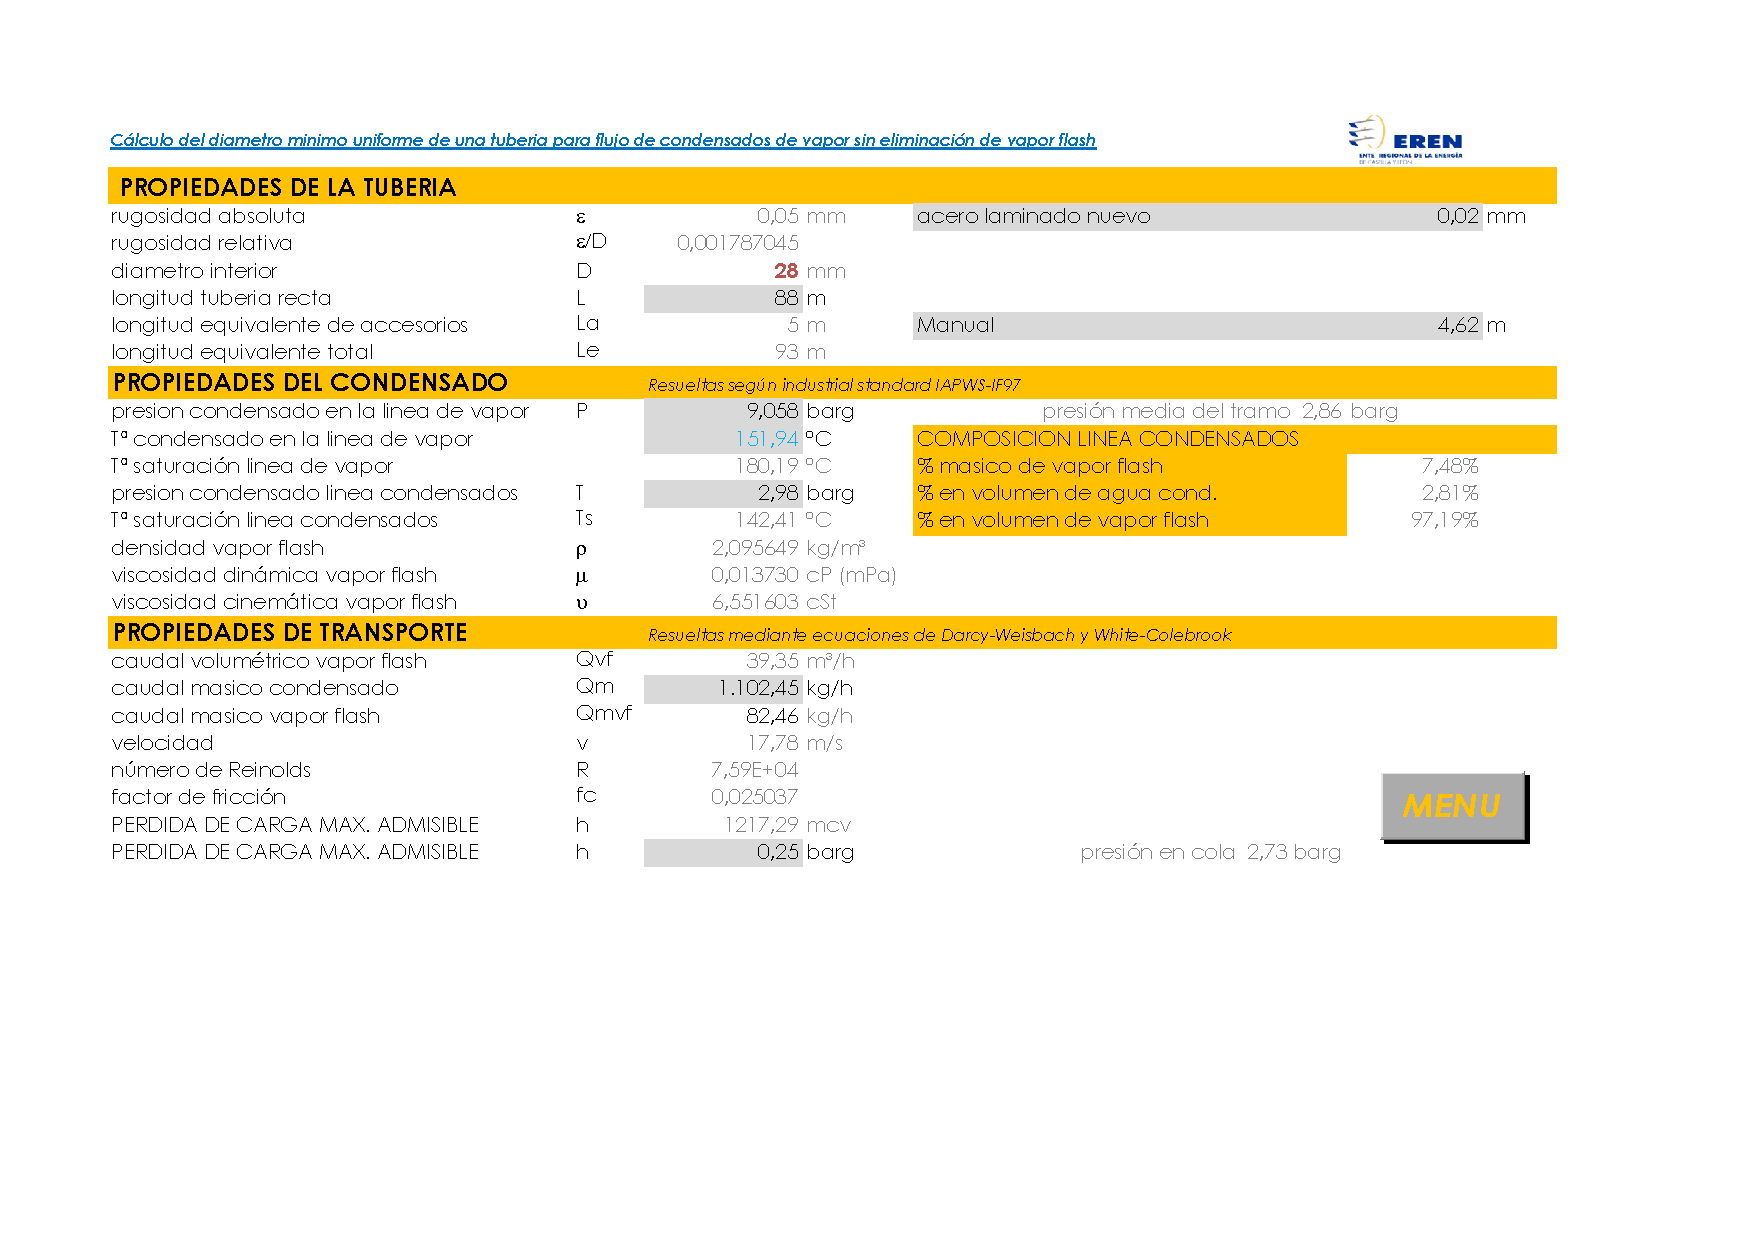
\includegraphics[width=0.95\textwidth]{Figuras/calculos_tramos/Condensados_TR2_P-C1.pdf}
	\caption{Cálculos del tramo TR2 (P -- C$_1$) de la red de condensados}
	\label{fig:condensados-TR2}
\end{figure}

\paragraph{Tramo TR3: P -- S}

\begin{figure}[H]
	\centering
	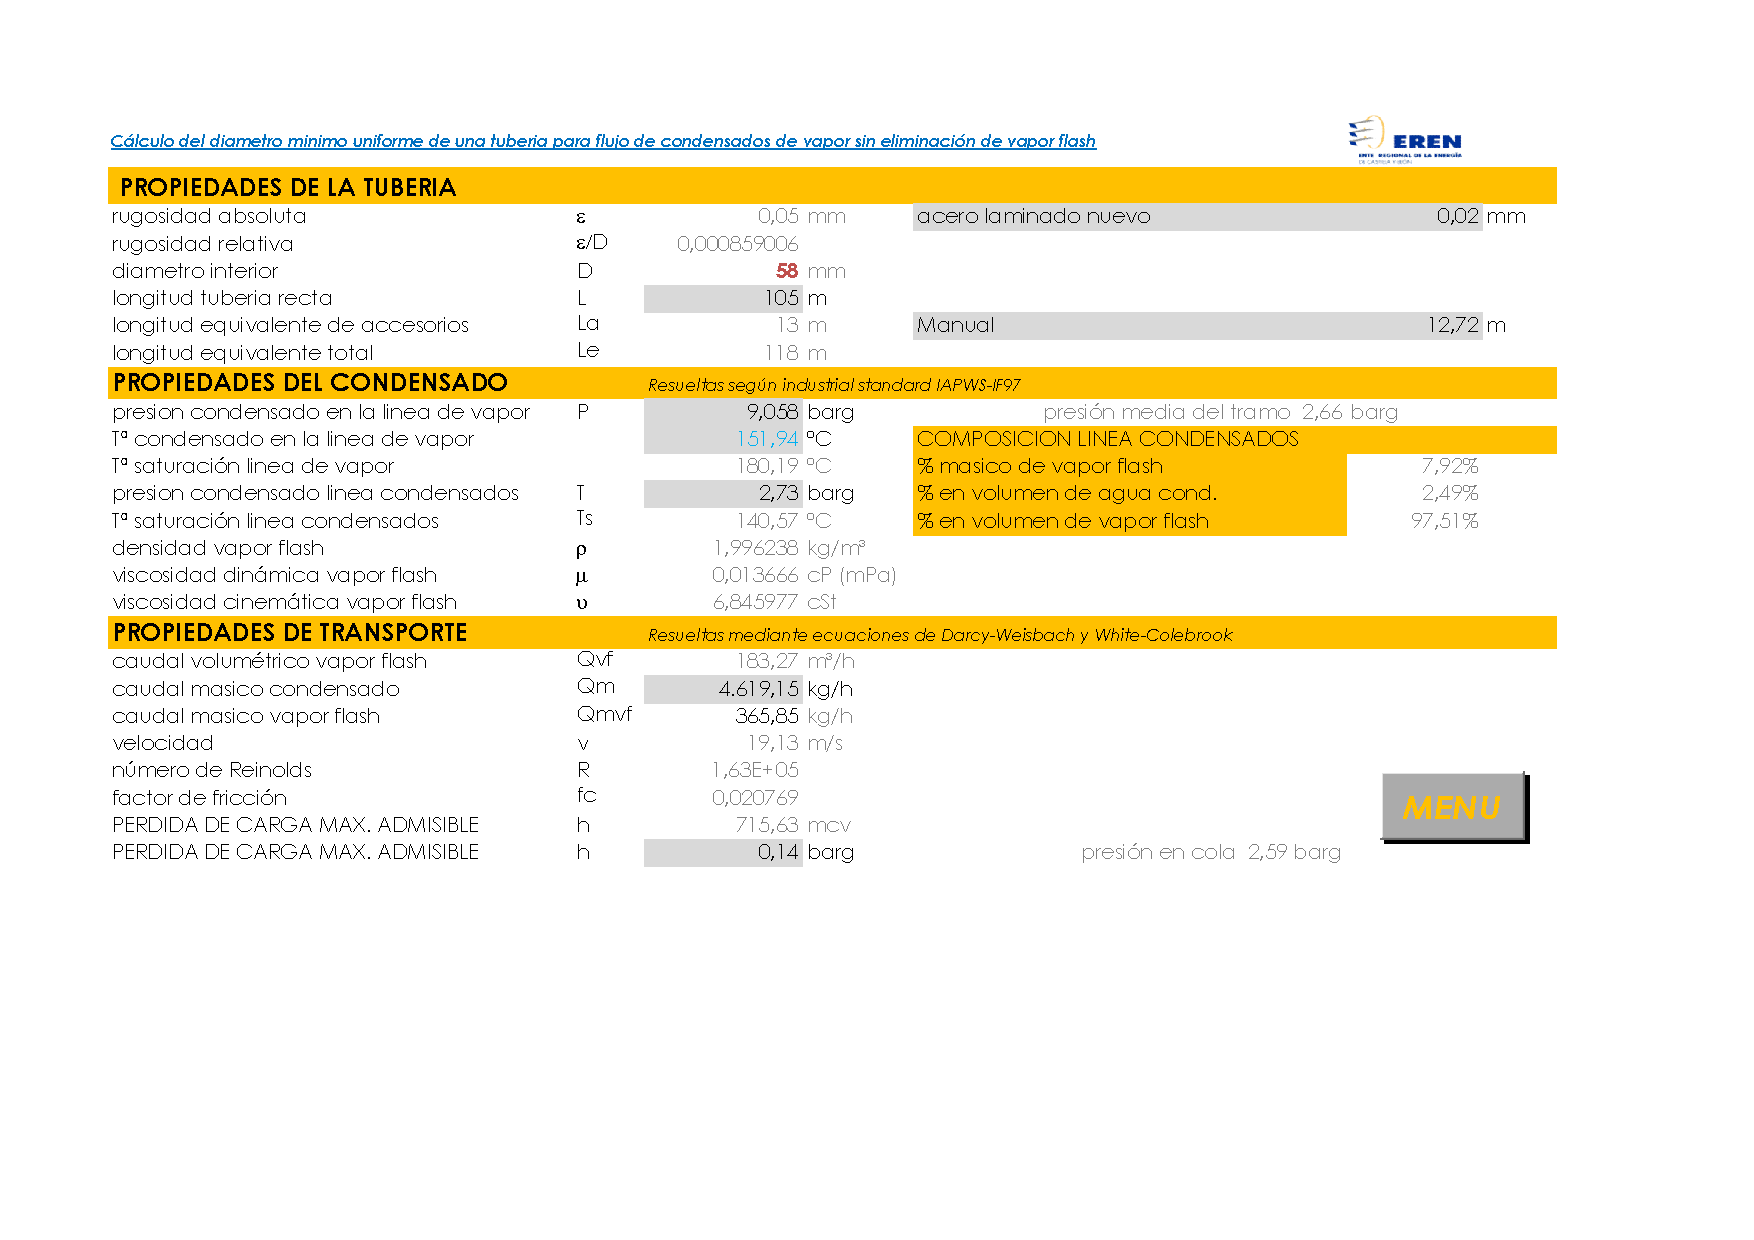
\includegraphics[width=0.95\textwidth]{Figuras/calculos_tramos/Condensados_TR3_P-S.pdf}
	\caption{Cálculos del tramo TR3 (P -- S) de la red de condensados}
	\label{fig:condensados-TR3}
\end{figure}

\paragraph{Tramo TR4: S -- C$_2$}

\begin{figure}[H]
	\centering
	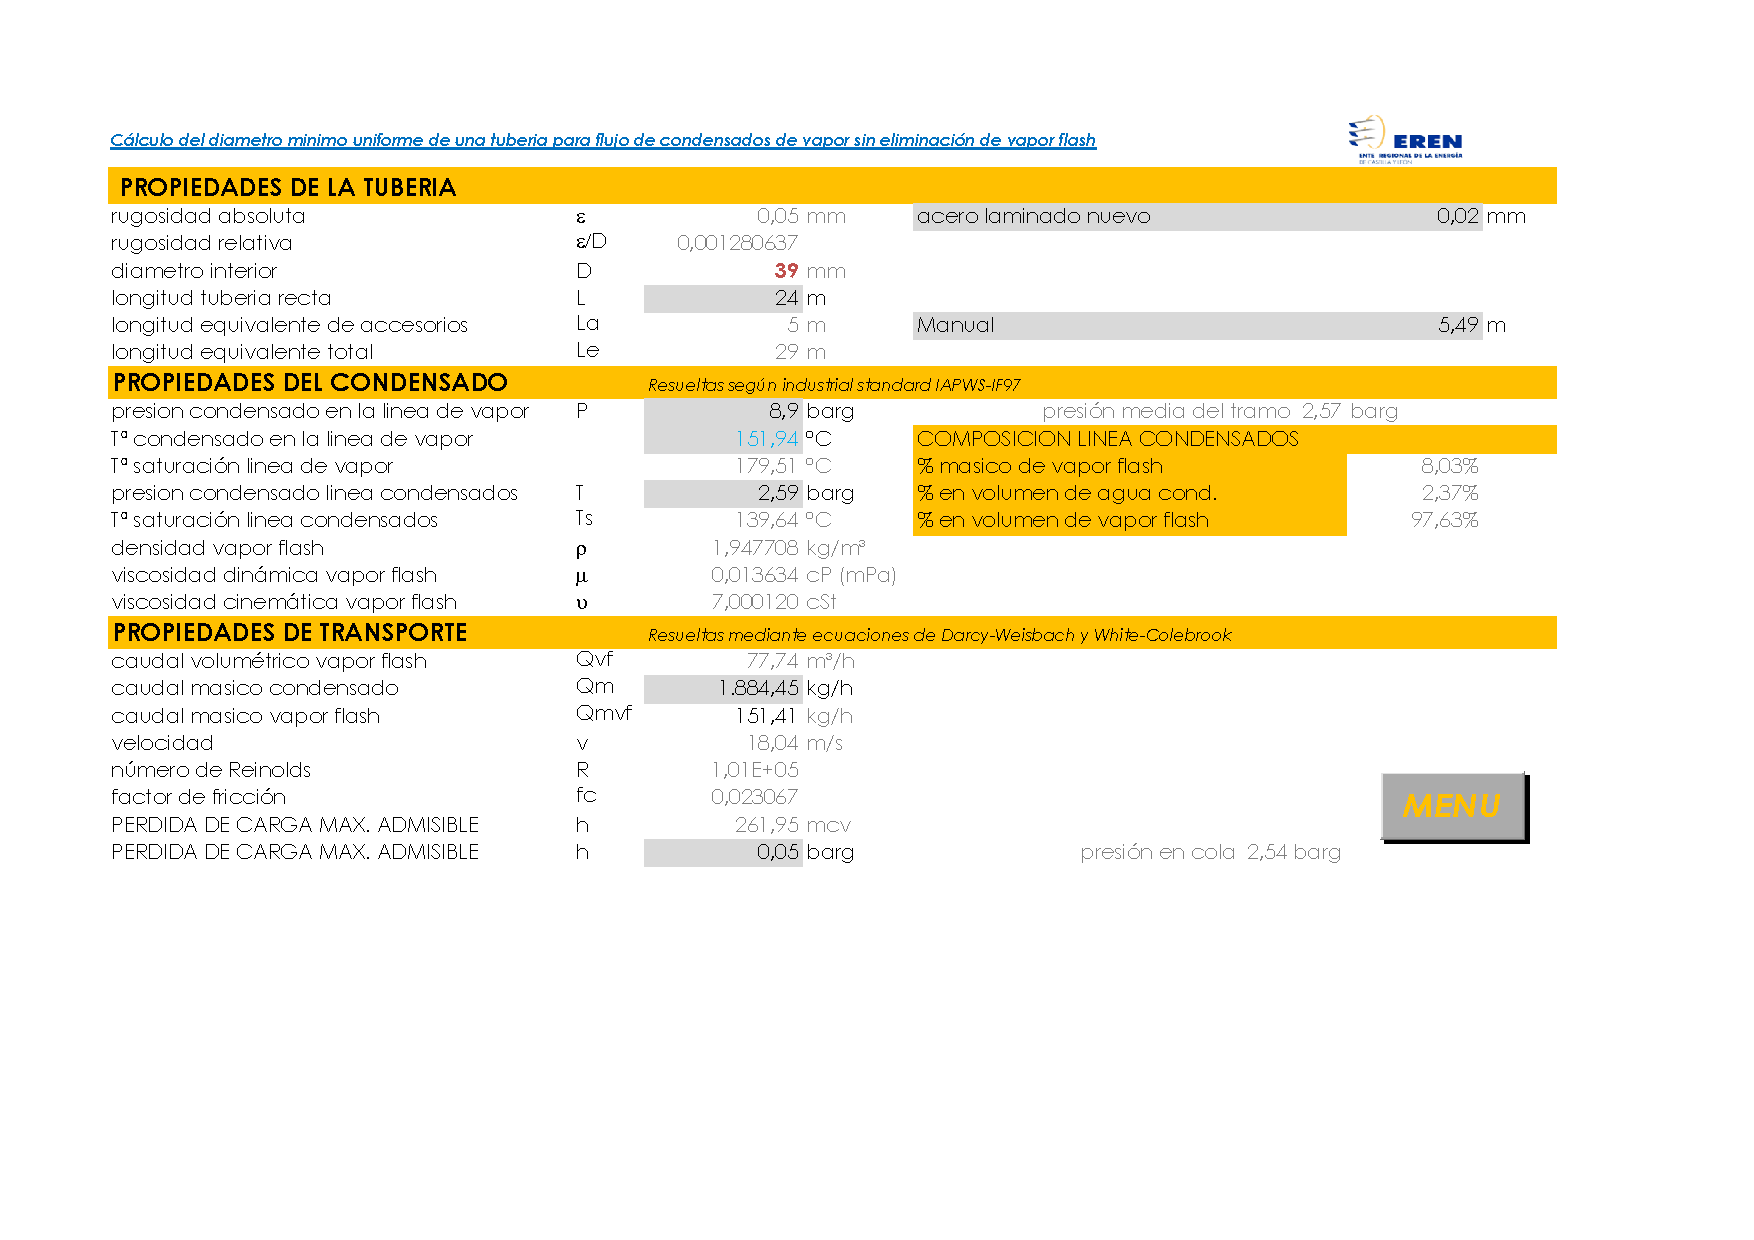
\includegraphics[width=0.95\textwidth]{Figuras/calculos_tramos/Condensados_TR4_S-C2.pdf}
	\caption{Cálculos del tramo TR4 (S -- C$_2$) de la red de condensados}
	\label{fig:condensados-TR4}
\end{figure}

\paragraph{Tramo TR5: S -- T}

\begin{figure}[H]
	\centering
	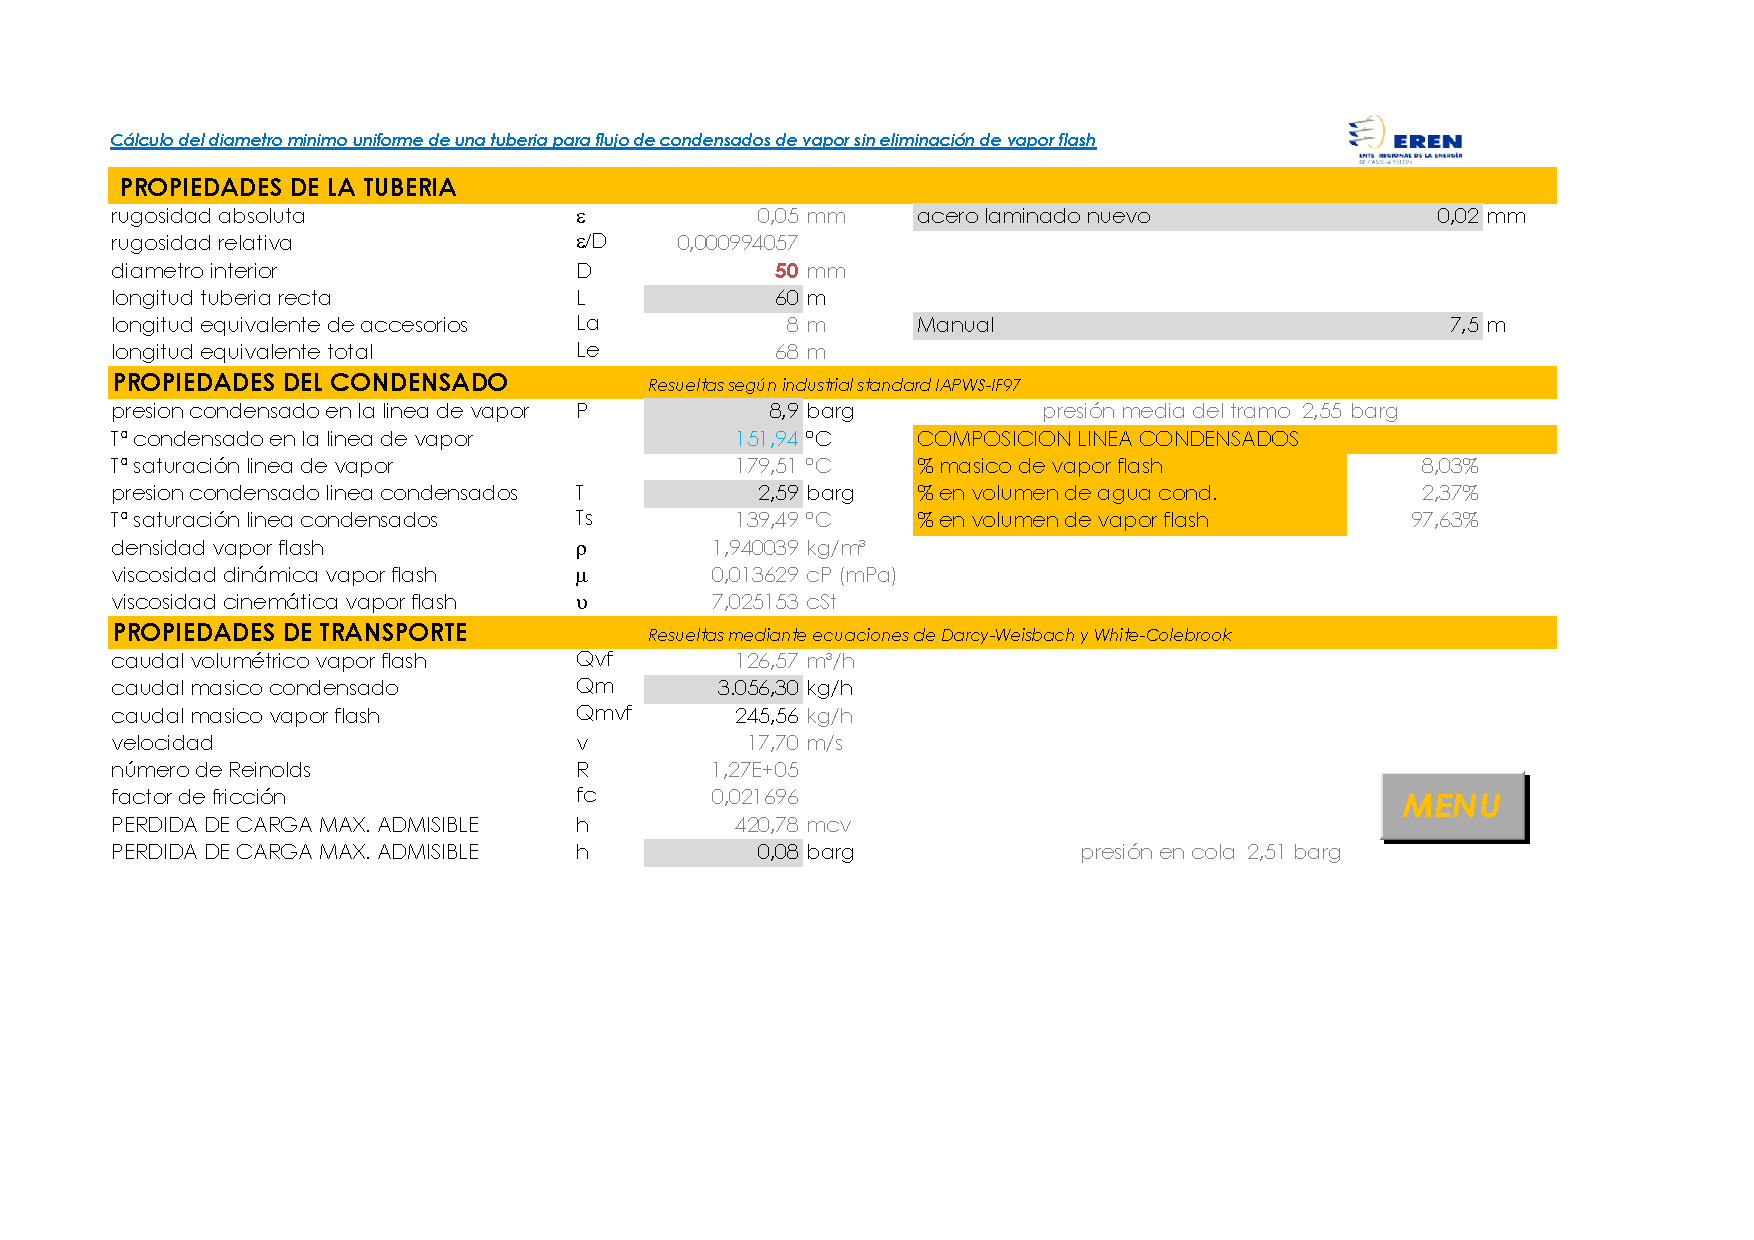
\includegraphics[width=0.95\textwidth]{Figuras/calculos_tramos/Condensados_TR5_S-T.pdf}
	\caption{Cálculos del tramo TR5 (S -- T) de la red de condensados}
	\label{fig:condensados-TR5}
\end{figure}

\paragraph{Tramo TR6: T -- C$_3$}

\begin{figure}[H]
	\centering
	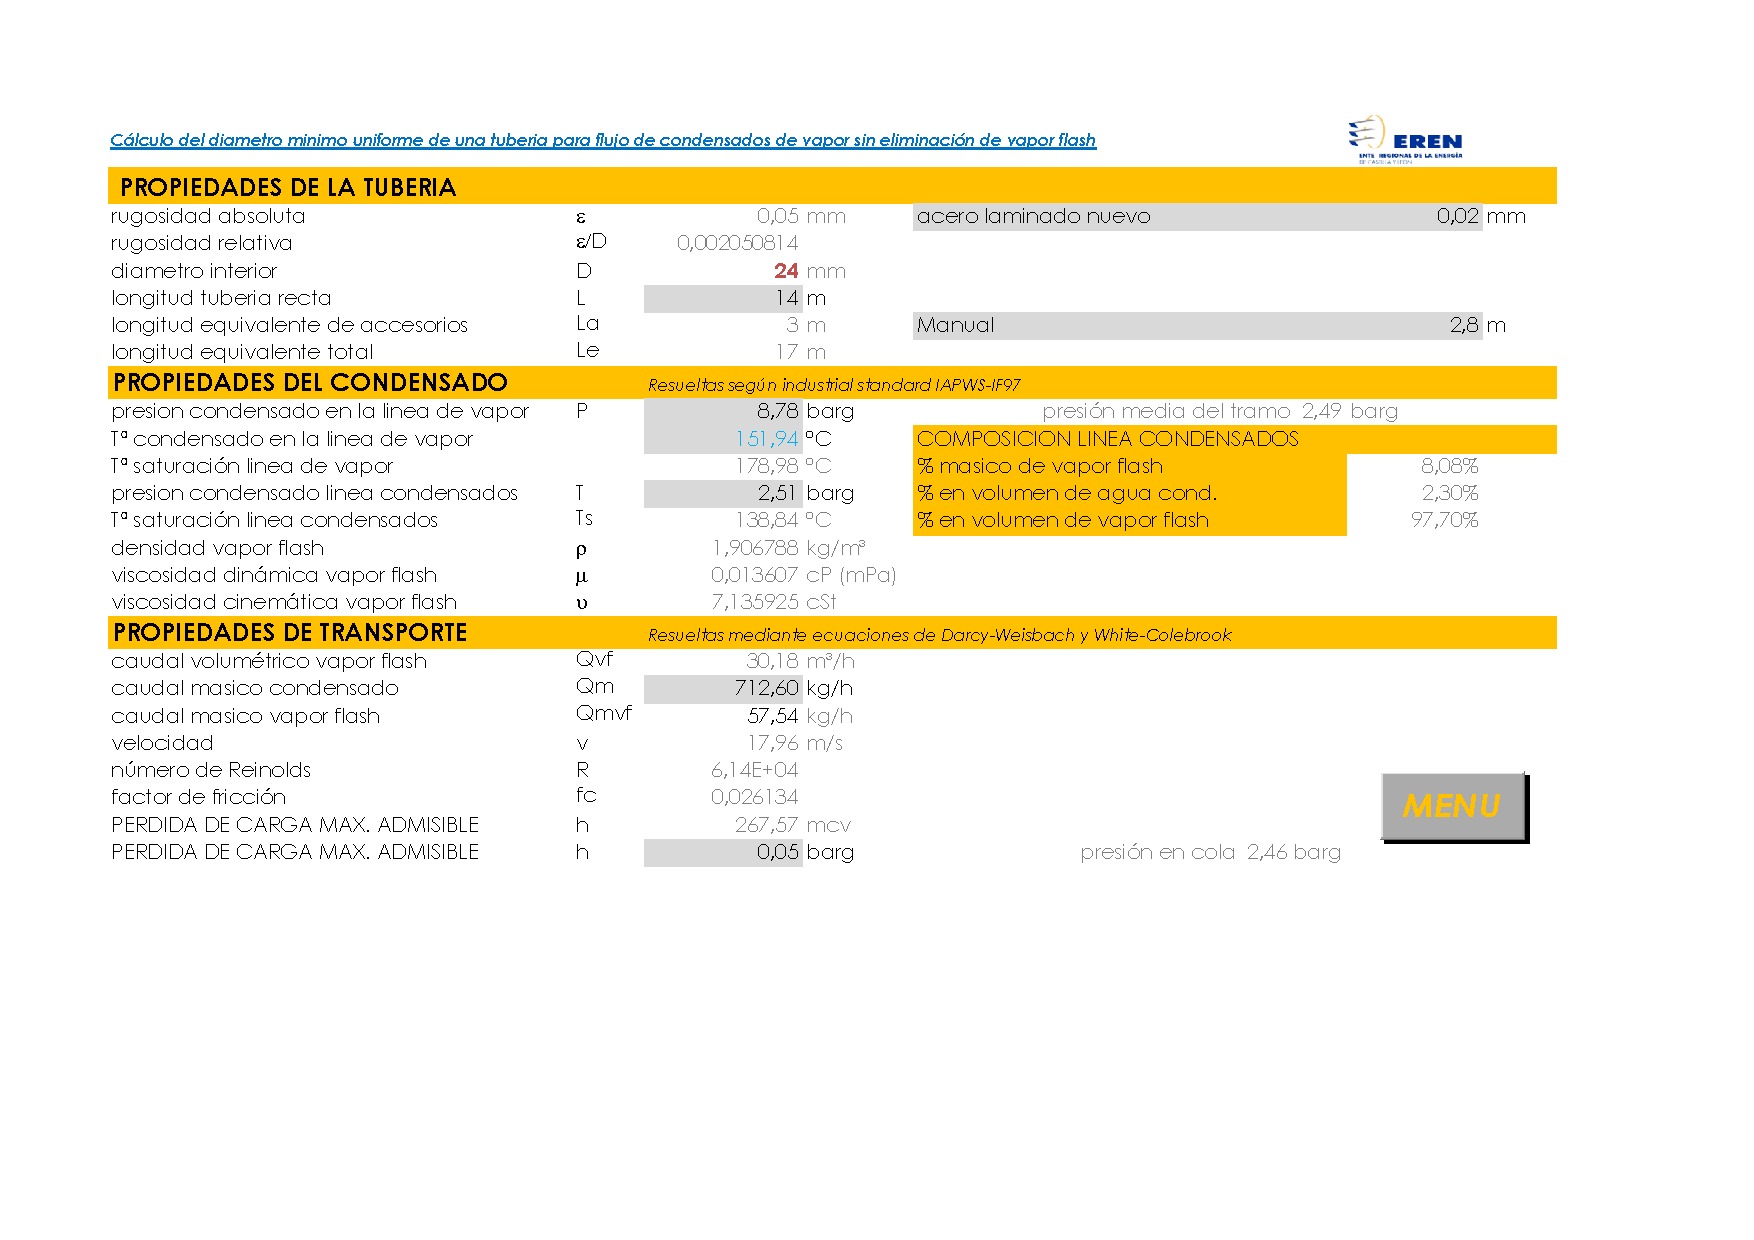
\includegraphics[width=0.95\textwidth]{Figuras/calculos_tramos/Condensados_TR6_T-C3.pdf}
	\caption{Cálculos del tramo TR6 (T -- C$_3$) de la red de condensados}
	\label{fig:condensados-TR6}
\end{figure}

\paragraph{Tramo TR7: T -- C$_4$}

\begin{figure}[H]
	\centering
	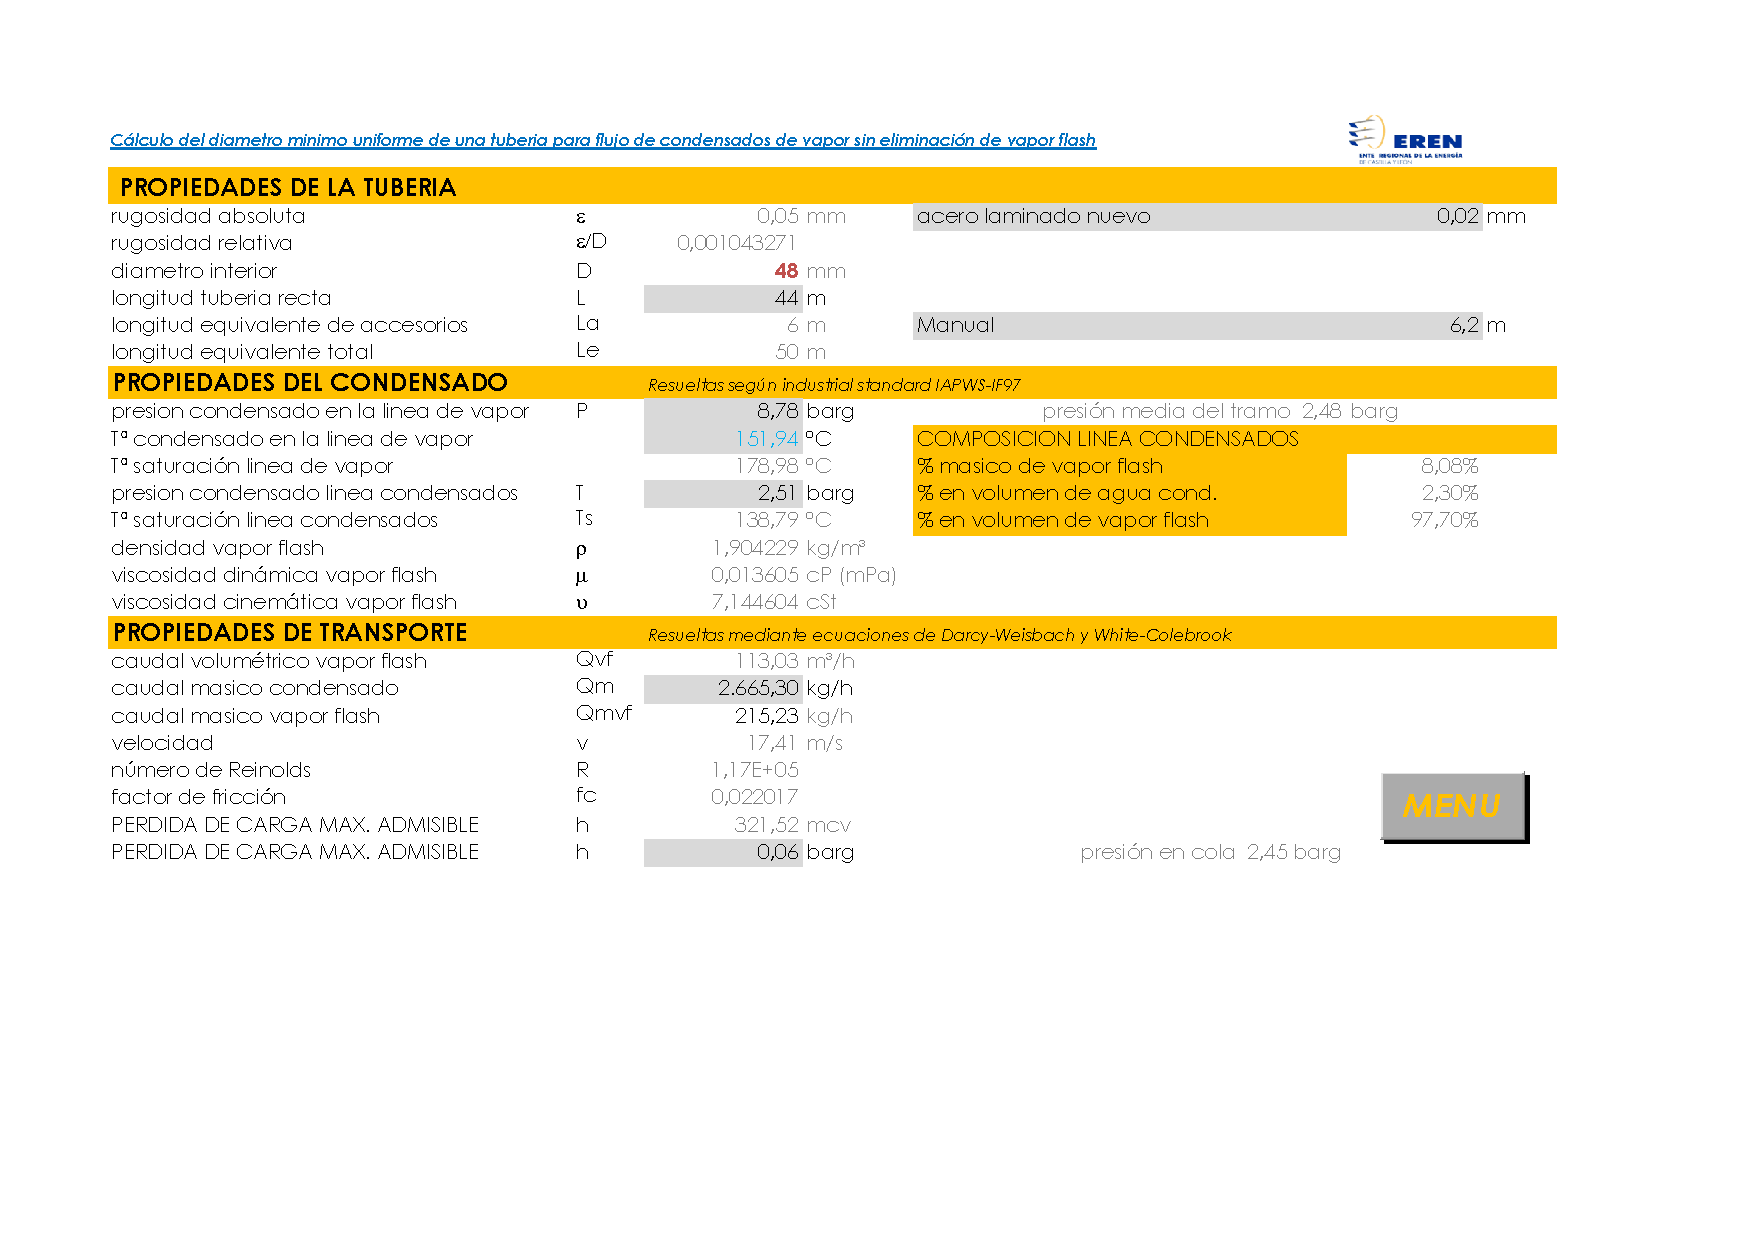
\includegraphics[width=0.95\textwidth]{Figuras/calculos_tramos/Condensados_TR7_T-C4.pdf}
	\caption{Cálculos del tramo TR7 (T -- C$_4$) de la red de condensados}
	\label{fig:condensados-TR7}
\end{figure}

\subsubsection{Resumen de la Red de Condensados}
\label{subsubsec:resumen-condensados}

\paragraph{Verificación de criterios de diseño}

La \tabref{tab:verificacion-condensados} presenta la verificación de los criterios de diseño para todos los tramos de la red de condensados.

\begin{table}[H]
	\centering
	\caption{Verificación de criterios de diseño en la red de condensados}
	\label{tab:verificacion-condensados}
	\begin{tabular}{ccccc}
		\toprule
		\textbf{Tramo} & \textbf{$v$ (m/s)} & \textbf{Criterio 15--20 m/s} & \textbf{$\Delta P$ (bar)} & \textbf{Estado} \\
		\midrule
		TR1            & 19{,}31            & \checkmark                   & 0{,}02                    & OK              \\
		TR2            & 17{,}78            & \checkmark                   & 0{,}25                    & OK              \\
		TR3            & 19{,}13            & \checkmark                   & 0{,}14                    & OK              \\
		TR4            & 18{,}04            & \checkmark                   & 0{,}05                    & OK              \\
		TR5            & 17{,}70            & \checkmark                   & 0{,}08                    & OK              \\
		TR6            & 17{,}96            & \checkmark                   & 0{,}05                    & OK              \\
		TR7            & 17{,}41            & \checkmark                   & 0{,}06                    & OK              \\
		\bottomrule
	\end{tabular}
\end{table}

\paragraph{Pérdida de carga por recorrido crítico}

La pérdida de carga acumulada desde cada consumidor hasta la caldera se presenta en la \tabref{tab:perdidas-condensados}.

\begin{table}[H]
	\centering
	\caption{Pérdida de carga acumulada en los recorridos de condensados}
	\label{tab:perdidas-condensados}
	\begin{tabular}{lcc}
		\toprule
		\textbf{Recorrido}          & \textbf{$\Delta P_{total}$ (bar)}            & \textbf{Estado} \\
		\midrule
		Caldera $\rightarrow$ C$_1$ & $0{,}02 + 0{,}25 = 0{,}27$                   & \checkmark      \\
		Caldera $\rightarrow$ C$_2$ & $0{,}02 + 0{,}14 + 0{,}05 = 0{,}21$          & \checkmark      \\
		Caldera $\rightarrow$ C$_3$ & $0{,}02 + 0{,}14 + 0{,}08 + 0{,}05 = 0{,}29$ & \checkmark      \\
		Caldera $\rightarrow$ C$_4$ & $0{,}02 + 0{,}14 + 0{,}08 + 0{,}06 = 0{,}30$ & \checkmark      \\
		\midrule
		\textbf{Máxima}             & \textbf{0{,}30}                              & \checkmark      \\
		\bottomrule
	\end{tabular}
\end{table}

\paragraph{Conclusiones del dimensionado de condensados}

El dimensionado hidráulico de la red de condensados cumple satisfactoriamente con todos los criterios de diseño establecidos:

\begin{itemize}[noitemsep]
	\item Todas las velocidades se mantienen en el rango 17{,}41--19{,}31~m/s, dentro del criterio de 15--20~m/s para flujo bifásico.
	\item La pérdida de carga máxima acumulada (0{,}30~bar hasta C$_4$) es aceptable para la presión de operación de 3~bar(g).
	\item El porcentaje de vapor flash calculado (7{,}45\%) justifica el uso de criterios de flujo bifásico.
	\item Se recomienda la instalación de un tanque de revaporizado para aprovechar los 402{,}54~kg/h de vapor flash.
	\item La selección de tubería Schedule~40 garantiza resistencia adecuada a la corrosión.
\end{itemize}


%%%%%%%%%%%%%%%%%%%%%%%%%%%%%%%%%%%%%%%%%%%%%%%%%%%%%%%%%%%%%
%%% SECCIÓN 2.4: AISLAMIENTO TÉRMICO Y DETALLES DE INSTALACIÓN
%%%%%%%%%%%%%%%%%%%%%%%%%%%%%%%%%%%%%%%%%%%%%%%%%%%%%%%%%%%%%

\subsection{Aislamiento Térmico y Detalles de Instalación}
\label{subsec:aislamiento_termico}

El diseño del aislamiento térmico constituye un aspecto fundamental en la eficiencia energética, seguridad operacional y viabilidad económica de instalaciones de vapor. Un aislamiento adecuado minimiza las pérdidas térmicas hacia el ambiente, protege al personal de superficies calientes, previene la condensación prematura del vapor en las tuberías y reduce los costes operativos del sistema. Esta subsección desarrolla el dimensionado completo del aislamiento térmico para la red de distribución, tanto en tramos aéreos como en el tramo enterrado, aplicando criterios normativos y buenas prácticas de ingeniería.


\subsubsection{Criterios de Aislamiento Térmico}
\label{subsubsec:criterios_aislamiento}

El dimensionado del aislamiento térmico debe satisfacer simultáneamente tres objetivos:

\begin{enumerate}[noitemsep]
	\item \textbf{Eficiencia energética}: Minimizar las pérdidas térmicas durante el transporte de vapor y condensados.
	\item \textbf{Seguridad del personal}: Limitar la temperatura superficial del aislamiento para evitar riesgos de quemaduras en zonas accesibles.
	\item \textbf{Viabilidad económica}: Optimizar el espesor para equilibrar coste de inversión con ahorros energéticos.
\end{enumerate}

\paragraph{Condiciones de operación y ambientales}
\label{par:condiciones_operacion_aisl}

Las temperaturas de operación de los fluidos en la instalación son:

\begin{itemize}[noitemsep]
	\item \textbf{Red de vapor}: $T_{\text{vap}} = 220$~°C (vapor saturado a 21~bar(g)).
	\item \textbf{Red de condensados}: $T_{\text{cond}} = 143{,}6$~°C (condensado saturado a 3~bar(g)).
\end{itemize}

Las condiciones ambientales adoptadas para el cálculo son:

\begin{itemize}[noitemsep]
	\item \textbf{Ambiente exterior} (tramos aéreos): $T_{\text{amb}} = 15$~°C, coeficiente convectivo $h_{\text{ext}} = 25$~W/(m$^2\cdot$K).
	\item \textbf{Terreno} (tramo enterrado): $T_{\text{terr}} = 10$~°C, conductividad térmica $\lambda_{\text{terr}} = 1{,}2$~W/(m$\cdot$K).
\end{itemize}

\paragraph{Materiales seleccionados}
\label{par:materiales_aislamiento}

Los materiales considerados en el cálculo térmico son:

\begin{itemize}[noitemsep]
	\item \textbf{Aislamiento térmico}: Lana de roca de alta densidad (120--150~kg/m$^3$), con conductividad térmica $\lambda_{\text{aisl}} = 0{,}04$~W/(m$\cdot$K) a temperatura media. Este material es ampliamente utilizado en instalaciones industriales por su excelente resistencia térmica, estabilidad dimensional a altas temperaturas y propiedades ignífugas.
	\item \textbf{Tubería}: Acero al carbono, con conductividad térmica $\lambda_{\text{acero}} = 50$~W/(m$\cdot$K).
\end{itemize}

\paragraph{Criterio normativo: RITE (RD 1027/2007)}
\label{par:criterio_rite}

El Reglamento de Instalaciones Térmicas en los Edificios (RITE) establece como criterio de seguridad que la temperatura superficial del aislamiento en zonas accesibles no supere los 30~°C, con el objetivo de eliminar el riesgo de quemaduras por contacto accidental. Este criterio se adopta como referencia para el dimensionado del espesor de aislamiento en tramos aéreos.

\paragraph{Modelo de transferencia de calor}
\label{par:modelo_transferencia}

El flujo de calor por unidad de longitud desde el fluido hacia el ambiente se calcula mediante la ecuación general de resistencias térmicas en serie:

\begin{equation}
	q_L = \frac{\Delta T}{\sum R}
	\label{eq:perdida_lineal_aisl}
\end{equation}

\noindent donde $\Delta T$ es la diferencia de temperatura entre el fluido y el ambiente, y $\sum R$ es la resistencia térmica total del sistema por unidad de longitud.

Las resistencias térmicas de cada capa cilíndrica se expresan mediante las siguientes ecuaciones:

\begin{equation}
	R_{\text{pipe}} = \frac{\ln(r_1 / r_{\text{int}})}{2\pi \lambda_{\text{acero}}}
	\label{eq:resist_tuberia}
\end{equation}

\begin{equation}
	R_{\text{aisl}} = \frac{\ln(r_2 / r_1)}{2\pi \lambda_{\text{aisl}}}
	\label{eq:resist_aislamiento}
\end{equation}

\begin{equation}
	R_{\text{surf}} = \frac{1}{\pi d_e h_{\text{ext}}}
	\label{eq:resist_superficie}
\end{equation}

\noindent donde $r_{\text{int}}$ es el radio interior de la tubería, $r_1$ es el radio exterior de la tubería, $r_2$ es el radio exterior del aislamiento, y $d_e = 2r_2$ es el diámetro exterior del conjunto aislado.

Para tramos enterrados, se añade la resistencia térmica del terreno, modelada mediante la ecuación de cilindro enterrado:

\begin{equation}
	R_{\text{terr}} = \frac{\ln(2 h_{\text{eje}} / r_2)}{2\pi \lambda_{\text{terr}}}
	\label{eq:resist_terreno}
\end{equation}

\noindent donde $h_{\text{eje}}$ es la profundidad del eje de la tubería respecto a la superficie del terreno. Adicionalmente, la resistencia térmica de la canalización (arena envolvente) se estima como $R_{\text{can}} \approx 0{,}05$~m$\cdot$K/W, valor típico para lechos de arena compactada.

Es importante destacar que, debido a la baja conductividad térmica del material aislante ($\lambda_{\text{aisl}} = 0{,}04$~W/(m$\cdot$K)), la resistencia del aislamiento $R_{\text{aisl}}$ es la resistencia dominante del sistema, representando típicamente más del 85\% de la resistencia térmica total. Las resistencias de la pared metálica ($R_{\text{pipe}}$) y de la superficie exterior ($R_{\text{surf}}$) tienen contribuciones menores pero no despreciables.


\subsubsection{Aislamiento de Tuberías Aéreas}
\label{subsubsec:aislamiento_aereo}

El diseño del aislamiento para los tramos aéreos de la instalación se basa en criterios de estandarización que permiten agrupar tuberías de diámetros nominales similares en rangos con espesor de aislamiento común. Esta estrategia, recomendada por guías de eficiencia energética (IDAE, ISO 12241) y fabricantes especializados (Isover, Spirax Sarco), presenta múltiples ventajas:

\begin{itemize}[noitemsep]
	\item \textbf{Reducción de costes logísticos}: Menor variedad de productos a adquirir y almacenar.
	\item \textbf{Simplificación de inventario}: Facilita la gestión de materiales en obra y mantenimiento.
	\item \textbf{Facilidad de instalación}: Los operarios trabajan con un número limitado de espesores estándar.
	\item \textbf{Mantenimiento predictivo}: La estandarización facilita la reposición de tramos dañados.
\end{itemize}

\paragraph{Criterios de estandarización por rangos de DN}
\label{par:rangos_estandarizados}

Los espesores de aislamiento seleccionados para la instalación, agrupados por rangos de diámetro nominal y tipo de red, se presentan en la \tabref{tab:rangos_estandarizados}.

\begin{table}[htbp]
	\centering
	\caption{Espesores de aislamiento estandarizados por rango de DN y tipo de red.}
	\label{tab:rangos_estandarizados}
	\begin{tabular}{lccc}
		\toprule
		\textbf{Red}             & \textbf{Rango DN (mm)} & \textbf{Espesor aislamiento (mm)} \\
		\midrule
		Vapor (220~°C)           & DN $\geq$ 125          & 100                               \\
		                         & DN 50--100             & 80                                \\
		                         & DN $<$ 50              & 60                                \\
		\midrule
		Condensados (143{,}6~°C) & DN $\geq$ 50           & 50                                \\
		                         & DN $<$ 50              & 40                                \\
		\bottomrule
	\end{tabular}
\end{table}

Estos espesores han sido verificados mediante cálculo térmico iterativo para garantizar el cumplimiento del criterio RITE ($T_{\text{surf}} \leq 30$~°C) en todos los tramos aéreos, con un margen de seguridad adecuado.

\paragraph{Resultados del dimensionado: Red de vapor}
\label{par:resultados_vapor_aereo}

La \tabref{tab:aislamiento_vapor_aereo} presenta el resumen completo del aislamiento térmico para los tramos aéreos de la red de vapor. Los cálculos se realizaron aplicando las ecuaciones \eqref{eq:perdida_lineal_aisl} a \eqref{eq:resist_superficie}, con las resistencias térmicas calculadas para cada diámetro y espesor de aislamiento.

\begin{table}[htbp]
	\centering
	\caption{Dimensionado de aislamiento térmico para tramos aéreos de la red de vapor.}
	\label{tab:aislamiento_vapor_aereo}
	\begin{tabular}{lcccccc}
		\toprule
		\textbf{Tramo}           & \textbf{DN (mm)} & \textbf{$L$ (m)}  & \textbf{$e_{\text{aisl}}$ (mm)} & \textbf{$q_L$ (W/m)} & \textbf{$Q$ (W)} \\
		\midrule
		TR1 (Caldera--P)         & 150              & 12{,}74           & 100                             & 65{,}1               & 829              \\
		TR3 (P--S)               & 125              & 106{,}00          & 100                             & 57{,}9               & 6\,137           \\
		TR4 (S--C$_2$)           & 80               & 25{,}00           & 80                              & 49{,}4               & 1\,235           \\
		TR5 (S--T)               & 100              & 60{,}00           & 80                              & 58{,}1               & 3\,486           \\
		TR6 (T--C$_3$)           & 50               & 15{,}00           & 80                              & 39{,}3               & 590              \\
		TR7 (T--C$_4$)           & 100              & 45{,}00           & 80                              & 58{,}1               & 2\,615           \\
		\midrule
		\textbf{TOTAL RED VAPOR} & ---              & \textbf{263{,}74} & ---                             & ---                  & \textbf{14\,892} \\
		\bottomrule
	\end{tabular}
	\vspace{0.3cm}

	\noindent \small \textit{Nota}: El tramo TR2 (P--C$_1$) es soterrado y se analiza específicamente en la sección 2.4.3.
\end{table}

Las pérdidas térmicas totales en los tramos aéreos de vapor alcanzan 14{,}89~kW, con una pérdida lineal promedio de 56{,}5~W/m. La temperatura superficial del aislamiento en todos los tramos se encuentra en el rango 17{,}1--18{,}2~°C, cumpliendo ampliamente con el criterio RITE de $T_{\text{surf}} < 30$~°C y con una diferencia inferior a 5~°C respecto a la temperatura ambiente, lo que elimina completamente el riesgo de quemaduras.

\paragraph{Resultados del dimensionado: Red de condensados}
\label{par:resultados_cond_aereo}

La \tabref{tab:aislamiento_cond_aereo} presenta el dimensionado del aislamiento para los tramos aéreos de la red de retorno de condensados. Aunque la temperatura de los condensados es significativamente inferior a la del vapor (143{,}6~°C frente a 220~°C), el aislamiento sigue siendo necesario para prevenir pérdidas energéticas y mantener la temperatura de retorno a caldera.

\begin{table}[htbp]
	\centering
	\caption{Dimensionado de aislamiento térmico para tramos aéreos de la red de condensados.}
	\label{tab:aislamiento_cond_aereo}
	\begin{tabular}{lcccccc}
		\toprule
		\textbf{Tramo}                 & \textbf{DN (mm)} & \textbf{$L$ (m)}  & \textbf{$e_{\text{aisl}}$ (mm)} & \textbf{$q_L$ (W/m)} & \textbf{$Q$ (W)} \\
		\midrule
		TR1 (Caldera--P)               & 65               & 12{,}74           & 50                              & 36{,}7               & 468              \\
		TR3 (P--S)                     & 65               & 105{,}00          & 50                              & 36{,}7               & 3\,854           \\
		TR4 (S--C$_2$)                 & 40               & 24{,}00           & 40                              & 32{,}3               & 775              \\
		TR5 (S--T)                     & 50               & 60{,}00           & 50                              & 32{,}4               & 1\,944           \\
		TR6 (T--C$_3$)                 & 25               & 14{,}00           & 40                              & 25{,}8               & 361              \\
		TR7 (T--C$_4$)                 & 50               & 44{,}00           & 50                              & 32{,}4               & 1\,426           \\
		\midrule
		\textbf{TOTAL RED CONDENSADOS} & ---              & \textbf{259{,}74} & ---                             & ---                  & \textbf{8\,828}  \\
		\bottomrule
	\end{tabular}
	\vspace{0.3cm}

	\noindent \small \textit{Nota}: El tramo TR2 (P--C$_1$) es soterrado y se analiza específicamente en la sección 2.4.3.
\end{table}

Las pérdidas térmicas totales en los tramos aéreos de condensados son de 8{,}83~kW, con una pérdida lineal promedio de 34{,}0~W/m. Las temperaturas superficiales resultantes se sitúan en el rango 16{,}3--17{,}8~°C, garantizando condiciones de seguridad óptimas.


\subsubsection{Análisis Especial: Tramo Enterrado (P--C$_1$)}
\label{subsubsec:tramo_enterrado}

El tramo TR2, que conecta el punto de patio (P) con el consumidor C$_1$, discurre enterrado bajo una zona de tránsito vehicular ocasional. Esta condición de instalación requiere un análisis térmico diferenciado, ya que el terreno circundante actúa como sumidero térmico adicional, modificando sustancialmente las condiciones de disipación de calor respecto a los tramos aéreos. Además, las restricciones geométricas impuestas por la profundidad de excavación y la necesidad de protección mecánica condicionan el espesor máximo de aislamiento aplicable.

\paragraph{Condiciones del Terreno y Profundidad de Enterramiento}
\label{par:condiciones_terreno}

El terreno donde se ejecuta la excavación presenta las siguientes propiedades térmicas:

\begin{itemize}[noitemsep]
	\item Conductividad térmica: $\lambda_{\text{terr}} = 1{,}2$~W/(m$\cdot$K) (terreno compacto con humedad media).
	\item Temperatura del terreno no perturbado: $T_{\text{terr}} = 10$~°C.
\end{itemize}

La profundidad del eje de las tuberías ($h_{\text{eje}}$) se determina a partir de la morfología de la zanja y los requerimientos de protección mecánica. La composición de capas desde la superficie hasta el eje de la tubería es la siguiente:

\begin{enumerate}[noitemsep]
	\item \textbf{Capa de relleno y zahorras}: 0{,}80~m (absorción de cargas dinámicas del tráfico).
	\item \textbf{Losa de hormigón HA-25}: 0{,}10~m (protección mecánica directa de las tuberías).
	\item \textbf{Margen de seguridad}: 0{,}10~m (distancia desde la losa hasta la superficie del aislamiento).
	\item \textbf{Radio exterior del aislamiento}: Para la tubería de vapor DN~80 con espesor de aislamiento de 50~mm, el radio exterior es $r_2 = 94{,}45$~mm $= 0{,}09445$~m.
\end{enumerate}

La profundidad total del eje de la tubería se calcula como:

\begin{equation}
	h_{\text{eje}} = 0{,}80 + 0{,}10 + 0{,}10 + r_2 = 0{,}80 + 0{,}10 + 0{,}10 + 0{,}09445 = 1{,}09445 \approx 1{,}09~\text{m}
	\label{eq:profundidad_eje}
\end{equation}

Esta profundidad es adecuada para garantizar protección mecánica y estabilidad térmica del terreno circundante.

\paragraph{Diseño de la Canalización y Morfología de la Zanja}
\label{par:diseno_canalizacion}

La zanja de enterramiento se diseña con geometría rectangular de sección constante, con las siguientes dimensiones:

\begin{itemize}[noitemsep]
	\item \textbf{Ancho total}: $B = 1{,}50$~m.
	\item \textbf{Profundidad total}: $H = 1{,}34$~m (desde superficie hasta fondo del lecho de arena).
	\item \textbf{Separación horizontal entre ejes}: 1{,}00~m (tubería de vapor y tubería de condensado).
\end{itemize}

Los diámetros exteriores de los conjuntos aislados son:

\begin{itemize}[noitemsep]
	\item \textbf{Tubería de vapor} (DN~80): $d_{e,\text{vap}} = 88{,}9 + 2 \times 50 = 188{,}9$~mm.
	\item \textbf{Tubería de condensado} (DN~32): $d_{e,\text{cond}} = 42{,}4 + 2 \times 40 = 122{,}4$~mm.
\end{itemize}

La morfología estratigráfica de la zanja, detallada en la \tabref{tab:morfologia_zanja}, combina capas de protección mecánica con materiales de relleno elástico que garantizan drenaje adecuado y transmisión controlada de cargas.

\begin{table}[htbp]
	\centering
	\caption{Morfología estratigráfica de la zanja de enterramiento.}
	\label{tab:morfologia_zanja}
	\begin{tabular}{lccclp{5cm}}
		\toprule
		\textbf{Capa}           & \textbf{Cota inicio} & \textbf{Cota fin} & \textbf{Espesor} & \textbf{Material}    & \textbf{Función}              \\
		\midrule
		1. Relleno              & $\pm 0{,}00$         & $-0{,}80$~m       & 0{,}80~m         & Zahorras compactadas & Absorción de cargas dinámicas \\
		2. Losa protección      & $-0{,}80$~m          & $-0{,}90$~m       & 0{,}10~m         & Hormigón HA-25       & Protección mecánica           \\
		3. Envolvente arena     & $-0{,}90$~m          & $-1{,}34$~m       & 0{,}44~m         & Arena de río lavada  & Lecho elástico, drenaje       \\
		\quad 3a. Margen sup.   & $-0{,}90$~m          & $-1{,}00$~m       & 0{,}10~m         & Arena lavada         & Zona de seguridad             \\
		\quad 3b. Zona tuberías & $-1{,}00$~m          & $-1{,}19$~m       & 0{,}19~m         & Arena + tuberías     & Eje a $-1{,}09$~m             \\
		\quad 3c. Lecho apoyo   & $-1{,}19$~m          & $-1{,}34$~m       & 0{,}15~m         & Arena nivelada       & Cama de apoyo (15~cm)         \\
		\bottomrule
	\end{tabular}
\end{table}

El esquema transversal de la zanja, mostrado en la \figref{fig:esquema_enterramiento}, ilustra la disposición relativa de las tuberías, la estructura de capas y las cotas de referencia.

\begin{figure}[htbp]
	\centering
	
\includegraphics[width=0.75\textwidth]{Figuras/esquema_enterramiento.pdf}
	\caption{Sección transversal de la zanja con disposición de tuberías y capas de protección.}
	\label{fig:esquema_enterramiento}
\end{figure}

La losa de hormigón HA-25 proporciona protección mecánica ante cargas vehiculares, mientras que la envolvente de arena actúa como material de relleno elástico que distribuye tensiones y facilita el drenaje de posibles infiltraciones de agua.

\paragraph{Cálculo de Resistencias Térmicas Combinadas}
\label{par:resistencias_termicas_combinadas}

El cálculo de las resistencias térmicas para el tramo enterrado incorpora tanto las resistencias del sistema tubería-aislamiento como las resistencias del entorno (canalización y terreno). A continuación se desarrollan los cálculos para ambas tuberías del tramo TR2.

\textbf{Tubería de vapor TR2 (DN~80, $e_{\text{aisl}} = 50$~mm)}

Geometría del sistema:

\begin{itemize}[noitemsep]
	\item Radio interior tubería: $r_{\text{int}} = 33{,}3$~mm $= 0{,}0333$~m.
	\item Radio exterior tubería: $r_1 = 44{,}45$~mm $= 0{,}04445$~m.
	\item Radio exterior aislamiento: $r_2 = r_1 + e_{\text{aisl}} = 44{,}45 + 50 = 94{,}45$~mm $= 0{,}09445$~m.
\end{itemize}

Aplicando la \eqref{eq:resist_tuberia}, la resistencia de la pared metálica es:

\begin{equation}
	R_{\text{pipe}} = \frac{\ln(0{,}04445 / 0{,}0333)}{2\pi \times 50} = \frac{0{,}2877}{314{,}16} = 0{,}0009~\text{m}\cdot\text{K/W}
	\label{eq:resist_pipe_TR2_vap}
\end{equation}

Aplicando la \eqref{eq:resist_aislamiento}, la resistencia del aislamiento es:

\begin{equation}
	R_{\text{aisl}} = \frac{\ln(0{,}09445 / 0{,}04445)}{2\pi \times 0{,}04} = \frac{0{,}7538}{0{,}2513} = 2{,}999~\text{m}\cdot\text{K/W}
	\label{eq:resist_aisl_TR2_vap}
\end{equation}

La resistencia de la canalización (arena envolvente) se adopta con el valor típico:

\begin{equation}
	R_{\text{can}} = 0{,}050~\text{m}\cdot\text{K/W}
	\label{eq:resist_can_TR2}
\end{equation}

Aplicando la \eqref{eq:resist_terreno}, la resistencia del terreno es:

\begin{equation}
	R_{\text{terr}} = \frac{\ln(2 \times 1{,}09 / 0{,}09445)}{2\pi \times 1{,}2} = \frac{\ln(23{,}08)}{7{,}540} = \frac{3{,}139}{7{,}540} = 0{,}417~\text{m}\cdot\text{K/W}
	\label{eq:resist_terr_TR2_vap}
\end{equation}

La resistencia térmica total para la tubería de vapor enterrada es:

\begin{equation}
	\sum R_{\text{tot,vap}} = R_{\text{pipe}} + R_{\text{aisl}} + R_{\text{can}} + R_{\text{terr}} = 0{,}0009 + 2{,}999 + 0{,}050 + 0{,}417 = \textbf{3{,}467}~\textbf{m}\cdot\textbf{K/W}
	\label{eq:resist_total_TR2_vap}
\end{equation}

\textbf{Tubería de condensado TR2 (DN~32, $e_{\text{aisl}} = 40$~mm)}

Geometría del sistema:

\begin{itemize}[noitemsep]
	\item Radio interior tubería: $r_{\text{int}} = 14{,}0$~mm $= 0{,}0140$~m.
	\item Radio exterior tubería: $r_1 = 21{,}2$~mm $= 0{,}0212$~m.
	\item Radio exterior aislamiento: $r_2 = r_1 + e_{\text{aisl}} = 21{,}2 + 40 = 61{,}2$~mm $= 0{,}0612$~m.
\end{itemize}

Resistencia de la pared metálica (despreciable):

\begin{equation}
	R_{\text{pipe}} = \frac{\ln(0{,}0212 / 0{,}0140)}{2\pi \times 50} = \frac{0{,}4143}{314{,}16} \approx 0{,}0008~\text{m}\cdot\text{K/W}
	\label{eq:resist_pipe_TR2_cond}
\end{equation}

Resistencia del aislamiento:

\begin{equation}
	R_{\text{aisl}} = \frac{\ln(0{,}0612 / 0{,}0212)}{2\pi \times 0{,}04} = \frac{1{,}0594}{0{,}2513} = 4{,}223~\text{m}\cdot\text{K/W}
	\label{eq:resist_aisl_TR2_cond}
\end{equation}

Resistencia de la canalización (mismo valor que vapor):

\begin{equation}
	R_{\text{can}} = 0{,}050~\text{m}\cdot\text{K/W}
	\label{eq:resist_can_TR2_cond}
\end{equation}

Resistencia del terreno (menor radio exterior implica mayor resistencia):

\begin{equation}
	R_{\text{terr}} = \frac{\ln(2 \times 1{,}09 / 0{,}0612)}{2\pi \times 1{,}2} = \frac{\ln(35{,}62)}{7{,}540} = \frac{3{,}573}{7{,}540} = 0{,}474~\text{m}\cdot\text{K/W}
	\label{eq:resist_terr_TR2_cond}
\end{equation}

La resistencia térmica total para la tubería de condensado enterrada es:

\begin{equation}
	\sum R_{\text{tot,cond}} = R_{\text{pipe}} + R_{\text{aisl}} + R_{\text{can}} + R_{\text{terr}} = 0{,}0008 + 4{,}223 + 0{,}050 + 0{,}474 = \textbf{4{,}747}~\textbf{m}\cdot\textbf{K/W}
	\label{eq:resist_total_TR2_cond}
\end{equation}

La \tabref{tab:resistencias_TR2} compara las contribuciones relativas de cada resistencia térmica para ambas tuberías del tramo enterrado.

\begin{table}[htbp]
	\centering
	\caption{Comparación de resistencias térmicas en el tramo enterrado TR2.}
	\label{tab:resistencias_TR2}
	\begin{tabular}{lcccc}
		\toprule
		\textbf{Resistencia} & \multicolumn{2}{c}{\textbf{Vapor DN~80}} & \multicolumn{2}{c}{\textbf{Condensado DN~32}}                                               \\
		\cmidrule(lr){2-3} \cmidrule(lr){4-5}
		                     & \textbf{Valor (m$\cdot$K/W)}             & \textbf{\%}                                   & \textbf{Valor (m$\cdot$K/W)} & \textbf{\%}  \\
		\midrule
		$R_{\text{pipe}}$    & 0{,}0009                                 & 0{,}03                                        & 0{,}0008                     & 0{,}02       \\
		$R_{\text{aisl}}$    & 2{,}999                                  & 86{,}51                                       & 4{,}223                      & 88{,}96      \\
		$R_{\text{can}}$     & 0{,}050                                  & 1{,}44                                        & 0{,}050                      & 1{,}05       \\
		$R_{\text{terr}}$    & 0{,}417                                  & 12{,}02                                       & 0{,}474                      & 9{,}98       \\
		\midrule
		\textbf{Total}       & \textbf{3{,}467}                         & \textbf{100}                                  & \textbf{4{,}747}             & \textbf{100} \\
		\bottomrule
	\end{tabular}
\end{table}

Como se observa en la \tabref{tab:resistencias_TR2}, el aislamiento térmico aporta aproximadamente el 87\% de la resistencia total en ambas tuberías, confirmando su papel dominante en la reducción de pérdidas térmicas. La resistencia del terreno tiene una contribución significativa (10--12\%), mientras que las resistencias de la pared metálica y la canalización son prácticamente despreciables.

\paragraph{Determinación del Espesor Óptimo y Pérdidas Térmicas del Tramo}
\label{par:espesor_optimo_perdidas}

Los espesores de aislamiento seleccionados para el tramo enterrado (50~mm para vapor, 40~mm para condensados) son inferiores a los espesores estándar adoptados en tramos aéreos de diámetros equivalentes (80~mm para DN~80 de vapor, 50~mm para DN~32 de condensado). Esta reducción responde a una restricción geométrica impuesta por la profundidad de enterramiento y el dimensionado de la zanja:

\begin{itemize}[noitemsep]
	\item Un espesor de aislamiento mayor en la tubería de vapor (p.~ej., 80~mm) incrementaría el radio exterior hasta $r_2 = 88{,}9/2 + 80 = 124{,}45$~mm, lo que requeriría aumentar la profundidad de excavación en aproximadamente 30~cm adicionales para mantener el margen de seguridad.
	\item Este incremento de profundidad elevaría sustancialmente los costes de excavación, contención de tierras y tiempo de ejecución.
	\item El análisis coste-beneficio favorece la solución con espesores reducidos, especialmente considerando que la resistencia térmica del terreno ($R_{\text{terr}}$) contribuye adicionalmente a limitar las pérdidas.
\end{itemize}

\textbf{Pérdidas térmicas en la tubería de vapor TR2}

Aplicando la \eqref{eq:perdida_lineal_aisl} con la resistencia total calculada en la \eqref{eq:resist_total_TR2_vap}:

\begin{equation}
	q_{L,\text{vap}} = \frac{T_{\text{vap}} - T_{\text{terr}}}{\sum R_{\text{tot,vap}}} = \frac{220 - 10}{3{,}467} = \frac{210}{3{,}467} = 60{,}6~\text{W/m}
	\label{eq:perdida_lineal_TR2_vap}
\end{equation}

La pérdida térmica total para la longitud del tramo de vapor ($L_{\text{vap}} = 88{,}19$~m) es:

\begin{equation}
	Q_{\text{vap,TR2}} = q_{L,\text{vap}} \times L_{\text{vap}} = 60{,}6 \times 88{,}19 = 5\,344~\text{W} \approx \textbf{5{,}34~kW}
	\label{eq:perdida_total_TR2_vap}
\end{equation}

\textbf{Pérdidas térmicas en la tubería de condensado TR2}

Aplicando la \eqref{eq:perdida_lineal_aisl} con la resistencia total calculada en la \eqref{eq:resist_total_TR2_cond}:

\begin{equation}
	q_{L,\text{cond}} = \frac{T_{\text{cond}} - T_{\text{terr}}}{\sum R_{\text{tot,cond}}} = \frac{143{,}6 - 10}{4{,}747} = \frac{133{,}6}{4{,}747} = 28{,}1~\text{W/m}
	\label{eq:perdida_lineal_TR2_cond}
\end{equation}

La pérdida térmica total para la longitud del tramo de condensado ($L_{\text{cond}} = 61{,}87$~m) es:

\begin{equation}
	Q_{\text{cond,TR2}} = q_{L,\text{cond}} \times L_{\text{cond}} = 28{,}1 \times 61{,}87 = 1\,739~\text{W} \approx \textbf{1{,}74~kW}
	\label{eq:perdida_total_TR2_cond}
\end{equation}

\textbf{Pérdida térmica total del tramo enterrado TR2}

La suma de las pérdidas térmicas de ambas tuberías resulta en:

\begin{equation}
	Q_{\text{TR2,total}} = Q_{\text{vap,TR2}} + Q_{\text{cond,TR2}} = 5{,}34 + 1{,}74 = \textbf{7{,}08~kW}
	\label{eq:perdida_total_TR2}
\end{equation}

Esta pérdida térmica, aunque superior en términos absolutos a tramos aéreos individuales de longitud similar, es aceptable considerando la longitud total del tramo enterrado (150{,}06~m combinados). Es importante observar que el tramo enterrado representa únicamente el 5{,}5\% de la longitud total de la instalación pero concentra aproximadamente el 23\% de las pérdidas térmicas totales, consecuencia directa del menor espesor de aislamiento aplicado.


\subsubsection{Cuadro Resumen de Espesores de Aislamiento para Toda la Instalación}
\label{subsubsec:resumen_aislamiento}

Esta subsección consolida los resultados del dimensionado térmico para la totalidad de la red de distribución, integrando tanto los tramos aéreos como el tramo enterrado. Las tablas siguientes constituyen el balance energético completo del sistema de aislamiento, permitiendo evaluar la eficiencia global del diseño.

\paragraph{Red de vapor: resumen completo}
\label{par:resumen_vapor_completo}

La \tabref{tab:resumen_vapor_completo} presenta el dimensionado de aislamiento para los siete tramos de la red de distribución de vapor, incluyendo el tramo soterrado TR2 con sus condiciones específicas de cálculo.

\begin{table}[htbp]
	\centering
	\caption{Dimensionado completo del aislamiento térmico para la red de distribución de vapor.}
	\label{tab:resumen_vapor_completo}
	\begin{tabular}{lcccccc}
		\toprule
		\textbf{Tramo}           & \textbf{Ubicación} & \textbf{DN (mm)} & \textbf{$L$ (m)}  & \textbf{$e_{\text{aisl}}$ (mm)} & \textbf{$q_L$ (W/m)} & \textbf{$Q$ (W)} \\
		\midrule
		TR1 (Caldera--P)         & Aéreo              & 150              & 12{,}74           & 100                             & 65{,}1               & 829              \\
		TR2 (P--C$_1$)           & \textbf{Soterrado} & 80               & 88{,}19           & 50                              & 60{,}6               & 5\,344           \\
		TR3 (P--S)               & Aéreo              & 125              & 106{,}00          & 100                             & 57{,}9               & 6\,137           \\
		TR4 (S--C$_2$)           & Aéreo              & 80               & 25{,}00           & 80                              & 49{,}4               & 1\,235           \\
		TR5 (S--T)               & Aéreo              & 100              & 60{,}00           & 80                              & 58{,}1               & 3\,486           \\
		TR6 (T--C$_3$)           & Aéreo              & 50               & 15{,}00           & 80                              & 39{,}3               & 590              \\
		TR7 (T--C$_4$)           & Aéreo              & 100              & 45{,}00           & 80                              & 58{,}1               & 2\,615           \\
		\midrule
		\textbf{TOTAL RED VAPOR} & ---                & ---              & \textbf{351{,}93} & ---                             & ---                  & \textbf{20\,236} \\
		\bottomrule
	\end{tabular}
	\vspace{0.3cm}

	\noindent \small \textit{Nota}: Las pérdidas térmicas totales de la red de vapor alcanzan \textbf{20{,}24~kW}.
\end{table}

El tramo enterrado TR2 destaca por su contribución significativa al balance térmico: con una longitud de 88{,}19~m (25{,}1\% de la red de vapor) y un espesor de aislamiento reducido, representa 5{,}34~kW de pérdidas, lo que equivale al 26{,}4\% de las pérdidas totales de la red de vapor.

\paragraph{Red de condensados: resumen completo}
\label{par:resumen_cond_completo}

La \tabref{tab:resumen_cond_completo} presenta el dimensionado de aislamiento para los siete tramos de la red de retorno de condensados, incluyendo el tramo soterrado TR2.

\begin{table}[htbp]
	\centering
	\caption{Dimensionado completo del aislamiento térmico para la red de retorno de condensados.}
	\label{tab:resumen_cond_completo}
	\begin{tabular}{lcccccc}
		\toprule
		\textbf{Tramo}                 & \textbf{Ubicación} & \textbf{DN (mm)} & \textbf{$L$ (m)}  & \textbf{$e_{\text{aisl}}$ (mm)} & \textbf{$q_L$ (W/m)} & \textbf{$Q$ (W)} \\
		\midrule
		TR1 (Caldera--P)               & Aéreo              & 65               & 12{,}74           & 50                              & 36{,}7               & 468              \\
		TR2 (P--C$_1$)                 & \textbf{Soterrado} & 32               & 61{,}87           & 40                              & 28{,}1               & 1\,739           \\
		TR3 (P--S)                     & Aéreo              & 65               & 105{,}00          & 50                              & 36{,}7               & 3\,854           \\
		TR4 (S--C$_2$)                 & Aéreo              & 40               & 24{,}00           & 40                              & 32{,}3               & 775              \\
		TR5 (S--T)                     & Aéreo              & 50               & 60{,}00           & 50                              & 32{,}4               & 1\,944           \\
		TR6 (T--C$_3$)                 & Aéreo              & 25               & 14{,}00           & 40                              & 25{,}8               & 361              \\
		TR7 (T--C$_4$)                 & Aéreo              & 50               & 44{,}00           & 50                              & 32{,}4               & 1\,426           \\
		\midrule
		\textbf{TOTAL RED CONDENSADOS} & ---                & ---              & \textbf{321{,}61} & ---                             & ---                  & \textbf{10\,567} \\
		\bottomrule
	\end{tabular}
	\vspace{0.3cm}

	\noindent \small \textit{Nota}: Las pérdidas térmicas totales de la red de condensados alcanzan \textbf{10{,}57~kW}.
\end{table}

El tramo enterrado de condensados TR2 representa 1{,}74~kW de pérdidas (16{,}5\% del total de la red de condensados), con una longitud de 61{,}87~m (19{,}2\% de la longitud total de condensados).

\paragraph{Balance global de pérdidas térmicas de la instalación}
\label{par:balance_global_aislamiento}

La \tabref{tab:balance_global_aislamiento} sintetiza las pérdidas térmicas totales del sistema de distribución y su relación con la potencia térmica de la caldera.

\begin{table}[htbp]
	\centering
	\caption{Balance energético global del sistema de aislamiento térmico.}
	\label{tab:balance_global_aislamiento}
	\begin{tabular}{lc}
		\toprule
		\textbf{Concepto}                                  & \textbf{Valor}      \\
		\midrule
		Pérdidas red de vapor (tramos 1--7)                & 20{,}24~kW          \\
		Pérdidas red de condensados (tramos 1--7)          & 10{,}57~kW          \\
		\midrule
		\textbf{Pérdidas totales instalación}              & \textbf{30{,}81~kW} \\
		\midrule[0.5pt]
		Potencia térmica útil caldera Vitomax 100-HS M33.A & 4\,217~kW           \\
		\midrule
		\textbf{Porcentaje de pérdidas}                    & \textbf{0{,}73~\%}  \\
		\bottomrule
	\end{tabular}
\end{table}

El porcentaje de pérdidas térmicas del sistema de distribución (0{,}73\%) se encuentra muy por debajo del límite recomendado del 2--3\% establecido por las guías de eficiencia energética del IDAE para instalaciones de vapor industriales, lo que valida la efectividad del diseño de aislamiento propuesto.

\paragraph{Observaciones finales y conclusiones del diseño térmico}
\label{par:conclusiones_aislamiento}

Del análisis completo del sistema de aislamiento térmico se extraen las siguientes conclusiones:

\begin{itemize}[noitemsep]
	\item \textbf{Eficiencia energética excepcional}: Las pérdidas térmicas totales de 30{,}81~kW representan únicamente el 0{,}73\% de la potencia útil de la caldera, muy por debajo del límite del 2--3\% recomendado por el IDAE. Este valor garantiza una elevada eficiencia de transporte y minimiza el consumo energético de la instalación.

	\item \textbf{Concentración de pérdidas en el tramo enterrado}: El tramo TR2, con una longitud combinada de 150{,}06~m (5{,}5\% de la longitud total de la instalación), concentra 7{,}08~kW de pérdidas térmicas (23\% de las pérdidas totales). Esta sobrerrepresentación se debe al menor espesor de aislamiento aplicado (limitado por restricciones geométricas de la excavación) y al efecto del terreno como sumidero térmico adicional.

	\item \textbf{Cumplimiento normativo en tramos aéreos}: Todos los tramos aéreos cumplen ampliamente el criterio RITE de temperatura superficial máxima, con valores de $T_{\text{surf}}$ en el rango 16{,}3--18{,}2~°C, muy inferiores al límite de 30~°C. Esto elimina completamente el riesgo de quemaduras por contacto accidental y reduce la sensación térmica en espacios confinados.

	\item \textbf{Estandarización exitosa}: La estrategia de agrupar tuberías en rangos de DN con espesores comunes ha permitido simplificar la especificación de materiales sin comprometer la eficiencia térmica ni la seguridad.

	\item \textbf{Dominancia del aislamiento en la resistencia térmica}: En todos los casos analizados, la resistencia del material aislante ($R_{\text{aisl}}$) representa entre el 85\% y el 89\% de la resistencia térmica total, confirmando que la selección del material aislante (lana de roca, $\lambda = 0{,}04$~W/(m$\cdot$K)) es adecuada.

	\item \textbf{Viabilidad del diseño del tramo enterrado}: A pesar de los espesores reducidos adoptados por restricciones geométricas, el tramo soterrado mantiene pérdidas térmicas razonables gracias a la contribución de la resistencia térmica del terreno ($R_{\text{terr}}$), que aporta aproximadamente un 10--12\% adicional a la resistencia total.
\end{itemize}

El diseño de aislamiento propuesto cumple satisfactoriamente con los requisitos técnicos, normativos y económicos de la instalación, garantizando un transporte eficiente de la energía térmica desde la caldera hasta los puntos de consumo.

\paragraph{Referencias normativas y guías técnicas aplicadas}
\label{par:referencias_aislamiento}

El dimensionado del aislamiento térmico se ha realizado conforme a las siguientes referencias:

\begin{itemize}[noitemsep]
	\item \textbf{ISO 12241:2022}: \textit{Thermal insulation for building equipment and industrial installations -- Calculation rules}.
	\item \textbf{IDAE}: \textit{Guía Técnica de Aislamiento Térmico en Instalaciones de Producción y Distribución de Energía Térmica}.
	\item \textbf{RITE} (Real Decreto 1027/2007): \textit{Reglamento de Instalaciones Térmicas en los Edificios}, apartado IT.1.2.4.2 (protección contra quemaduras).
	\item \textbf{EREN}: \textit{Manual de Eficiencia Energética en Redes de Vapor y Condensados}.
	\item \textbf{Guías de fabricantes}: Isover (\textit{Manual de Aislamiento Técnico}), Spirax Sarco (\textit{Steam Engineering Tutorials}).
\end{itemize}

% =============================================================================
% SECCIÓN 3: CONCLUSIONES Y LIMITACIONES
% Generado por latex-writer | Fecha: 2026-03-25
% =============================================================================

\section{Conclusiones y Limitaciones}
\label{sec:conclusiones}

El presente capítulo sintetiza los resultados obtenidos en el diseño termohidráulico de la instalación de vapor y condensados, destacando los aspectos técnicos más relevantes de cada subsistema analizado. Además, se identifican las limitaciones inherentes al alcance del trabajo y se proponen líneas de desarrollo futuro que permitirían optimizar aún más el funcionamiento global de la instalación.

\subsection{Conclusiones principales}
\label{subsec:conclusiones-principales}

Se presenta a continuación una síntesis estructurada de los resultados obtenidos en cada fase del diseño, agrupados por subsistemas. Los valores cuantitativos recogidos corresponden a los resultados finales del dimensionamiento y han sido verificados mediante las metodologías de cálculo establecidas por la normativa de aplicación.

\subsubsection{Selección de equipos y parámetros de diseño}
\label{subsubsec:conclusiones-equipos}

La caldera Viessmann VITOMAX 100-HS modelo M33A ha sido seleccionada como equipo generador tras un análisis comparativo de capacidades comerciales disponibles. Los parámetros característicos del equipo y su relación con la demanda de la instalación se resumen en la \tabref{tab:conclusiones-seleccion-caldera}.

\begin{table}[H]
	\centering
	\caption{Comparación entre demanda de la instalación y capacidad de la caldera seleccionada}
	\label{tab:conclusiones-seleccion-caldera}
	\begin{tabular}{lccc}
		\toprule
		\textbf{Concepto}                            & \textbf{Valor} & \textbf{Unidad} & \textbf{Margen} \\
		\midrule
		Caudal nominal consumidores (C1+C2+C3+C4)    & 4416           & kg/h            & ---             \\
		Factor de seguridad por fugas ($K$)          & 1,15           & ---             & +15\%           \\
		Caudal de diseño calculado                   & 5078,4         & kg/h            & ---             \\
		Caudal comercial caldera Vitomax 100-HS M33A & 5400           & kg/h            & +6,3\%          \\
		\midrule
		Presión de diseño (absoluta)                 & 10             & bar(a)          & ---             \\
		Presión de diseño (manométrica)              & 9,068          & bar(g)          & ---             \\
		Temperatura vapor sobrecalentado             & 220            & °C              & ---             \\
		Grado de sobrecalentamiento                  & $\sim$40       & °C              & ---             \\
		\midrule
		Potencia térmica nominal                     & 4217           & kW              & ---             \\
		Potencia térmica nominal                     & 4,2            & MW              & ---             \\
		\bottomrule
	\end{tabular}
\end{table}

El margen de reserva del 6,3\% sobre el caudal de diseño (equivalente al 22,3\% sobre el caudal nominal de consumidores) proporciona flexibilidad operativa suficiente para absorber variaciones de carga sin sobredimensionar excesivamente la inversión. La selección de vapor sobrecalentado a 220~°C minimiza el riesgo de condensación prematura en los tramos de mayor longitud, garantizando la calidad del vapor suministrado a los consumidores.

La corrección de la presión manométrica por altitud del emplazamiento (700~m s.n.m., $P_{\text{atm}} = 0{,}932$~bar) resulta en una presión efectiva de 9,068~bar(g), valor que ha sido considerado como condición de contorno para el dimensionamiento hidráulico de la red de distribución.

\subsubsection{Red de distribución de vapor}
\label{subsubsec:conclusiones-red-vapor}

La red de distribución de vapor consta de 7 tramos con una longitud total de 351,93~m. El dimensionado hidráulico se ha realizado adoptando una velocidad objetivo de 20~m/s como criterio principal, valor que permite compatibilizar pérdidas de carga moderadas con diámetros de tubería comercialmente razonables.

La \tabref{tab:conclusiones-red-vapor} presenta el resumen cuantitativo de los resultados obtenidos para cada tramo de la red de vapor.

\begin{table}[H]
	\centering
	\caption{Resumen de resultados del dimensionado de la red de vapor}
	\label{tab:conclusiones-red-vapor}
	\begin{tabular}{lccccc}
		\toprule
		\textbf{Tramo} & \textbf{Tubería} & \textbf{$D_{\text{int}}$} & \textbf{Velocidad} & \textbf{$\Delta P$} & \textbf{$P_{\text{salida}}$} \\
		               &                  & (mm)                      & (m/s)              & (bar)               & (bar(g))                     \\
		\midrule
		TR1: Caldera-P & Sch.80 DN150     & 146,4                     & 19,17              & 0,01                & 9,058                        \\
		TR2: P-C$_1$   & Sch.160 DN80     & 66,6                      & 18,93              & 0,24                & 8,818                        \\
		TR3: P-S       & DIN DN125        & 131,7                     & 20,28              & 0,16                & 8,90                         \\
		TR4: S-C$_2$   & DIN DN80         & 82,5                      & 21,45              & 0,07                & 8,83                         \\
		TR5: S-T       & DIN DN100        & 107,1                     & 20,79              & 0,12                & 8,78                         \\
		TR6: T-C$_3$   & Sch.40 DN50      & 52,5                      & 20,42              & 0,07                & 8,71                         \\
		TR7: T-C$_4$   & Sch.40 DN100     & 102,3                     & 20,11              & 0,09                & 8,69                         \\
		\midrule
		\textbf{Total} & ---              & ---                       & ---                & ---                 & ---                          \\
		\bottomrule
	\end{tabular}
\end{table}

Del análisis de los resultados de la \tabref{tab:conclusiones-red-vapor} se desprenden las siguientes conclusiones técnicas:

\begin{enumerate}[label=\arabic*., leftmargin=2em]
	\item \textbf{Cumplimiento del criterio de velocidad:} Todos los tramos presentan velocidades comprendidas entre 18,93~m/s y 21,45~m/s, valores que se sitúan dentro del rango objetivo de diseño ($\sim$20~m/s) y muy por debajo del límite máximo admisible de 30~m/s. Este resultado garantiza la minimización del riesgo de erosión en codos y accesorios, así como niveles de ruido aceptables.

	\item \textbf{Pérdidas de carga contenidas:} La pérdida de carga máxima acumulada se produce en el camino Caldera-P-S-T-C$_4$, totalizando 0,38~bar. Este valor se encuentra muy por debajo del criterio de diseño de 1~bar establecido para el conjunto de la instalación.

	\item \textbf{Presiones en consumidores:} Todos los puntos de consumo reciben vapor con presiones superiores a los 8,69~bar(g), valores que exceden ampliamente las presiones requeridas (4~bar(g) para C$_1$ y 7~bar(g) para C$_2$, C$_3$ y C$_4$). Este margen de presión disponible garantiza el correcto funcionamiento de los procesos industriales asociados.

	\item \textbf{Tramo enterrado:} El tramo TR2 (P-C$_1$), único tramo con disposición soterrada, presenta la mayor pérdida de carga de la red (0,24~bar) debido a su considerable longitud (88,19~m). La selección de tubería Schedule~160 proporciona la resistencia mecánica necesaria frente a las cargas del terreno.

	\item \textbf{Estandarización de tuberías:} El diseño combina tuberías normalizadas según DIN~2448 (tramos de mayor diámetro) y sistema Schedule API (tramos de menor diámetro y aplicaciones específicas), lo que facilita la adquisición de materiales y la ejecución de la obra.
\end{enumerate}

\paragraph{Resumen de longitudes y distribución de la red}

La distribución geométrica de la red se caracteriza por los siguientes datos:

\begin{table}[H]
	\centering
	\caption{Distribución de longitudes de la red de vapor}
	\label{tab:conclusiones-longitudes-vapor}
	\begin{tabular}{lccc}
		\toprule
		\textbf{Concepto}                 & \textbf{Longitud} & \textbf{Porcentaje} & \textbf{Tipo} \\
		                                  & (m)               & (\%)                &               \\
		\midrule
		Longitud total real               & 351,93            & 100                 & ---           \\
		Tramos aéreos                     & 263,74            & 74,9                & 6 tramos      \\
		Tramos soterrados                 & 88,19             & 25,1                & 1 tramo (TR2) \\
		\midrule
		Longitud equivalente (accesorios) & 65,13             & 18,5                & ---           \\
		Longitud total de cálculo         & 427,56            & ---                 & ---           \\
		\bottomrule
	\end{tabular}
\end{table}

\subsubsection{Red de retorno de condensados}
\label{subsubsec:conclusiones-red-condensados}

La red de condensados, dimensionada para operar a una presión de 3~bar(g), presenta una longitud total de 321,61~m distribuidos en 7 tramos que retornan el condensado desde los puntos de consumo hasta la entrada de la caldera. El dimensionado de esta red reviste especial complejidad debido a la naturaleza bifásica del flujo, que incluye tanto condensado líquido como vapor flash generado por la expansión desde las condiciones de consumo hasta la presión del colector de retorno.

\paragraph{Caracterización del vapor flash}

La expansión del condensado desde las condiciones de saturación en los consumidores (presiones entre 4 y 7~bar(g)) hasta la presión del colector de retorno (3~bar(g)) provoca la vaporización parcial del líquido, fenómeno conocido como generación de vapor flash. La \tabref{tab:conclusiones-vapor-flash} cuantifica la magnitud de este fenómeno.

\begin{table}[H]
	\centering
	\caption{Caracterización del vapor flash en la red de condensados}
	\label{tab:conclusiones-vapor-flash}
	\begin{tabular}{lcc}
		\toprule
		\textbf{Parámetro}                   & \textbf{Valor} & \textbf{Unidad} \\
		\midrule
		Caudal másico total de condensados   & 5403,95        & kg/h            \\
		Fracción másica de vapor flash       & 7,45           & \%              \\
		Caudal másico de vapor flash         & 402,54         & kg/h            \\
		Caudal másico de líquido             & 5001,41        & kg/h            \\
		\midrule
		Fracción volumétrica de vapor flash  & $\sim$98       & \%              \\
		Temperatura de saturación (3~bar(g)) & 143,6          & °C              \\
		\bottomrule
	\end{tabular}
\end{table}

La fracción másica de vapor flash del 7,45\% representa únicamente el 2\% del volumen total del flujo bifásico, si bien domina completamente el comportamiento hidráulico del sistema debido a la baja densidad del vapor. Este fenómeno condiciona el criterio de velocidad adoptado (15--20~m/s) y justifica la necesidad de instalar separadores flash en los puntos de consumo para evitar el transporte innecesario de grandes volúmenes de vapor a baja presión.

\paragraph{Resultados del dimensionado hidráulico}

La \tabref{tab:conclusiones-red-condensados} presenta el resumen de los resultados del dimensionado de la red de retorno de condensados.

\begin{table}[H]
	\centering
	\caption{Resumen de resultados del dimensionado de la red de condensados}
	\label{tab:conclusiones-red-condensados}
	\begin{tabular}{lccccc}
		\toprule
		\textbf{Tramo}                                           & \textbf{Caudal}              & \textbf{Tubería} & \textbf{$D_{\text{int}}$} & \textbf{Velocidad} & \textbf{$\Delta P$} \\
		                                                         & (kg/h)                       &                  & (mm)                      & (m/s)              & (bar)               \\
		\midrule
		TR1: Caldera-P                                           & 5403,95                      & DN 65            & 58                        & 19,31              & 0,02                \\
		TR2: P-C$_1$                                             & 2160                         & DN 32            & 28                        & 17,78              & 0,25                \\
		TR3: P-S                                                 & 3243,95                      & DN 65            & 58                        & 19,13              & 0,14                \\
		TR4: S-C$_2$                                             & 1080                         & DN 50            & 39                        & 18,04              & 0,05                \\
		TR5: S-T                                                 & 2163,95                      & DN 65            & 50                        & 17,70              & 0,08                \\
		TR6: T-C$_3$                                             & 756                          & DN 25            & 24                        & 17,96              & 0,05                \\
		TR7: T-C$_4$                                             & 1407,95                      & DN 50            & 48                        & 17,41              & 0,06                \\
		\midrule
		\multicolumn{2}{l}{\textbf{Longitud total}}              & \multicolumn{2}{c}{321,61~m} & ---              & ---                                                                  \\
		\multicolumn{2}{l}{\textbf{$\Delta P$ máximo acumulado}} & \multicolumn{2}{c}{---}      & ---              & 0,30~bar                                                             \\
		\bottomrule
	\end{tabular}
\end{table}

Las principales conclusiones técnicas extraídas del dimensionado de la red de condensados son:

\begin{enumerate}[label=\arabic*., leftmargin=2em]
	\item \textbf{Velocidades dentro del rango bifásico:} Todos los tramos presentan velocidades comprendidas entre 17,41~m/s y 19,31~m/s, valores que se sitúan dentro del rango recomendado (15--20~m/s) para flujo bifásico con alto contenido de vapor flash.

	\item \textbf{Pérdidas de carga moderadas:} La pérdida de carga máxima acumulada en el camino más desfavorable (C$_1$-P-Caldera) es de 0,30~bar, valor razonable para una red de estas características y que no compromete el retorno gravitatorio del condensado.

	\item \textbf{Aprovechamiento del vapor flash:} La generación de 402,54~kg/h de vapor flash (equivalente a aproximadamente 266~kW térmicos) constituye una oportunidad de mejora energética. Este vapor podría aprovecharse en tanques separadores flash para precalentar el agua de alimentación de la caldera, incrementando la eficiencia global del ciclo.

	\item \textbf{Material seleccionado:} Todas las tuberías de condensados emplean acero al carbono Schedule~40, material que proporciona resistencia adecuada frente a la corrosión por CO$_2$ disuelto en el condensado caliente.
\end{enumerate}

\subsubsection{Aislamiento térmico}
\label{subsubsec:conclusiones-aislamiento}

El sistema de aislamiento térmico ha sido dimensionado para cumplir simultáneamente el criterio de temperatura superficial máxima establecido por el RITE ($T_{\text{surf}} < 30$~°C) y minimizar las pérdidas térmicas hacia el ambiente. El material seleccionado es lana de roca con conductividad térmica $\lambda = 0{,}04$~W/(m$\cdot$K), material de referencia en instalaciones industriales por su estabilidad térmica, resistencia al fuego y coste competitivo.

\paragraph{Estrategia de estandarización}

Para simplificar la especificación de materiales y facilitar la ejecución de la obra, se ha adoptado una estrategia de estandarización que agrupa los espesores de aislamiento por rangos de diámetro nominal, en lugar de calcular un espesor individualizado para cada tramo. La \tabref{tab:conclusiones-espesores-estandarizados} presenta los espesores adoptados para cada rango.

\begin{table}[H]
	\centering
	\caption{Espesores de aislamiento estandarizados por rango de diámetro}
	\label{tab:conclusiones-espesores-estandarizados}
	\begin{tabular}{lccc}
		\toprule
		\textbf{Red} & \textbf{Rango DN} & \textbf{Espesor} & \textbf{Temperatura fluido}                              \\
		             &                   & (mm)             & (°C)                                                     \\
		\midrule
		Vapor        & DN $\geq$ 125     & 100              & 220                                                      \\
		Vapor        & DN 50--100        & 80               & 220                                                      \\
		Vapor        & DN $<$ 50         & 60               & 220                                                      \\
		\midrule
		Condensados  & DN $\geq$ 50      & 50               & 143,6                                                    \\
		Condensados  & DN $<$ 50         & 40               & 143,6                                                    \\
		\midrule
		\multicolumn{4}{l}{\textit{Excepción: Tramo enterrado TR2 (vapor+condensados): 50~mm / 40~mm respectivamente}} \\
		\bottomrule
	\end{tabular}
\end{table}

\paragraph{Resultados del dimensionado térmico}

La \tabref{tab:conclusiones-perdidas-termicas} presenta el resumen cuantitativo de las pérdidas térmicas calculadas para el conjunto de la instalación.

\begin{table}[H]
	\centering
	\caption{Resumen de pérdidas térmicas por subsistema}
	\label{tab:conclusiones-perdidas-termicas}
	\begin{tabular}{lccccc}
		\toprule
		\textbf{Subsistema}        & \textbf{Longitud} & \textbf{$T_{\text{surf}}$} & \textbf{$q_L$ rango} & \textbf{Pérdidas} & \textbf{Porcentaje} \\
		                           & (m)               & (°C)                       & (W/m)                & (kW)              & (\%)                \\
		\midrule
		Red de vapor               & 351,93            & 16,3--18,2                 & 39,3--65,1           & 20,24             & 65,7                \\
		Red de condensados         & 321,61            & 16,3--18,2                 & 25,8--36,7           & 10,57             & 34,3                \\
		\midrule
		\textbf{Total instalación} & \textbf{673,54}   & ---                        & ---                  & \textbf{30,81}    & \textbf{100}        \\
		\bottomrule
	\end{tabular}
\end{table}

Las pérdidas térmicas totales de 30,81~kW representan únicamente el 0,73\% de la potencia térmica nominal de la caldera (4217~kW). Este valor se encuentra muy por debajo del límite recomendado del 2--3\% establecido por las guías de eficiencia energética del IDAE, lo que valida la efectividad del diseño de aislamiento propuesto.

La \tabref{tab:conclusiones-eficiencia-aislamiento} presenta el análisis de eficiencia térmica del sistema de aislamiento.

\begin{table}[H]
	\centering
	\caption{Eficiencia térmica del sistema de aislamiento}
	\label{tab:conclusiones-eficiencia-aislamiento}
	\begin{tabular}{lcc}
		\toprule
		\textbf{Concepto}                       & \textbf{Valor} & \textbf{Criterio/Límite} \\
		\midrule
		Potencia térmica útil caldera           & 4217           & kW                       \\
		Pérdidas térmicas totales               & 30,81          & kW                       \\
		Porcentaje de pérdidas                  & 0,73           & \%                       \\
		\midrule
		Límite recomendado IDAE                 & 2--3           & \%                       \\
		Cumplimiento                            & \textbf{Sí}    & \checkmark               \\
		\midrule
		Temperatura superficial (tramos aéreos) & 16,3--18,2     & °C                       \\
		Límite RITE                             & $<$ 30         & °C                       \\
		Cumplimiento                            & \textbf{Sí}    & \checkmark               \\
		\bottomrule
	\end{tabular}
\end{table}

La temperatura superficial del aislamiento en los tramos aéreos se sitúa en el rango 16,3--18,2~°C, muy inferior al límite de 30~°C establecido por el RITE. Este resultado elimina completamente el riesgo de quemaduras por contacto accidental y garantiza condiciones de seguridad excelentes para el personal de operación y mantenimiento.

\subsubsection{Detalles de instalación: tramo enterrado}
\label{subsubsec:conclusiones-tramo-enterrado}

El tramo TR2 (P-C$_1$), único tramo con disposición enterrada, requiere consideraciones especiales tanto en el diseño constructivo como en el cálculo térmico. La \tabref{tab:conclusiones-tramo-enterrado} sintetiza los aspectos técnicos más relevantes de este tramo.

\begin{table}[H]
	\centering
	\caption{Características técnicas del tramo enterrado TR2 (P-C$_1$)}
	\label{tab:conclusiones-tramo-enterrado}
	\begin{tabular}{lcc}
		\toprule
		\textbf{Parámetro}                            & \textbf{Valor}              & \textbf{Unidad} \\
		\midrule
		\multicolumn{3}{l}{\textbf{Geometría y disposición}}                                          \\
		Longitud total (vapor + condensados)          & 176,38                      & m               \\
		Profundidad del eje de tubería                & 1,09                        & m               \\
		Ancho de zanja                                & 1,50                        & m               \\
		Profundidad total de zanja                    & 1,34                        & m               \\
		Separación entre tuberías (vapor/cond.)       & 1,00                        & m               \\
		\midrule
		\multicolumn{3}{l}{\textbf{Morfología de la zanja (de abajo hacia arriba)}}                   \\
		Capa de arena de asiento                      & 0,10                        & m               \\
		Aislamiento térmico (lana de roca)            & 0,05 (vapor) / 0,04 (cond.) & m               \\
		Envolvente arena de relleno                   & 0,19                        & m               \\
		Losa de hormigón HA-25 (protección)           & 0,10                        & m               \\
		Relleno de tierras compactadas                & 0,80                        & m               \\
		\midrule
		\multicolumn{3}{l}{\textbf{Desempeño térmico}}                                                \\
		Pérdidas térmicas tubería vapor               & 4,74                        & kW              \\
		Pérdidas térmicas tubería condensados         & 2,34                        & kW              \\
		Pérdidas térmicas totales tramo               & 7,08                        & kW              \\
		Porcentaje sobre pérdidas totales instalación & 23,0                        & \%              \\
		Porcentaje de longitud sobre total            & 5,5                         & \%              \\
		\bottomrule
	\end{tabular}
\end{table}

Del análisis del tramo enterrado se extraen las siguientes conclusiones:

\begin{enumerate}[label=\arabic*., leftmargin=2em]
	\item \textbf{Concentración de pérdidas térmicas:} El tramo enterrado, con tan solo el 5,5\% de la longitud total de la instalación, concentra el 23\% de las pérdidas térmicas totales. Esta sobrerrepresentación se debe al menor espesor de aislamiento aplicado (limitado por restricciones geométricas de la excavación) y al efecto del terreno como sumidero térmico adicional.

	\item \textbf{Restricciones geométricas:} El espesor de aislamiento en el tramo enterrado (50~mm para vapor, 40~mm para condensados) es inferior al adoptado en tramos aéreos de diámetro equivalente (80~mm para vapor DN~80) debido a limitaciones de ancho de zanja y separación mínima entre tuberías.

	\item \textbf{Protección mecánica:} La losa de hormigón HA-25 de 10~cm de espesor proporciona protección eficaz frente a cargas verticales del terreno y posibles sobrecargas superficiales (tráfico de vehículos, maquinaria).

	\item \textbf{Profundidad de enterramiento:} La profundidad del eje de tubería (1,09~m) y la profundidad total de zanja (1,34~m) cumplen con los criterios de profundidad mínima para instalaciones industriales, garantizando la protección de las tuberías frente a acciones externas.

	\item \textbf{Conductividad térmica del terreno:} El cálculo térmico ha considerado una conductividad del terreno de $\lambda_{\text{terr}} = 1{,}5$~W/(m$\cdot$K), valor típico para suelos compactados. La resistencia térmica del terreno ($R_{\text{terr}}$) aporta aproximadamente un 10--12\% adicional a la resistencia térmica total, reduciendo las pérdidas de calor respecto a un tramo aéreo equivalente.
\end{enumerate}

\subsubsection{Refuerzo de conceptos teóricos}
\label{subsubsec:conclusiones-conceptos-teoricos}

El diseño de la instalación de vapor y condensados ha requerido la aplicación integrada de conocimientos procedentes de múltiples disciplinas de la ingeniería térmica y de fluidos. La \tabref{tab:conclusiones-conceptos-teoricos} presenta una síntesis de las áreas de conocimiento aplicadas y los conceptos teóricos reforzados durante el desarrollo del proyecto.

\begin{table}[H]
	\centering
	\caption{Áreas de conocimiento y conceptos teóricos reforzados en el proyecto}
	\label{tab:conclusiones-conceptos-teoricos}
	\begin{tabular}{p{4cm}p{9cm}}
		\toprule
		\textbf{Área de conocimiento} & \textbf{Conceptos teóricos aplicados}                                                                                                                                                                                                     \\
		\midrule
		Termodinámica aplicada        & Tablas de vapor (IAPWS-IF97), propiedades del vapor sobrecalentado y saturado, balances entálpicos, procesos de cambio de fase, generación de vapor flash, entalpía de vaporización                                                       \\
		\midrule
		Mecánica de fluidos           & Ecuación de Darcy-Weisbach, longitudes equivalentes de accesorios ($L_e/D$), diagrama de Moody, número de Reynolds, criterios de velocidad (erosión/ruido), régimen turbulento, acumulación de pérdidas de carga                          \\
		\midrule
		Transferencia de calor        & Conducción térmica en geometría cilíndrica, resistencias térmicas en serie, flujos de calor lineales ($q_L$), temperatura superficial del aislamiento, coeficientes de convección, resistencia térmica del terreno                        \\
		\midrule
		Ingeniería de instalaciones   & Consulta de catálogos comerciales (Viessmann, DIN 2448, Schedule API), interpretación de normativas (RITE, ISO 12241, IDAE, EREN), estandarización de materiales vs.~optimización individual, detalles constructivos de tramos enterrados \\
		\bottomrule
	\end{tabular}
\end{table}

La integración de estos conocimientos teóricos en un diseño real ha permitido reforzar la comprensión de las interacciones entre subsistemas (por ejemplo, cómo las pérdidas de carga en la red de vapor condicionan la presión de diseño de la caldera, o cómo la generación de vapor flash afecta al dimensionado hidráulico de la red de condensados).

\subsubsection{Cumplimiento normativo y criterios de diseño}
\label{subsubsec:conclusiones-cumplimiento-normativo}

El diseño de la instalación se ha desarrollado en estricto cumplimiento del marco normativo aplicable a instalaciones de vapor industrial en España. La \tabref{tab:conclusiones-cumplimiento-normativo} presenta la verificación del cumplimiento de los principales criterios técnicos establecidos por la normativa de referencia.

\begin{table}[H]
	\centering
	\caption{Verificación del cumplimiento de criterios normativos}
	\label{tab:conclusiones-cumplimiento-normativo}
	\begin{tabular}{p{5cm}ccc}
		\toprule
		\textbf{Criterio normativo}       & \textbf{Límite/Objetivo} & \textbf{Resultado}  & \textbf{Cumple} \\
		\midrule
		\multicolumn{4}{l}{\textbf{RITE (RD 1027/2007): Temperatura superficial}}                            \\
		$T_{\text{surf}}$ tramos aéreos   & $<$ 30~°C                & 16,3--18,2~°C       & \checkmark      \\
		\midrule
		\multicolumn{4}{l}{\textbf{IDAE: Pérdidas térmicas en distribución}}                                 \\
		Pérdidas totales                  & $<$ 2--3~\%              & 0,73~\%             & \checkmark      \\
		\midrule
		\multicolumn{4}{l}{\textbf{EREN / Spirax Sarco: Criterios hidráulicos}}                              \\
		Velocidad vapor (objetivo)        & $\sim$20~m/s             & 18,93--21,45~m/s    & \checkmark      \\
		Velocidad vapor (máxima)          & $<$ 30~m/s               & $<$ 22~m/s          & \checkmark      \\
		Velocidad condensados (bifásico)  & 15--20~m/s               & 17,41--19,31~m/s    & \checkmark      \\
		Pérdida de carga total red vapor  & $<$ 1~bar                & 0,38~bar (máx.)     & \checkmark      \\
		\midrule
		\multicolumn{4}{l}{\textbf{DIN 2448 / Schedule API: Materiales}}                                     \\
		Tuberías comerciales normalizadas & ---                      & DIN / Sch.40/80/160 & \checkmark      \\
		\midrule
		\multicolumn{4}{l}{\textbf{Presiones en consumidores}}                                               \\
		C$_1$ (requerido 4~bar(g))        & ---                      & 8,818~bar(g)        & \checkmark      \\
		C$_2$ (requerido 7~bar(g))        & ---                      & 8,830~bar(g)        & \checkmark      \\
		C$_3$ (requerido 7~bar(g))        & ---                      & 8,710~bar(g)        & \checkmark      \\
		C$_4$ (requerido 7~bar(g))        & ---                      & 8,690~bar(g)        & \checkmark      \\
		\bottomrule
	\end{tabular}
\end{table}

Todos los criterios normativos y técnicos establecidos en la fase de diseño han sido verificados satisfactoriamente, lo que garantiza la viabilidad técnica de la instalación propuesta y su conformidad con la reglamentación vigente en materia de instalaciones térmicas.

\paragraph{Rugosidad del material}

El valor de rugosidad absoluta adoptado para el acero comercial nuevo ($\varepsilon = 0{,}045$~mm) es coherente con la literatura técnica de referencia y se encuentra en el extremo inferior del rango habitual (0,045--0,05~mm), lo que proporciona un ligero margen de seguridad en el cálculo de pérdidas de carga frente a posibles irregularidades superficiales de las tuberías reales.

\subsection{Limitaciones del trabajo}
\label{subsec:limitaciones}

El presente trabajo se ha centrado en el dimensionamiento termohidráulico de las redes de distribución de vapor y condensados, así como en la selección de la caldera generadora y el cálculo del aislamiento térmico. Si bien estos aspectos constituyen el núcleo fundamental del diseño, existen diversos elementos complementarios que no han sido desarrollados en la presente memoria técnica debido a limitaciones de alcance, tiempo o información disponible.

A continuación se detallan las principales limitaciones identificadas, agrupadas por categorías temáticas. Estas limitaciones no comprometen la validez de los resultados obtenidos en las áreas analizadas, pero deben ser tenidas en cuenta para una posible futura ampliación del proyecto o para la fase de ingeniería de detalle previa a la ejecución de la obra.

\subsubsection{Elementos de control y seguridad}
\label{subsubsec:limitaciones-control-seguridad}

El diseño presentado no incluye la selección específica, dimensionado ni ubicación de los siguientes elementos de control y seguridad, cuya incorporación es imprescindible en una instalación industrial real:

\begin{enumerate}[label=\arabic*., leftmargin=2em]
	\item \textbf{Purgadores de vapor:} No se ha realizado la selección de modelos comerciales específicos de purgadores (termodinámicos, termostáticos, de boya, etc.) para cada punto de la instalación. Únicamente se ha identificado la necesidad de su instalación y se han estimado caudales de condensado, pero no se han dimensionado ni ubicado con precisión.

	\item \textbf{Válvulas de control:}
	      \begin{itemize}[noitemsep]
		      \item Válvulas reductoras de presión (especialmente en C$_1$, donde se requiere reducción de 8,8 a 4~bar(g))
		      \item Válvulas de retención (prevención de retroceso de flujo)
		      \item Válvulas de alivio de presión (protección contra sobrepresiones)
		      \item Válvulas motorizadas o neumáticas (regulación automática)
	      \end{itemize}

	\item \textbf{Instrumentación:}
	      \begin{itemize}[noitemsep]
		      \item Manómetros y termómetros (monitorización local)
		      \item Caudalímetros (medición de consumos)
		      \item Transmisores de presión y temperatura (señalización remota)
		      \item Indicadores de nivel (tanques y depósitos)
	      \end{itemize}

	\item \textbf{Sistemas de seguridad:}
	      \begin{itemize}[noitemsep]
		      \item Válvulas de seguridad (alivio por sobrepresión en caldera y líneas principales)
		      \item Discos de ruptura (protección contra sobrepresión catastrófica)
		      \item Sistemas de protección contra sobrecalentamiento
		      \item Dispositivos de detección de fugas
	      \end{itemize}
\end{enumerate}

La ausencia de estos elementos en el presente proyecto se debe a que su selección requiere información adicional sobre los procesos industriales específicos de cada consumidor, los requisitos de control automático del sistema y las condiciones de operación detalladas (arranques, paradas, transitorios, etc.) que exceden el alcance del dimensionamiento termohidráulico básico.

\subsubsection{Automatización y control}
\label{subsubsec:limitaciones-automatizacion}

No se ha desarrollado el diseño del sistema de control automático de la instalación, aspecto fundamental para garantizar un funcionamiento eficiente y seguro en condiciones reales de operación. Los siguientes aspectos de automatización no están incluidos en el presente trabajo:

\begin{enumerate}[label=\arabic*., leftmargin=2em]
	\item \textbf{Sistema de control de la caldera:}
	      \begin{itemize}[noitemsep]
		      \item Secuencias de arranque y parada automática
		      \item Regulación automática de presión mediante modulación del quemador
		      \item Control de nivel de agua en caldera (control continuo + alarmas)
		      \item Protecciones de seguridad (bajo nivel de agua, fallo de llama, sobrepresión)
	      \end{itemize}

	\item \textbf{Sistema de control del tanque de condensados:}
	      \begin{itemize}[noitemsep]
		      \item Control de nivel mediante válvulas motorizadas
		      \item Arranque/parada automática de bombas de alimentación
		      \item Gestión del vapor flash generado
	      \end{itemize}

	\item \textbf{Sistema SCADA o gestión energética:}
	      \begin{itemize}[noitemsep]
		      \item Monitorización remota de parámetros de proceso
		      \item Registro histórico de consumos y eficiencias
		      \item Detección temprana de anomalías (fugas, obstrucciones, fallos de purgadores)
		      \item Optimización automática de condiciones de operación
	      \end{itemize}
\end{enumerate}

El desarrollo de estos sistemas de automatización requeriría la definición de una arquitectura de control (PLC, controladores dedicados, sistema distribuido, etc.) y la especificación de algoritmos de regulación, aspectos que quedan fuera del alcance del presente proyecto de dimensionamiento básico.

\subsubsection{Tratamiento de agua}
\label{subsubsec:limitaciones-tratamiento-agua}

La calidad del agua de alimentación de la caldera constituye un aspecto crítico para garantizar la vida útil del equipo y prevenir problemas de incrustaciones, corrosión y arrastre de sólidos. No obstante, el presente proyecto no ha incluido el diseño del sistema de tratamiento de agua, que debería comprender los siguientes elementos:

\begin{enumerate}[label=\arabic*., leftmargin=2em]
	\item \textbf{Sistema de tratamiento físico-químico:}
	      \begin{itemize}[noitemsep]
		      \item Descalcificación (intercambio iónico, eliminación de Ca$^{2+}$ y Mg$^{2+}$)
		      \item Desoxigenación térmica o química (eliminación de O$_2$ disuelto)
		      \item Ajuste de pH (prevención de corrosión por acidez)
		      \item Dosificación de productos químicos (secuestrantes de oxígeno, dispersantes)
	      \end{itemize}

	\item \textbf{Sistema de purga de fondo:}
	      \begin{itemize}[noitemsep]
		      \item Dimensionado de purgas continuas y discontinuas
		      \item Cálculo del caudal de purga necesario según concentración de sólidos disueltos
		      \item Sistema de recuperación de calor de las purgas
	      \end{itemize}

	\item \textbf{Criterios de calidad del agua:}
	      \begin{itemize}[noitemsep]
		      \item Límites de dureza, sílice, hierro, oxígeno disuelto, pH, conductividad
		      \item Prevención de incrustaciones (carbonato cálcico, sílice)
		      \item Prevención de corrosión (oxígeno, CO$_2$, pH ácido)
		      \item Prevención de arrastre de gotas (TDS, alcalinidad)
	      \end{itemize}
\end{enumerate}

La ausencia de este análisis se debe a la falta de datos sobre la composición del agua de red disponible en el emplazamiento (dureza, contenido en sales, pH, etc.), información que sería necesaria para dimensionar correctamente los sistemas de tratamiento.

\subsubsection{Aspectos económicos}
\label{subsubsec:limitaciones-economicos}

El proyecto se ha centrado exclusivamente en el dimensionamiento técnico de la instalación, sin abordar aspectos económicos que serían relevantes para la toma de decisiones en un contexto industrial real. Los siguientes análisis económicos no han sido realizados:

\begin{enumerate}[label=\arabic*., leftmargin=2em]
	\item \textbf{Análisis del coste del ciclo de vida (LCC):}
	      \begin{itemize}[noitemsep]
		      \item Comparación de alternativas de diseño considerando inversión inicial, costes de operación (combustible, electricidad), costes de mantenimiento y vida útil esperada
		      \item Análisis de sensibilidad respecto a parámetros críticos (precio del combustible, horas de operación anuales, factor de carga)
		      \item Valoración económica de medidas de eficiencia energética (aislamiento reforzado, aprovechamiento de vapor flash, economizador)
	      \end{itemize}

	\item \textbf{Análisis de rentabilidad:}
	      \begin{itemize}[noitemsep]
		      \item Cálculo del período de retorno de la inversión (payback)
		      \item Valor actual neto (VAN) y tasa interna de retorno (TIR)
		      \item Comparación económica entre alternativas de aislamiento (espesores, materiales)
	      \end{itemize}

	\item \textbf{Presupuesto detallado:}
	      \begin{itemize}[noitemsep]
		      \item Coste de equipos principales (caldera, purgadores, válvulas)
		      \item Coste de materiales (tuberías, aislamiento, soportes)
		      \item Coste de ejecución (montaje, soldaduras, pruebas)
		      \item Costes indirectos (ingeniería, gestión, licencias)
	      \end{itemize}
\end{enumerate}

La incorporación de estos análisis económicos permitiría justificar cuantitativamente las decisiones de diseño (por ejemplo, la viabilidad económica de incrementar el espesor de aislamiento más allá del mínimo normativo) y facilitaría la evaluación de alternativas tecnológicas.

\subsubsection{Otros elementos no incluidos}
\label{subsubsec:limitaciones-otros-elementos}

Además de las limitaciones anteriormente expuestas, existen otros elementos técnicos relevantes que no han sido desarrollados en el presente trabajo:

\begin{enumerate}[label=\arabic*., leftmargin=2em]
	\item \textbf{Economizador:}
	      \begin{itemize}[noitemsep]
		      \item Intercambiador de calor instalado en el conducto de gases de escape de la caldera
		      \item Permite precalentar el agua de alimentación mediante aprovechamiento de calor residual
		      \item Potencial de incremento de eficiencia global del 5--10\% según condiciones de operación
		      \item No evaluado por falta de datos sobre temperatura y caudal de gases de combustión
	      \end{itemize}

	\item \textbf{Desaireador térmico:}
	      \begin{itemize}[noitemsep]
		      \item Equipo que elimina oxígeno y CO$_2$ disueltos en el agua de alimentación mediante desgasificación térmica
		      \item Previene corrosión en caldera y tuberías
		      \item Típicamente opera a 0,2--0,5~bar(g) y 105--110~°C
		      \item No incluido por falta de especificaciones sobre calidad requerida del agua
	      \end{itemize}

	\item \textbf{Estructura y soportación:}
	      \begin{itemize}[noitemsep]
		      \item Diseño de soportes fijos y deslizantes para tramos aéreos
		      \item Dimensionado de anclajes y cimentaciones
		      \item Cálculo de liras de dilatación o compensadores de expansión térmica
		      \item Diseño de \textit{pipe racks} (bancadas de tuberías)
		      \item Análisis de esfuerzos mecánicos por dilatación térmica
	      \end{itemize}

	\item \textbf{Planos constructivos detallados:}
	      \begin{itemize}[noitemsep]
		      \item Aunque se incluyen planos de situación y esquemas generales, no se han desarrollado planos completos de montaje con detalles de soldaduras, conexionados, pendientes, soportes y derivaciones
		      \item Planos isométricos de tuberías para taller
		      \item Listas de materiales detalladas (bill of materials)
	      \end{itemize}
\end{enumerate}

Estas limitaciones corresponden a elementos que, si bien son necesarios en una instalación real completa, requieren información adicional (datos del fabricante de la caldera, análisis estructural, etc.) o exceden el alcance académico del presente proyecto de dimensionamiento básico.

\subsection{Trabajos futuros propuestos}
\label{subsec:trabajos-futuros}

Con el objetivo de completar el diseño de la instalación y optimizar su eficiencia energética y operativa, se proponen las siguientes líneas de trabajo futuro. Estas propuestas se han priorizado en función de su potencial de mejora de la eficiencia, su viabilidad técnica y su interés académico y profesional.

\subsubsection{Incorporación de economizador}
\label{subsubsec:trabajo-futuro-economizador}

La instalación de un economizador en el conducto de gases de escape de la caldera constituye una de las medidas de eficiencia energética más efectivas en instalaciones de vapor industrial. Este equipo permite aprovechar el calor residual contenido en los gases de combustión para precalentar el agua de alimentación antes de su entrada en la caldera, reduciendo el consumo de combustible necesario para generar el vapor.

\paragraph{Objetivos del estudio propuesto}

El estudio técnico-económico del economizador debería abordar los siguientes aspectos:

\begin{enumerate}[label=\arabic*., leftmargin=2em]
	\item \textbf{Análisis termodinámico:}
	      \begin{itemize}[noitemsep]
		      \item Caracterización de los gases de escape (temperatura, caudal, composición)
		      \item Cálculo del calor recuperable según temperatura final de los gases (límite: punto de rocío ácido, $\sim$120--140~°C)
		      \item Estimación del incremento de temperatura del agua de alimentación (típicamente de 15~°C a 80--90~°C)
		      \item Cuantificación del ahorro de combustible asociado
	      \end{itemize}

	\item \textbf{Dimensionamiento del intercambiador:}
	      \begin{itemize}[noitemsep]
		      \item Selección del tipo de economizador (tubos rectos, serpenteados, con aletas)
		      \item Cálculo de la superficie de intercambio requerida
		      \item Estimación de pérdidas de carga en el lado de gases y en el lado de agua
	      \end{itemize}

	\item \textbf{Análisis económico:}
	      \begin{itemize}[noitemsep]
		      \item Inversión inicial del economizador
		      \item Ahorro energético anual (kWh o GJ/año)
		      \item Ahorro económico anual (€/año según precio del combustible)
		      \item Período de retorno de la inversión (payback)
		      \item Valor actual neto (VAN) a 10--15 años
	      \end{itemize}

	\item \textbf{Comparación de tecnologías:}
	      \begin{itemize}[noitemsep]
		      \item Economizador de tubos de acero al carbono (coste bajo, vida útil limitada)
		      \item Economizador de tubos de acero inoxidable (mayor inversión, mayor durabilidad)
		      \item Economizador con tubos aleteados (mayor superficie, menor tamaño)
	      \end{itemize}
\end{enumerate}

\paragraph{Estimación preliminar del potencial de ahorro}

Estudios de referencia en la bibliografía técnica (IDAE, Spirax Sarco) indican que la incorporación de un economizador en calderas de vapor puede proporcionar incrementos de eficiencia del orden del 5--10\%, dependiendo de la temperatura inicial del agua de alimentación y de la temperatura de los gases de escape. Para la presente instalación, con una potencia térmica de 4,2~MW, un incremento de eficiencia del 7\% representaría un ahorro de aproximadamente 294~kW, equivalente a:

\begin{table}[H]
	\centering
	\caption{Estimación preliminar del potencial de ahorro mediante economizador}
	\label{tab:trabajo-futuro-economizador-ahorro}
	\begin{tabular}{lcc}
		\toprule
		\textbf{Concepto}                     & \textbf{Valor estimado} & \textbf{Unidad} \\
		\midrule
		Potencia térmica actual               & 4217                    & kW              \\
		Incremento de eficiencia esperado     & 5--10                   & \%              \\
		Ahorro energético (estimación al 7\%) & 295                     & kW              \\
		Ahorro energético anual (8000~h/año)  & 2\,360                  & MWh/año         \\
		\bottomrule
	\end{tabular}
\end{table}

Este potencial de ahorro justifica plenamente la realización de un estudio de viabilidad detallado que determine la rentabilidad económica de la inversión en función del precio del combustible y las horas de operación anuales de la instalación.

\subsubsection{Automatización de la gestión de purgadores y condensados}
\label{subsubsec:trabajo-futuro-purgadores}

La gestión eficiente de los purgadores de vapor y la optimización del retorno de condensados constituyen aspectos clave para maximizar la eficiencia energética de instalaciones de vapor industrial. Se propone el desarrollo de un sistema inteligente de monitorización y control que comprenda los siguientes elementos:

\begin{enumerate}[label=\arabic*., leftmargin=2em]
	\item \textbf{Monitorización del estado de purgadores:}
	      \begin{itemize}[noitemsep]
		      \item Instalación de sensores de temperatura en la salida de cada purgador
		      \item Empleo de sensores de ultrasonidos para detección de flujo anómalo
		      \item Identificación automática de fallos (bloqueo por suciedad, fuga continua de vapor)
		      \item Sistema de alarmas y notificaciones al personal de mantenimiento
	      \end{itemize}

	\item \textbf{Optimización del tanque separador flash:}
	      \begin{itemize}[noitemsep]
		      \item Sistema de control de nivel mediante válvulas motorizadas
		      \item Gestión automática del vapor flash generado (aprovechamiento para precalentamiento o venteo controlado)
		      \item Separación eficiente de fases líquido-vapor mediante deflectores y ciclones internos
		      \item Prevención de arrastre de gotas hacia la línea de vapor flash
	      \end{itemize}

	\item \textbf{Sistema de bombeo inteligente:}
	      \begin{itemize}[noitemsep]
		      \item Bombas de retorno de condensados con variador de frecuencia (ajuste automático de caudal)
		      \item Minimización del consumo eléctrico mediante regulación de velocidad
		      \item Prevención de cavitación por control de NPSH (Net Positive Suction Head)
		      \item Redundancia de equipos (bombas en paralelo con arranque alternado)
	      \end{itemize}
\end{enumerate}

\paragraph{Beneficios esperados}

La implementación de estos sistemas de automatización proporcionaría los siguientes beneficios operativos:

\begin{table}[H]
	\centering
	\caption{Beneficios esperados de la automatización de purgadores y condensados}
	\label{tab:trabajo-futuro-purgadores-beneficios}
	\begin{tabular}{p{6cm}p{7cm}}
		\toprule
		\textbf{Beneficio}                            & \textbf{Impacto esperado}                                                                                                              \\
		\midrule
		Detección temprana de fallos en purgadores    & Reducción de pérdidas de vapor por fugas (potencial ahorro 5--15\% del caudal total según estudios de Spirax Sarco)                    \\
		\midrule
		Aprovechamiento del vapor flash (402,54~kg/h) & Recuperación de $\sim$266~kW térmicos para precalentamiento del agua de alimentación, equivalente a 6,3\% de la potencia de la caldera \\
		\midrule
		Optimización del bombeo de condensados        & Reducción del consumo eléctrico de bombas en 20--40\% mediante variadores de frecuencia                                                \\
		\midrule
		Mejora de la calidad del condensado retornado & Reducción de arrastre de vapor y gotas, minimización de corrosión en tuberías de retorno                                               \\
		\bottomrule
	\end{tabular}
\end{table}

El aprovechamiento de los 402,54~kg/h de vapor flash generados en el sistema permitiría recuperar aproximadamente 266~kW térmicos (equivalente al 6,3\% de la potencia de la caldera), cifra comparable al potencial de ahorro mediante economizador y que justifica la inversión en tanques separadores flash con sistemas de control automático.

\subsubsection{Análisis del coste del ciclo de vida del aislamiento}
\label{subsubsec:trabajo-futuro-lcc-aislamiento}

El dimensionado del aislamiento térmico presentado en este proyecto se ha basado exclusivamente en criterios técnicos (cumplimiento del RITE) y en una estrategia de estandarización por rangos de diámetro. Sin embargo, desde una perspectiva de optimización económica, el espesor de aislamiento debería determinarse mediante un análisis del coste del ciclo de vida (LCC, \textit{Life Cycle Cost}) que considere tanto la inversión inicial como los costes energéticos durante la vida útil de la instalación.

\paragraph{Metodología propuesta}

El análisis LCC del aislamiento debería seguir la siguiente metodología:

\begin{enumerate}[label=\arabic*., leftmargin=2em]
	\item \textbf{Definición de alternativas:}
	      \begin{itemize}[noitemsep]
		      \item Espesores de aislamiento: rango desde el mínimo normativo (30--40~mm) hasta espesores reforzados (120--150~mm)
		      \item Materiales aislantes: lana de roca, poliuretano proyectado, silicato cálcico, aerogel (para aplicaciones especiales)
		      \item Configuraciones: capa simple, doble capa con barrera de vapor
	      \end{itemize}

	\item \textbf{Cálculo de costes para cada alternativa:}
	      \begin{itemize}[noitemsep]
		      \item \textbf{Inversión inicial:} Coste de material aislante + coste de instalación (€/m o €/m²)
		      \item \textbf{Pérdidas energéticas:} Cálculo de pérdidas térmicas anuales según espesor (kWh/año) y coste energético asociado (€/año)
		      \item \textbf{Mantenimiento:} Coste de reposición periódica del aislamiento (típicamente cada 10--15 años)
		      \item \textbf{Otros factores:} Vida útil del material, resistencia mecánica, comportamiento ante fuego
	      \end{itemize}

	\item \textbf{Análisis económico a largo plazo:}
	      \begin{itemize}[noitemsep]
		      \item Horizonte temporal de análisis: 20--25 años (vida útil típica de la instalación)
		      \item Tasa de descuento: 3--5\% (según criterios financieros de la empresa)
		      \item Evolución del precio del combustible: escenarios conservador, medio y optimista
		      \item Valor actual neto de cada alternativa
	      \end{itemize}

	\item \textbf{Análisis de sensibilidad:}
	      \begin{itemize}[noitemsep]
		      \item Sensibilidad del espesor óptimo respecto al precio del combustible
		      \item Impacto de las horas de operación anuales (6000~h, 8000~h, operación continua)
		      \item Influencia de la tasa de descuento en la decisión óptima
	      \end{itemize}

	\item \textbf{Consideraciones ambientales:}
	      \begin{itemize}[noitemsep]
		      \item Cuantificación de emisiones de CO$_2$ evitadas mediante aislamiento reforzado
		      \item Impacto ambiental del ciclo de vida del material aislante (producción, transporte, reciclaje)
		      \item Valoración económica de las externalidades ambientales (precio sombra del carbono)
	      \end{itemize}
\end{enumerate}

\paragraph{Resultados esperados del análisis LCC}

La bibliografía técnica (ISO 12241, IDAE) indica que, para instalaciones con más de 4000--5000 horas de operación anuales, el espesor económicamente óptimo de aislamiento suele ser superior al espesor mínimo normativo. La \tabref{tab:trabajo-futuro-lcc-ejemplo} presenta un ejemplo hipotético de comparación LCC entre tres alternativas de espesor para un tramo de vapor DN~100.

\begin{table}[H]
	\centering
	\caption{Ejemplo hipotético de análisis LCC para aislamiento de tramo DN~100}
	\label{tab:trabajo-futuro-lcc-ejemplo}
	\begin{tabular}{lccc}
		\toprule
		\textbf{Concepto}                      & \textbf{Espesor 60~mm} & \textbf{Espesor 80~mm} & \textbf{Espesor 100~mm} \\
		\midrule
		\multicolumn{4}{l}{\textit{(Ejemplo ilustrativo --- valores no calculados en este proyecto)}}                      \\
		\midrule
		Inversión inicial (€/m)                & 45                     & 55                     & 70                      \\
		Pérdidas térmicas (W/m)                & 58                     & 48                     & 42                      \\
		Coste energético anual (€/año, 8000~h) & 1860                   & 1540                   & 1350                    \\
		VAN a 20 años (tasa 4\%)               & ---                    & ---                    & ---                     \\
		\midrule
		\multicolumn{4}{l}{\textit{Nota: Valores ilustrativos para demostrar la metodología. Requiere cálculo detallado.}} \\
		\bottomrule
	\end{tabular}
\end{table}

El desarrollo de este análisis LCC permitiría justificar cuantitativamente la selección del espesor de aislamiento, incorporando criterios económicos además de los técnicos y normativos aplicados en el presente proyecto.

\paragraph{Extensión del análisis a materiales alternativos}

Adicionalmente, el análisis LCC debería considerar materiales aislantes alternativos a la lana de roca convencional:

\begin{itemize}[leftmargin=2em]
	\item \textbf{Poliuretano proyectado:} Mayor conductividad térmica ($\lambda \sim 0{,}025$~W/(m$\cdot$K)), pero instalación más rápida y sin juntas.
	\item \textbf{Silicato cálcico:} Resistencia excepcional a altas temperaturas (hasta 1000~°C), indicado para tramos próximos a calderas o sobrecalentadores.
	\item \textbf{Aerogel:} Conductividad térmica extremadamente baja ($\lambda \sim 0{,}012$~W/(m$\cdot$K)), pero coste muy elevado. Viable únicamente en aplicaciones críticas con restricciones severas de espacio.
\end{itemize}

La comparación cuantitativa de estas alternativas en términos de LCC permitiría identificar soluciones óptimas para diferentes tramos de la instalación, considerando restricciones específicas (espacio disponible, temperatura de operación, accesibilidad para mantenimiento).

\paragraph{Conclusión}

El análisis del coste del ciclo de vida del aislamiento térmico constituye una línea de trabajo futuro prioritaria, cuyo desarrollo permitiría optimizar económicamente el diseño propuesto y proporcionar criterios cuantitativos para la toma de decisiones de inversión. La metodología sería aplicable no solo al caso de estudio presente, sino también a proyectos similares de ampliación o renovación de instalaciones de vapor industrial.

% =============================================================================
% Sección 4: Bibliografía
% Generado por latex-writer | Fecha: 2026-03-25
% =============================================================================

\section{Bibliografía}
\label{sec:bibliografia}

A continuación se relacionan las fuentes consultadas para el desarrollo del diseño termohidráulico de la instalación de vapor y condensados. Las referencias se han organizado en cinco categorías según su naturaleza: normativas y reglamentos de obligado cumplimiento, guías técnicas institucionales, manuales de eficiencia energética, catálogos comerciales de fabricantes y tablas de propiedades termodinámicas. La numeración correlativa permite su citación inequívoca a lo largo de la memoria técnica.

\subsection*{Normativas y Reglamentos}

\begin{enumerate}[label={[\arabic*]}, leftmargin=2em]
	\item \textbf{RITE --- Reglamento de Instalaciones Térmicas en los Edificios.}
	      Real Decreto 1027/2007, de 20 de julio.
	      Ministerio de Industria, Turismo y Comercio (España), 2007.
	      \textit{Criterio de temperatura superficial máxima en zonas accesibles ($T_{\text{sup}} < 30$~°C).}

	\item \textbf{ISO 12241:2022 --- Thermal insulation for building equipment and industrial installations: Calculation rules.}
	      International Organization for Standardization (ISO), 2022.
	      \textit{Metodología de cálculo de espesores de aislamiento térmico y flujos de calor.}

	\item \textbf{DIN 2448 --- Seamless steel tubes: Technical delivery conditions.}
	      Deutsches Institut für Normung (DIN).
	      \textit{Especificación de tuberías de acero sin soldadura para diámetros nominales DN~80--150.}

	\item \textbf{API Schedule (ANSI B36.10) --- Welded and Seamless Wrought Steel Pipe.}
	      American Petroleum Institute (API) / American National Standards Institute (ANSI).
	      \textit{Especificación de espesores de pared para tuberías Schedule~40, 80 y 160.}
\end{enumerate}

\subsection*{Guías Técnicas Institucionales}

\begin{enumerate}[label={[\arabic*]}, leftmargin=2em, resume]
	\item \textbf{Guía Técnica de Diseño y Cálculo del Aislamiento Térmico de Conducciones, Aparatos y Equipos.}
	      Instituto para la Diversificación y Ahorro de la Energía (IDAE).
	      \textit{Materiales aislantes, cálculo de espesores óptimos y criterios de estandarización por diámetro nominal.}

	\item \textbf{VAPOR SPIRAX SARCO --- Guía de Referencia Técnica.}
	      Spirax Sarco Limited.
	      \textit{Dimensionado de tuberías de vapor, líneas de distribución y purga, tablas de factores de presión y prevención de golpe de ariete.}

	\item \textbf{Catálogo General de Productos de Tubería Industrial.}
	      Tubacero (fabricante).
	      \textit{Dimensiones nominales, materiales, espesores y conexiones para tuberías de acero.}
\end{enumerate}

\subsection*{Manuales Técnicos}

\begin{enumerate}[label={[\arabic*]}, leftmargin=2em, resume]
	\item \textbf{Manual de Eficiencia Energética en Redes de Vapor y Condensados.}
	      Ente Regional de la Energía de Castilla y León (EREN), 2010.
	      \textit{Cálculo hidráulico mediante Darcy-Weisbach y Colebrook-White; longitudes equivalentes de accesorios ($L_e/D = 26$ para codos de radio mediano); recuperación de condensados y vapor flash; dimensionamiento de pozos de goteo y estaciones de purga.}

	\item \textbf{Vapor Interesante --- Manual de Referencia Técnica.}
	      \textit{Información práctica y teórica sobre sistemas de vapor industrial.}
\end{enumerate}

\subsection*{Catálogos Comerciales}

\begin{enumerate}[label={[\arabic*]}, leftmargin=2em, resume]
	\item \textbf{Caldera de vapor de alta presión Viessmann Vitomax 100-HS, Modelo M33A --- Datos Técnicos.}
	      Viessmann Werke GmbH \& Co. KG.
	      \textit{Especificaciones técnicas del equipo seleccionado: caudal 5400~kg/h, presión 10~bar(g), temperatura 220~°C.}

	\item \textbf{Caldera Viessmann Vitomax 200-HS, Modelo M237 --- Datos Técnicos.}
	      Viessmann Werke GmbH \& Co. KG.
	      \textit{Documentación de referencia complementaria (modelo alternativo de mayor capacidad).}
\end{enumerate}

\subsection*{Tablas Termodinámicas}

\begin{enumerate}[label={[\arabic*]}, leftmargin=2em, resume]
	\item \textbf{IAPWS-IF97 --- International Association for the Properties of Water and Steam: Industrial Formulation 1997 for the Thermodynamic Properties of Water and Steam.}
	      International Association for the Properties of Water and Steam (IAPWS), 1997 (con revisiones posteriores).
	      \textit{Propiedades termofísicas del vapor y agua: entalpías, densidades, viscosidades, temperaturas de saturación, volúmenes específicos.}
\end{enumerate}

\vspace{0.5cm}
\noindent\textbf{Nota:} Los criterios técnicos citados a lo largo de la memoria (velocidad objetivo 20~m/s, velocidad máxima de vapor 30~m/s, velocidad en condensados 15--20~m/s, $L_e/D$ de accesorios, pendiente mínima 40~mm/10~m, temperatura superficial máxima 30~°C, profundidad de pozos de goteo 250--700~mm) se fundamentan en las referencias anteriormente listadas, particularmente en el Manual EREN [8], la Guía Spirax Sarco [6], la normativa RITE [1] y la Guía IDAE [5].


